\documentclass[twoside]{book}
\usepackage[utf8]{inputenc}
\usepackage{amsmath}
\usepackage{amssymb}
\usepackage{array}
\usepackage[english]{babel}
\usepackage{pgfplots}
\usepackage{physics}
\usepackage{textgreek}
\usepackage{float}
\usepackage{xparse}
\usepackage{fix-cm}
\usepackage{import}
\pgfplotsset{compat=1.17}
\usepackage{mathtools}
\usepackage{bm}
\usepackage{multicol}
\usepackage{hyperref}
\usepackage{geometry}
	\geometry{a4paper, top=2.5 cm, bottom=2.5 cm, inner=2.5 cm, outer=2.5 cm, heightrounded, bindingoffset=1 cm}
\usepackage{tikz}
\usepackage{circuitikz}
\usepackage{braket}
\usetikzlibrary{3d,perspective}
\usepackage{caption}
\usepackage{algpseudocode}
\usepackage{subcaption}
\usepackage{graphicx}
\usepackage{comment}
\usepackage{letltxmacro}
\usepackage{mhchem}
\usepackage{booktabs}
\usepackage{listings}
\usepackage{color}
\usepackage{rotating}

\definecolor{dkgreen}{rgb}{0,0.6,0}
\definecolor{gray}{rgb}{0.5,0.5,0.5}
\definecolor{mauve}{rgb}{0.58,0,0.82}

\lstset{frame=tb,
  language=Python,
  aboveskip=3mm,
  belowskip=3mm,
  showstringspaces=false,
  columns=flexible,
  basicstyle={\small\ttfamily},
  numbers=none,
  numberstyle=\tiny\color{gray},
  keywordstyle=\color{blue},
  commentstyle=\color{dkgreen},
  stringstyle=\color{mauve},
  breaklines=true,
  breakatwhitespace=true,
  tabsize=3
}

%manage byogrpahy
\usepackage[style=numeric, backend=biber, sorting=none]{biblatex}
\addbibresource{bibliography.bib}

%manage header style
\usepackage{fancyhdr}

\pagestyle{fancy}
\fancyhead[LE,RO]{\nouppercase{\rightmark}} 
\fancyhead[LO,RE]{\nouppercase{\leftmark}}
\fancyfoot[C]{\thepage}

\renewcommand{\chaptermark}[1]{\markboth{\chaptername\ \thechapter.\ #1}{}} % Format chapter name
\renewcommand{\sectionmark}[1]{\markright{#1}} % Format section name

%Have properly formatted references
\LetLtxMacro{\oldref}{\ref}
\renewcommand{\ref}[1]{(\oldref{#1})}

\AtBeginDocument{
  \LetLtxMacro{\oldref}{\ref}
  \renewcommand{\ref}[1]{(\oldref{#1})}
}

\newcommand{\id}{\mathbb{I}}
\newcommand{\Qibocal}{\texttt{Qibocal }}
\newcommand{\Qibo}{\texttt{Qibo }}
\newcommand{\Qibolab}{\texttt{Qibolab }}
\newcommand{\llq}{\lq\lq}
\newcommand{\intf}{\int_{-\infty}^{+\infty}}
\newcommand{\nota}[1]{\marginpar[\raggedleft#1]{#1}}
\newcommand{\hatvb}[1]{\hat{\vb #1}}

%code-like text as in markdown
\LetLtxMacro{\oldtt}{\texttt}
\renewcommand{\tt}[1]{\oldtt{#1}}

\newtheorem{theorem}{Teorema}[section]
\newtheorem{corollary}{Corollario}[theorem]
\newtheorem{Lemma}[theorem]{Lemma}

\usepackage{algorithm2e,etoolbox}
\AtBeginEnvironment{algorithm}{\let\textnormal\ttfamily}


\title{Development of an open-source calibration framework for superconducting qubits}
\author{Elisa Stabilini}
\date{}

%BEGIN DOCUMENT
\begin{document}
\frontmatter
\frontmatter
{
\thispagestyle{empty}

\centerline{

\includegraphics[width=120mm,angle=0,clip=]{figures/png/front.png}
}

\begin{center}
{\Large  Master's degree in Physics }
\end{center}


\vskip1.5cm
\begin{center}
{\fontsize{15}{20}\selectfont \textbf{Development of an open-source calibration framework for superconducting qubits\\}}
\end{center}


{\large
\vskip 20mm Supervisor:
\vskip 0.2mm \large  \textbf{Prof. Dr. Stefano Carrazza}
\vskip 5mm
\large Co-supervisor:
\vskip 0.2mm
\large \textbf{Dr. Alessandro Candido}
\vskip 5mm
\large Co-supervisor:
\vskip 0.2mm
\large \textbf{Dr. Andrea Pasquale}
\vskip 5mm
\large Co-supervisor:
\vskip 0.2mm
\large \textbf{Dott. Edoardo Pedicillo}
}
}

\vskip 2cm
\noindent
\hfill
\parbox[t]{7cm}{
    \large
    \raggedright
    \textbf{Elisa Stabilini} \\
    Matricola n$^\circ$ $28326\mathrm{A}$ \\
    A.A. 2024/2025
}  

\clearpage
\begin{center}
    \thispagestyle{empty}
    \vspace*{\fill}
    \begin{flushright}
    \textit{A coloro che}
    \end{flushright}
    \begin{flushright}
    \textit{mi hanno ispirato e supportato.}
    \end{flushright}
    \vspace*{\fill}
\end{center}
\clearpage  

\clearpage
\tableofcontents
\clearpage

\chapter*{Summary}
One of the challenges in gate-based quantum computing is achieving high-fidelity qubits for both single-qubit and two-qubit gate operations.
In superconducting qubit platforms, maintaining high fidelity is fundamental for accurately executing quantum circuits and enabling scalable, fault-tolerant quantum computing. 
To achieve this, qubits must have sufficiently long coherence times to support multiple gate operations, while the implemented quantum gates must minimize errors as much as possible.

During my thesis work, conducted within the Qibo collaboration and specifically in the Qibocal and Qibolab groups, I focused on the study and development of calibration routines for the \Qibocal library aimed at improving both single-qubit and two-qubit gate fidelities.
In the following I will briefly illustrate the content of my thesis report e il lavoro che ho svolto.

\paragraph{}
In chapter one I introduce the theoretical framework underlying this work, beginning with a description of Josephson junctions and their operation \cite{JOSEPHSON1962251}. 
These nonlinear electronic elements enable the definition of a two-dimensional subspace that constitutes the qubit. 
The discussion then proceeds to early models of superconducting qubits, from Cooper Pair Boxes (CPBs) \cite{Vion2002} to flux-tunable transmon qubits \cite{TransmonPaper}, and how these systems can be employed to implement single and two qubit gates. 
The final part of the chapter focuses on the mechanisms for qubit state readout and control, concluding with a discussion on the degradation of the qubit state over time.

\paragraph{}
Chapter 2 provides a description of the experimental setup used for all measurements and protocols carried out during this thesis work. 
Specifically, the experiments were performed on the Contralto-D chip developed by QuantWare \cite{qw11q}, hosted at the Technology Innovation Institute (TII) in Abu Dhabi. 
The control and data acquisition electronics were supplied by Quantum Machines, in particular the OPX100 platform \cite{opx1000}.
Moreover, the chapter includes a detailed description of the single gate calibration procedure using the \tt{Qibocal}. 
Learning how to calibrate single qubits and single qubit gates is a prerequisite for implementing optimal control techniques in subsequent stages of the work.

The procedure began with the calibration of the readout resonator, aimed at determining the decoupled resonator frequency and optimizing the amplitude and frequency of the readout pulse. 
This step exploits the dispersive coupling between the resonator and the qubit to enable reliable state discrimination.
Next, the qubit parameters were characterized by identifying its resonance frequency and sweet spot. 
With these parameters, the qubit's ground state configuration could be accurately described.
Subsequently, the focus shifted to the calibration of native single-qubit gates, specifically the RX gate. 
his involved tuning the pulse amplitude and frequency to ensure correct population transfer between the qubit states.
Once these calibrations were completed, a single-shot readout calibration was performed to enable state discrimination in the IQ plane, distinguishing the ground and first excited states.
Finally, fine-tuning experiments were conducted to further correct any residual errors in the RX pulse parameters. 
The chapter concludes with the implementation of randomized benchmarking, a protocol used to quantify gate fidelities by applying sequences of random gates and measuring the decay of state fidelity. This benchmarking routine serves as the foundation for the optimization strategies presented in the following chapter.


%chapter 3 . gate optimization
\paragraph{}
The first part of the project addressed the optimization of avarge Clifford gates fidelity, drawing inspiration from the ORBIT technique (Optimized Randomized Benchmarking for Immediate Tune-up) introduced by Kelly et al. in 2014 \cite{kelly_optimal_2014}. 
We explored extensions of this method by testing modern optimization libraries to evaluate whether it is possible to efficiently reach gate fidelities approaching 99.9\%, starting from coarse calibrations, and to assess system stability under realistic drift conditions.
Nello specifico siamo partiti da una buona calibrazione del device (superiore al 90\%) e poi abbiamo cercato di massimizzare la avarage gate fidelity variando ampiezza e frequenza of the microwave pulse associated with the $R_X(\pi)$ gate e il parametro $\beta$ un parametro moltiplicativo che agisce sulla seconda quadratura dell'impulso di DRAG \cite{Motzoi_2009}.
Indubbiamente questa strategia consente di automatizzare    

%chapter 4 - pulse correction and control
\paragraph{}
The second part of the work focused on practical needs identified by the experimental teams, nello specifico come prima cosa ho aggiunto la $R_X(\pi/2)$ come native gate in \Qibolab e adattato le routine di \Qibocal per la calibrazione della rotazione $R_X(\pi)$ perchè supportassero anche la calibrazione di questa nuova gate.
Prima dell'inserimento di questa nuova gate nel set di native gate assumevamo di poter realizzare una $R_X(\pi/2)$ a partire da una $R_X(\pi)$ semplicemeente by halving the amplitude of the calibrated pi-pulse.
Tuttavia, come mostro nella prima parte di questo capitolo, sono presenti nonlinearities with respect to amplitude in the electronics or any other part of the system. che causano un errore sistematico nella stima dei parametri per l'impulso associato all'$R_X(\pi/2)$.
Il secondo risultato presentato in questo capitolo è l'implementazione di una routine per fare delle correction of distortions in flux pulses caused by imperfections in the control lines. 
To address this, we implemented the Cryoscope protocol, originally introduced by M. A. Rol in 2019 \cite{rol_time-domain_2020}, which enables the characterization of these distortions and the application of corresponding pre-distortions. 
This allows for improved accuracy in flux-based gate operations come mostro ad esempio nelle chevron routine di Qibocal

%chapter 5 - conclusions
\paragraph{}
The conclusion chapter summarizes the main results of the work e possibili outlook / estensioni di questo lavoro.

%THESIS WORK
\mainmatter

%introduction and context
The electronics that modern computers rely on contain components that operate based on quantum mechanics; however, their computational processes are still governed by classical laws. 
For this reason, they are referred to as "classical computers."\\

Quantum computing emerged from Richard Feynman’s idea that simulating quantum systems efficiently requires quantum mechanical resources \cite{Feynman1982}. 
Classical computers struggle to model complex quantum interactions due to the exponential growth of computational requirements with system size, making exact simulations infeasible beyond small systems \cite{Brown2010}. 
Quantum computers, taking advantage of quantum mechanics phenomena like superposition and entanglement, offer a natural framework for such simulations and have been demonstrated to provide exponential speedups for certain quantum systems \cite{Georgescu_2014}.

Beyond quantum simulation, curren theoretical advancements suggest that quantum algorithms can outperform classical counterparts in solving specific problems \cite{Montanaro2016}.

\section{Introduction}
The physical realization of quantum computing necessitates the development of a system capable of functioning as quantum bits (qubits).\\
Similar to classical logic, where the bits 0 and 1 are associated with two physical levels, typically represented by high and low voltage states, a qubit can, to a first approximation, be considered as a two-level physical system.

Mathematically, this system is described within a two-dimensional complex Hilbert space, where the basis states $\ket{0}$ and $\ket{1}$ correspond to two orthonormal vectors.
Any general state of the qubit can be expressed as a superporition of these basis states:
\begin{equation}\label{eq:qubit}
    \ket{\psi} = \alpha\ket{0} + \beta\ket{1} \rightarrow \begin{pmatrix} 
        \alpha \\ 
        \beta 
        \end{pmatrix},
\end{equation}
where $\alpha,\beta\in \mathbb{C}$. If the normalization condition $|\alpha|^2 +|\beta|^2 =1$ holds, the state $\ket{\psi}$ represents a qubit.
The basis $\{\ket{0},\ket{1}\}$ is called computational basis and the information is stored in the complex numbers $\alpha$ and $\beta$.

\paragraph{}
A possible geometric representation of qubit states is given by the Bloch sphere, which offers a visualization of two level quantum systems as vectors on a unit sphere.  
A qubit state is depicted as a vector originating from the center of the sphere, with the computational basis states $\ket{0}$ and $\ket{1}$ positioned at the north and south poles, respectively.
The axis connecting these states defines the $z$-axis. The transverse $x$- and $y$- axes correspond to the equal superposition states $\ket{\pm} = \frac{1}{\sqrt{2}}(\ket{0}\pm\ket{1})$ and $\ket{\pm i} = \frac{1}{\sqrt{2}}(\ket{0}\pm i\ket{1})$, respectively.\\
A vector of unit length on the Blooch sphere is characterized by the polar angle $\theta$, with $0\leq\theta\leq\pi$ and the azimuthal angle $\varphi$, with $0\leq\varphi\leq 2\pi$, each unit vector represent a possible pure state of the qubit.\\

\begin{figure}[h!]
\centering
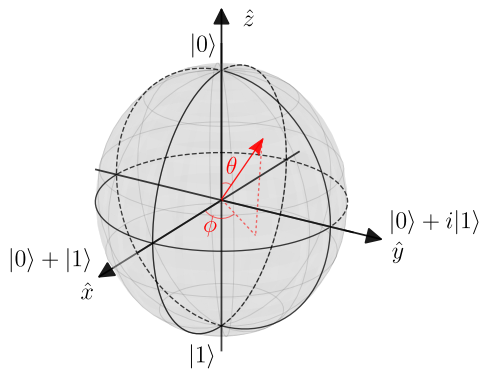
\includegraphics[width=0.35\textwidth]{figures/png/BlochSphere.png}
\caption{Example of qubit state representation on the Bloch sphere\\
Source: Metrology of Quantum Control and Measurement in Superconducting Qubits \cite{Chen2018}}
\label{fig:BlochSphere}
\end{figure}

The qubit states $\ket{0}$ and $\ket{1}$ can also be associated with energy eigenstates of a physical system, where $\ket{0}$ represents the ground state with energy $E_0$ and $\ket{1}$ represents the excited state with energy $E_1$, assuming $E_0 < E_1$. 
In this energy eigenbasis, the Hamiltonian of the qubit is given by
\begin{equation}\label{eq:qubithamiltonian}
    \hat{H}_q = E_0 \ket{0} \bra{0} + E_1 \ket{1} \bra{1} = 
    \begin{pmatrix}
        E_0 & 0 \\
        0 & E_1
    \end{pmatrix}.
\end{equation}

Since only energy differences are physically relevant, it is possible to redefine the zero-point energy by subtracting the constant term $E_0 (\ket{0} \bra{0} + \ket{1} \bra{1})$, leading to the simplified Hamiltonian
\begin{equation}\label{eq:qubithamiltonian}
    \hat{H}_q = (E_1 - E_0) \ket{1} \bra{1} = \hbar \omega_q \ket{1} \bra{1} = \hbar \omega_q \hat{\sigma}^{+} \hat{\sigma}^{-} = 
    \begin{pmatrix}
        0 & 0 \\
        0 & \hbar \omega_q
    \end{pmatrix},
\end{equation}

where $\omega_q = (E_1 - E_0)/\hbar$ is the qubit transition frequency, and we have used the relation $\hat{\sigma}^{+} \hat{\sigma}^{-} = \ket{1} \bra{1}$.
For convenience, the Hamiltonian can also be rewritten in terms of the Pauli $z$-matrix, $\hat{\sigma}_z$, by adding a term proportional to the identity:
\begin{equation}
    \hat{H}_q = \hbar \omega_q \ket{1} \bra{1} - \frac{\hbar \omega_q}{2}\mathbb{I} = 
    \begin{pmatrix}
        -\frac{\hbar \omega_q}{2} & 0 \\
        0 & \frac{\hbar \omega_q}{2}
    \end{pmatrix} = -\frac{\hbar \omega_q}{2} \hat{\sigma}_z.
\end{equation}

\paragraph{}
Qubits can be implemented through various physical mechanisms; however, their practical realization remains a significant challenge due to their susceptibility to environmental interactions, which lead to decoherence and reduce their coherence time. 
Despite the diversity of possible physical implementations, any functional quantum computing system must satisfy a set of fundamental criteria. 
These requirements, known as the DiVincenzo criteria, establish the essential conditions for the construction and operation of a viable quantum computer \cite{DiVincenzo_2000}, \cite{manenti_quantum_2023}:
\begin{enumerate}
    \item The physical system used as quantum computer must comprise a set of qubits, meaning that the quantum system must be well-characterized, and scalable such that quantum
    computing can be realized.
    \item It must be possible to initialize the qubits in a reliable state, such as the ground state.
    \item The coherence time of the qubits must be longer than the typical gate time, ideally should be possible to perform $>10^4$ operations, that is the number which allows for realizing effective error corrections.
    \item It must be possible to implement a universal set of quantum gates.
    \item It must be possible to measure the qubits in the computational basis.
\end{enumerate}

In the present work, I will focus on superconducting qubits, which constitute the hardware I have worked on and where the experiments were conducted. 
However, several of the experiments described later can also be implemented using different physical systems.

\section{Transmon qubits}
In this section, I provide a review of the structure and operation of superconducting transmon qubits. 
The content of this section is based on the \textit{Quantum Information Science} manual \cite{manenti_quantum_2023}, \textit{The Metrology of Quantum Control and Measurement in Superconducting Qubits} \cite{Chen2018}, the notes from quantum computing lectures held by Professor Olivares \cite{Olivares2021}, and the original transmon paper \cite{TransmonPaper}.

\subsection{Josephson Junctions}
The Josephson junction (JJ) is formed by a thin oxide layer positioned between the two superconductors which acts as an insulating barriers. 
An example of Josephson junction is show in figure \ref{fig:JJ}, a side view in image \ref{fig:JJ_side} and a top view in image \ref{fig:JJ_top}.
\begin{figure}[ht!]
    \centering
    \begin{subfigure}{0.45\textwidth}
        \centering
        
\includegraphics[width=0.90\textwidth]{figures/png/JJ_side.png}
        \subcaption{}
        \label{fig:JJ_side}
    \end{subfigure}
    \hfill
    \begin{subfigure}{0.45\textwidth}
        \centering
        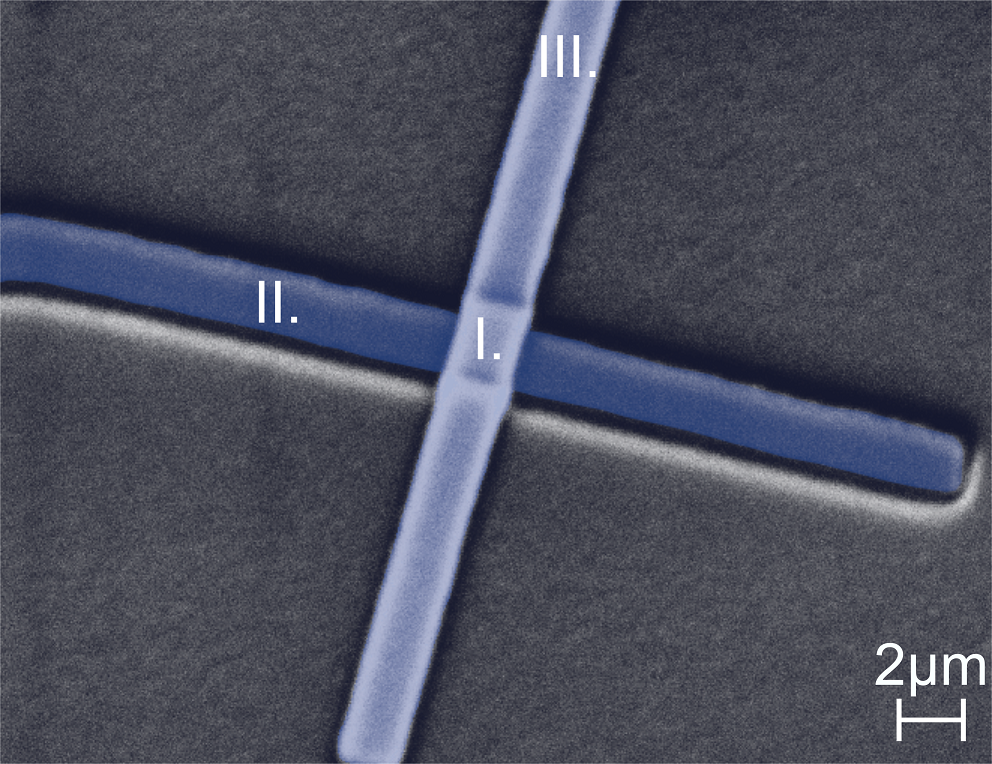
\includegraphics[width=0.70\textwidth]{figures/png/JJ_top.png}
        \subcaption{}
        \label{fig:JJ_top}
    \end{subfigure}
    \caption{Figure \ref{fig:JJ_side}: Side viwe of a Josephson junction, the two superconducting pads are coloured in red and blue and indicating by the letter S. In grey, indicated by letter I is represented the insulating barrier of oxide. 
    The superconductors and the oxide are layered over a substrate.\\
    Figure \ref{fig:JJ_top}: Electron microscope image of a $2 \mu\text{m} \cross 2 \mu\text{m}$ cross-type junction: I. Josephson junction. II. Base electrode. III. Contact to the top electrode.\\
    Source:\url{https://www.ims.kit.edu/english/2551.php}}
    \label{fig:JJ}
\end{figure}

Superconductivity is a phenomenon observed in certain materials where, when cooled well below a critical temperature $T_c$, which depends on the material, their electrical resistance drops to zero, allowing them to behave as perfect conductors.
According to the BCS (Bardeen-Cooper-Schrieffer) theory, superconductivity arises, from the formation of Cooper pairs, which are bound states of electrons with opposite momenta and spins.
These pairs collectively forms a macroscopic quantum states described by a single waveform $\psi(\mathbf{r})$ which can be expressed as 
\begin{equation}\label{eq:BCSequation}
    \psi(\mathbf{r}) = \sqrt{\rho(\mathbf{r})}e^{i\theta(\mathbf{r})}
\end{equation}
where $\rho(\mathbf{r})$ is the density of Cooper pairs in the metal, which is typically uniform in the bulk of the superconductor, and $\theta(\mathbf{r})$ is the macroscopic phase of the superconducting wavfunction.

For this reason the wavefunctions on the two sides of the JJ can be denoted as
\begin{equation}\label{eq:JosephsonWavefunctions}
    \psi_1(\mathbf{r}, t) = \sqrt{\rho_1(\mathbf{r}, t)} e^{i\theta_1(\mathbf{r},t)}, \psi_2(\mathbf{r}, t) = \sqrt{\rho_2(\mathbf{r}, t)} e^{i\theta_2(\mathbf{r},t)}
\end{equation}

The dynamics of the system can be described by the two equations\begin{equation}\label{eq:schr1}
    i\hbar \frac{d\psi_1}{dt} = E_1 \psi_1 + K \psi_2,
\end{equation}
\begin{equation}\label{eq:schr2}
    i\hbar \frac{d\psi_2}{dt} = E_2 \psi_2 + K \psi_1.
\end{equation}
By substituting the expression of $\psi_i$ into the Schr\"odinger equation \ref{eq:schr1}, \ref{eq:schr2} we obtain
\begin{equation}\label{eq:schr-sub1}
    \frac{d\rho_1}{dt} = \frac{2K}{\hbar} \sqrt{\rho_1 \rho_2} \sin(\theta_2 - \theta_1),
\end{equation}
\begin{equation}\label{eq:schr-sub2}
    \frac{d\rho_2}{dt} = -\frac{2K}{\hbar} \sqrt{\rho_1 \rho_2} \sin(\theta_2 - \theta_1).
\end{equation}

Since the derivative of the charge density is the current, from equations \ref{eq:schr-sub1} and \ref{eq:schr-sub2} we obtain the first Josephson equation
\begin{equation}\label{eq:Josephson1}
    I=I_c\sin{\phi}
\end{equation} 
where $I_c = \frac{2K}{\hbar}\sqrt{\rho_1\rho_2}$ is the critical current and $\phi$ is the superconducting phase difference $\theta_2 - \theta_1$.

Instead, from the real part of the Schr\"odinger equation \ref{eq:schr1}, \ref{eq:schr2} and a few calculations, we obtain the second Josephson equation
\begin{equation}\label{eq:Josephson2}
    \frac{d\phi}{dt} = \frac{2e}{\hbar} V(t).
\end{equation}
which can be rewritten as \begin{equation}
    \frac{d\phi}{dt} = \frac{2\pi}{\Phi_0} V(t).
\end{equation}
where $\Phi_0 = \frac{h}{2e}$ is the superconducting flux quantum, with $h$ is the Planck's constant and $2e$ is the charge of a Cooper pair.

The time derivative of the first Josephson equation \ref{eq:Josephson1} yields:
\begin{equation}\label{eq:current_derivative}
    \dot{I_J}=I_C\cos{\phi}\frac{\partial \phi}{\partial t},
\end{equation}
equation \ref{eq:current_derivative} suggests a nonlinear relation between the current the voltage. 
Using the Josephson voltage-phase relation and the fact that $\dot{I}=\frac{V}{L}$ it is possible to define an effective nonlinear inductance for the Josephson junction:
\begin{equation}\label{eq:LJ}
    L_J = \frac{1}{\cos{\phi}}\frac{\Phi_0}{2\pi I_c}.
\end{equation} 

In addition to ths inductive behaviour the Josephson junction also exibits capacitive properties due to its inherent capacitance $C_J$ with a corresponing energy of 
\begin{equation}\label{eq:capacitive_energy}
    E_{C_J} = \frac{Q^2}{2C_J}
\end{equation}.

Fom equation \ref{eq:LJ} it is possible to compute the energy stored in the nonlinear inductance as
\begin{align}\label{eq:inductive_energy}
    E_{L_J} &= \int_{0}^{t}\text{d}\tau I_J(\tau)V(\tau) = \int_{0}^{t}\text{d}\tau I_c\sin{\phi(\tau)}\frac{\partial\phi(\tau)}{\partial\tau}\frac{\Phi_0}{2\pi}\\
    &= \frac{\Phi_0 I_c}{2\pi}(1-\cos{\phi}) = E_J(1-\cos{\phi})
\end{align}
where $E_J$ represents the energy due to the behaviour of the junction as nonlinear inductor .

\subsection{CPB qubit}

A first example of superconducting qubit is the Cooper Pair Box (CPB), which consists of a small superconducting island connected to a reservoir of superconducting electrons through a Josephson junction \cite{Vion2002}, with an external gate voltage controlling the charge state.
The circuit corresponding to CPB is similar to the circuit of a parallel resonator where the linear inductance is subsituted by a Josephson junction which simply acts as a nonlinear inductance.

Combining the energy associated to the capacitance $C$ and the energy of the Josephson junction \ref{eq:inductive_energy} it is possible to write the classical Hamiltonian of the circuit
\begin{equation}\label{eq:CPB_hamiltonian}
    H_J = 4E_C n^2 - E_J\cos{\phi}
\end{equation}
where the constant term was ignored as it acts simply as a constant offset without influencing the dynamics of the system and where $E_C$ is the charging energy defined as \begin{equation}\label{eq:charging_energy}
    E_C = \frac{e^2}{2C}.
\end{equation}

\begin{figure}[ht!]
    \centering
    \begin{subfigure}{0.45\textwidth}
        \centering
        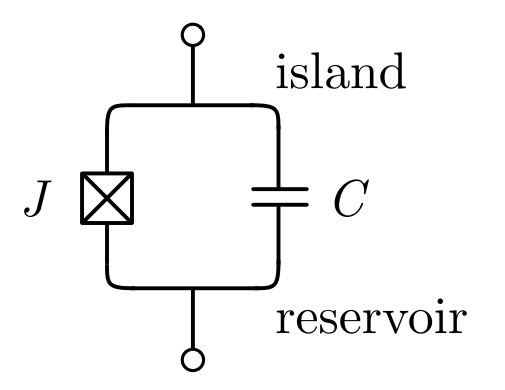
\includegraphics[width=0.60\textwidth]{figures/png/CPB.png}
        \subcaption{}
        \label{fig:CPB}
    \end{subfigure}
    \hfill
    \begin{subfigure}{0.45\textwidth}
        \centering
        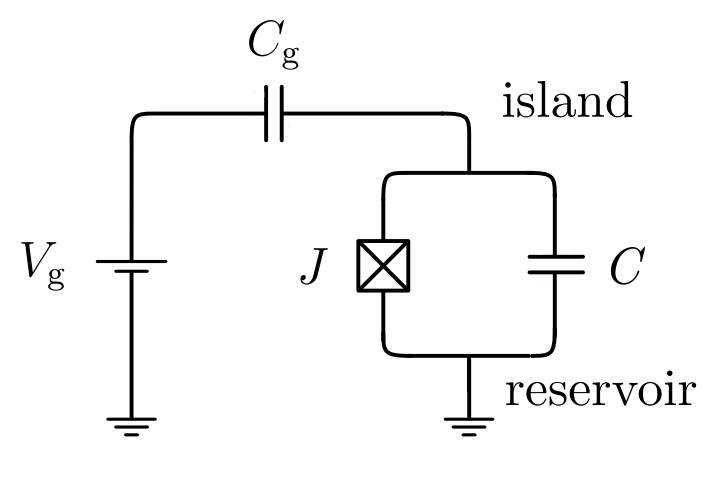
\includegraphics[width=0.70\textwidth]{figures/png/CPB_circuit.png}
        \subcaption{}
        \label{fig:CPB_circuit}
    \end{subfigure}
    \caption{Figure \ref{fig:CPB}: corresponding circuit of a CPB which consists of Josephson junction shunted by a capacitor. Surce: \cite{manenti_quantum_2023}. Figure \ref{fig:CPB_circuit}: electrical circuit of a CPB capacitively coupled to a DC voltage source through a capacitor $C_g$. Source: \cite{manenti_quantum_2023}.}
    \label{fig:CPB_general}
\end{figure}

To control the number of Cooper pairs on the island, it is possible to connecnt a DC voltage source $V_g$ to the system through a gate capacitor $C_g$, as shown in Figure \ref{fig:CPB_circuit}.
When $V_g = 0$, both the gate and qubit capacitors remain uncharged. 
As $V_g$ increases, a charge $Q_g = C_g V_g$ accumulates on the gate capacitor, inducing an equal and opposite charge on the island to maintain charge neutrality. 
When $Q_g \approx 2e$, a Cooper pair tunnels from the reservoir to the island, discharging the qubit capacitor. \\

The presence of the external voltage source introduces an additional control parameter for the number of Cooper pairs on the island, modifying the system's Hamiltonian. 
The resulting Hamiltonian of the Cooper Pair Box (CPB) takes the form

\begin{equation}\label{eq:CPB_complete}
    \hat{H} = 4E_C(\hat{n} - n_g)^2 - E_J \cos{\hat{\phi}}
\end{equation}

where $n_g = \frac{C_g V_g}{2e}$ represents the normalized gate charge.

A key feature of the system is the presence of a Josephson junction in place of a linear inductance. 
Unlike a standard LC circuit—corresponding to a quantum harmonic oscillator—this results in a non-equidistant energy level spectrum. 
In particular, the energy levels are anharmonic, allowing the first two levels to be spectrally isolated from the higher ones. 
This anharmonicity enables the use of the subspace spanned by the ground state $\ket{0}$ and the first excited state $\ket{1}$ aas a qubit.

The qubit frequency is defined as the frequency associated with the energy difference between these two states: $f_{01}(n_g) = f_Q = \frac{(E_1 - E_0)}{h}$.
This frequency can be tuned by varying the externally applied DC voltage, which modifies the system’s parameters and, consequently, its energy level spacing.\\

%%%NOTA PER ME: INSERIRE IL PLOT DEI LIVELLI ENERGETICI DEL CPB


\subsection{Transmon qubit}
One of the main drawbacks of the Cooper Pair Box (CPB) qubit, which ultimately led to its replacement by other qubit architectures, is its limited coherence time. 
The transmon qubit was introduced specifically to address this issue, with the goal of improving the dephasing time of the CPB. The key idea behind the transmon is to reduce the sensitivity of the energy levels to fluctuations in the gate charge—effectively flattening the energy bands—by increasing the ratio between the Josephson energy $E_J/E_C \geqq 1$,
this architecture was first proposed in \cite{TransmonPaper}, the first and more straightforward method to increase this ratio is to enlarge the capacitance of the qubit, which reduces the charging energy $E_C$.

Since the CPB and the transmon qubit have the same electrical circuit they are also described by the same Hamiltonian \ref{eq:CPB_hamiltonian}. 
The difference is that in this case the transmon satisfies the condition $E_J/E_C \geqq 1$ it is possible to expand the cosine term in \ref{eq:CPB_hamiltonian} with a Taylor series and neglect the higher order terms:
\begin{equation}\label{eq:approx_transmon}
    \hat{H}\approx 4E_C\hat{n}^2 + \frac{1}{2}E_J\hat{\phi}^2 - \frac{E_J}{4!}\hat{\phi}^4
\end{equation}
where the last term, proportional to $\hat{phi}^4$, makes the potential of the transmon slightly anharmonic.

As happens in the standard harmonic oscillator case, the operators $\hat{phi}$ and $\hat{n}$ satisfy the cnaonical commutation relation $[\hat{\phi},\hat{n}]=i\mathbb{I}$, it is possible to introduce the raising and lowering operators $\hat{b},\hat{b}^\dagger$ as
\begin{equation}\label{eq:raising_lowering_operators}
    \hat{\phi} = \sqrt{\xi}(\hat{b}+\hat{b}^\dagger), \quad\quad \hat{n} = -\frac{i}{2\sqrt{xi}}(\hat{b}-\hat{b}^\dagger),
\end{equation}
where $\xi =  \sqrt{2E_C/E_J}$.

Substituting equations \ref{eq:raising_lowering_operators} in the Hamiltonian, equation \ref{eq:approx_transmon} becomes
\begin{equation}\label{eq:transmon_hamiltonian}
    \hat{H} = \sqrt{8E_JE_C}\hat{b}^\dagger\hat{b} - \frac{E_C}{12}(\hat{b}+\hat{b}^\dagger)^4.
\end{equation}

Given equation \ref{eq:transmon_hamiltonian} it is possible to solve the eigenvalue proble $\hat{H}\ket{k}=E_k\ket{k}$ and calculate the energy levels $E_k$.
The first term of Hamiltonian \ref{eq:transmon_hamiltonian} is the harmonic oscillator contribution with eigenstates $\ket{k}$ and eigenvalues $\sqrt{8E_JE_C}k$. 
Since $E_C \ll E_J$, the second term $ \hat{V} = -\frac{E_C}{12}(\hat{b} + \hat{b}^\dagger)^4$ represents a small perturbative contribution to the Hamiltonian and can be treated using perturbation theory. 
The first-order correction to the energy levels is given by the diagonal matrix elements of the perturbation operator: $\Delta E_k^{(1)} = \langle k | \hat{V} | k \rangle$.
It is possible to verify that $\bra{k} \hat{V} \ket{k} = -\frac{E_C}{12} (6k^2 + 6k + 3)$. 
Thus the eigenenergies of the transmon Hamiltonian are 
\begin{equation}
    E_k \approx \sqrt{8E_JE_C}k - \frac{E_C}{2}(k^2 + k).
\end{equation}

As mentioned before, the qubit frequency is defined as $f_Q = f_{01} = (E_1 - E_0)/h$ which yields
\begin{equation}
    f_01 \approx (\sqrt{8E_JE_C} - E_C)/h
\end{equation}

As explained at the beginning of this section, a large $E_J/E_C$ ratio makes the transmon qubit significantly less sensitive to charge noise. 
However, this improvement comes at the expense of reduced anharmonicity in the energy level spectrum. 
The anharmonicity $\eta$ is defined as the difference between the second and first transition energies, relative to the first transition energy:
\begin{equation}
    \eta = \frac{(E_2 - E_1) - (E_1 - E_0)}{\hbar} = \omega_{12} - \omega_{01}.
\end{equation}
For a transmon, the anharmonicity $\eta$ is negative, reflecting the fact that the level spacing decreases with increasing energy. 
Ideally, the absolute value  $|\eta|$ should be sufficiently large to allow external microwave drives to selectively address the $\ket{0}\leftrightarrow\ket{1}$ transition without inadvertently exciting higher-energy states.


\subsection{Flux-tunable transmon}
To implement certain two-qubit gate schemes, such as swap interactions, it is essential to tune the qubit frequency. 
A common approach to achieving this is by adding an extra junction to the transmon, the most common configuration is the SQUID (Superconducting QUantum Interference Device).
In the SQUID configuration two Josephson junctions are connected in parallel on a superconducting loop, as shown in Figure \ref{fig:FrequencyTunableTransmon}.

Starting from the Hamiltonian of the single Josephson junction it is possible to write the Hamiltonian of a SQUID:
\begin{equation}\label{eq:SQUID_Hamiltonian}
    \hat{H} = 4E_C\hat{n}^2 - E_{J1}\cos{\hat{\phi_1}} - E_{J2}\cos{\hat{\phi_2}}
\end{equation}
where $E_{J1}$ and $E_{J2}$ are the Josephson energies of the two junctions, and the operators $\hat{\phi_1}$ and $\hat{\phi_2}$ are the phase differences across the junctions.

Because od the quantization of the magnetic flux through the SQUID, the quantities $\hat{\phi_1}$ and $\hat{\phi_2}$ are not independet. 
In particular, as show in \cite{manenti_quantum_2023}, the difference between $\hat{\phi_1}$ and $\hat{\phi_2}$ follows the following relation:
\begin{equation}\label{eq:phases_relation}
    \hat{\phi_1} - \hat{\phi_2} = \frac{2\pi}{\Phi_0}\Phi_{\text{ext}}\mathbb{I}(\text{mod}2\pi)
\end{equation}
where $\Phi_{\text{ext}}$ is the flux of external magnetic field defined as the integral of the magnetic field over the SQUID area.

Equation \ref{eq:phases_relation} can be simplified and rewritten as 
\begin{equation}\label{eq:tunable_transmon_hamiltonian}
    \hat{H} = 4E_C\hat{n}^2 - E_J(\Phi_{\text{ext}})\cos{\hat{\varphi}}
\end{equation}
where $\hat{\varphi} = \frac{\hat{\phi_1}+\hat{\phi_2}}{2}$, and the Josephson energy is flux-dependent: 
\begin{equation}\label{eq:EJ_tunable}
    E_J(\Phi_{\text{ext}}) = (E_{J1} + E_{J2}) \left| \cos \left( \pi \frac{\Phi_{\text{ext}}}{\Phi_0} \right) \right| \sqrt{1 + d^2 \tan^2 \left( \pi \frac{\Phi_{\text{ext}}}{\Phi_0} \right) },
\end{equation}
where $d = \frac{E_{J1}-E_{J2}}{E_{J1}+E_{J2}}$ is the relative junction asymmetry.

Then, it's easy to see that the frequency $f_Q$ of a two-junction transmon dependends on the magnetic flux $\Phi_Q(t)$ through the SQUID loop, for symmetric junctions is given by
\begin{equation}\label{eq:freqdepndenceonflux}
    f_Q(\Phi_Q) \approx \frac{1}{h} \left( \sqrt{8E_J E_C \cos\left(\pi \frac{\Phi_Q}{\Phi_0} \right)} - E_C \right).    
\end{equation}

\begin{figure}[ht!]
    \centering
    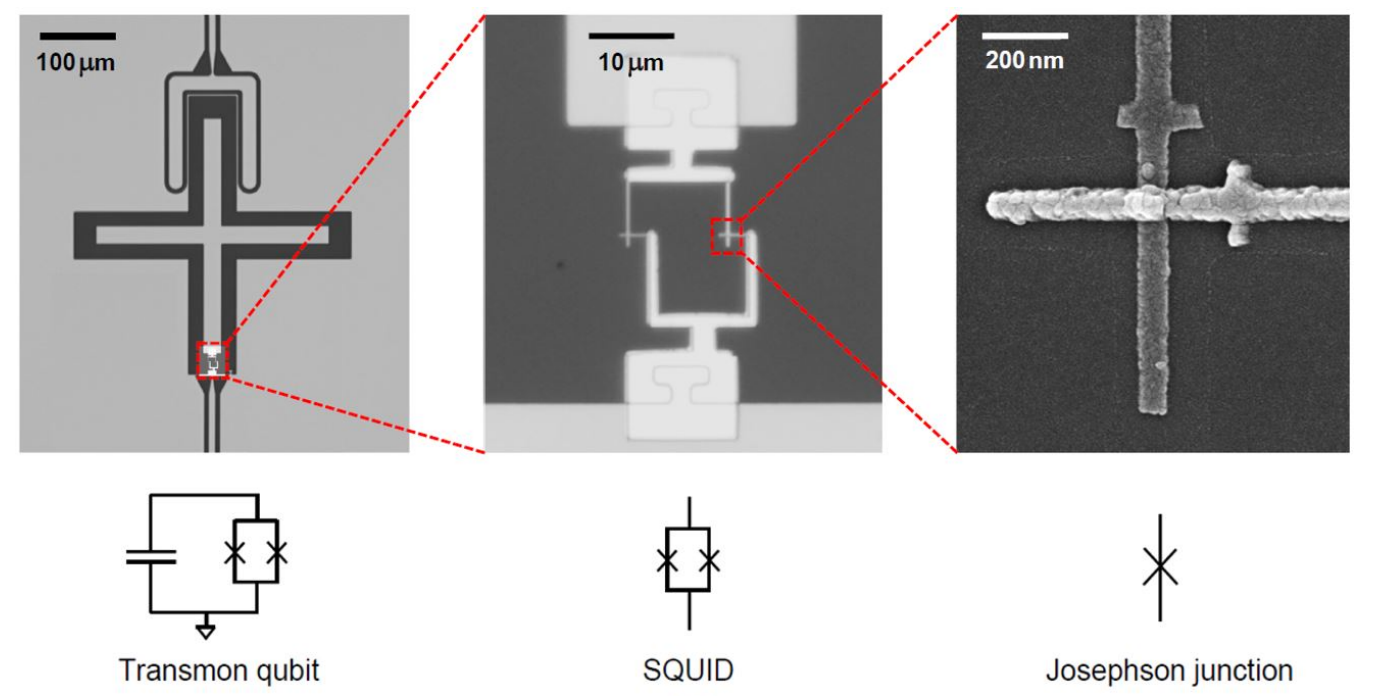
\includegraphics[width=0.50\textwidth]{figures/png/FrequencyTunableTransmon.png}
    \caption{Images of a flux tunable transmon qubit. From left to right: the flux tunable transmon qubit, consisting of a large cross-shaped capacitance in parallel with a SQUID to ground, and its corresponding circuit. A zoom in of the SQUID (center), a single Josephson junction (right). Source: \cite{Roth_2023}}
    \label{fig:FrequencyTunableTransmon}
\end{figure}


\section{Qubit readout}\label{sec:cQED}
Up to this point, I have discussed the physical structure of a transmon qubit. 
However, in order to perform quantum computing, it is essential to be able to control and measure its quantum state.
One approach to achieve this is to capacitively couple the qubit to both a drive line and a readout line. 
The drive line is used to manipulate the state of the qubit, while the readout line is employed to measure it.
An example of such a system is shown in Figure \ref{fig:Transmon_model}, along with the corresponding circuit diagram.

\begin{figure}[h!]
    \centering
    \begin{subfigure}{0.47\textwidth}
        \centering
        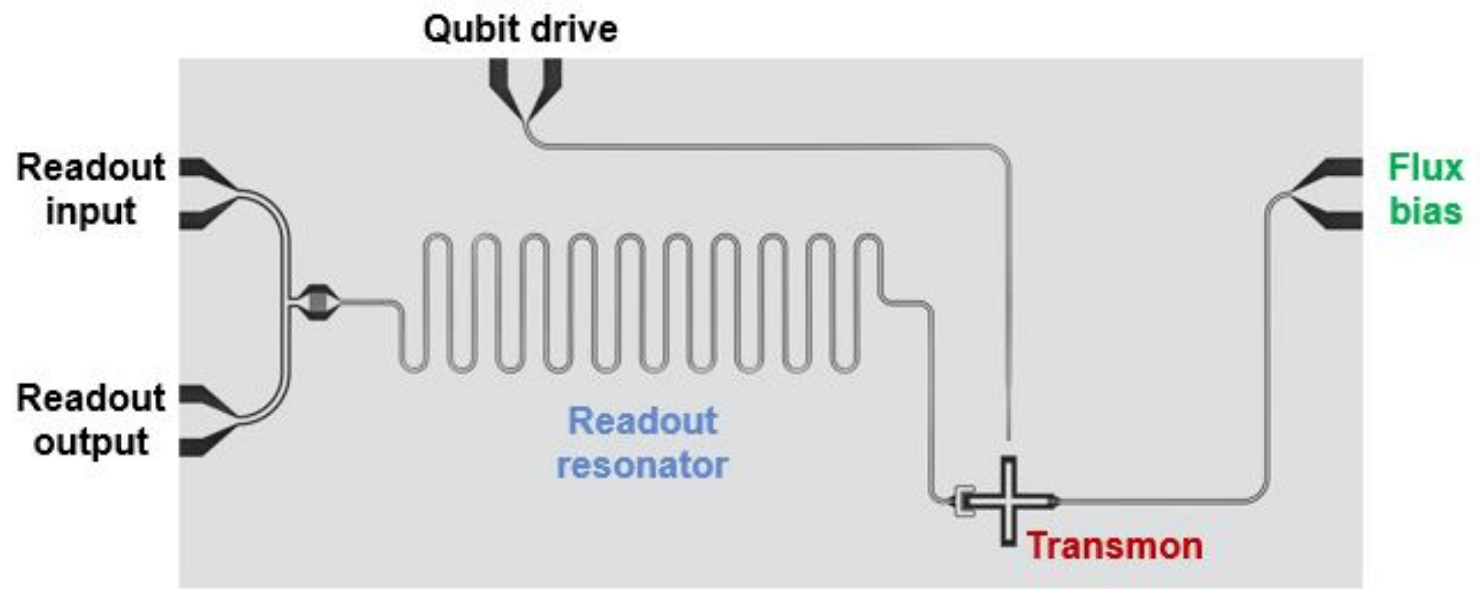
\includegraphics[width=\textwidth]{figures/png/TransmonBoard.png}
        \subcaption{}
        \label{fig:TransmonBoard}
    \end{subfigure}
    \hfill
    \begin{subfigure}{0.47\textwidth}
        \centering
        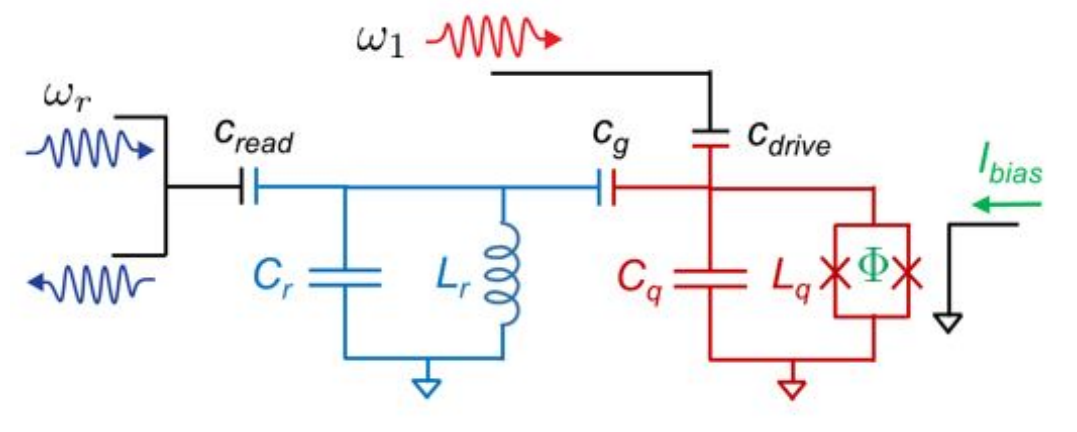
\includegraphics[width=\textwidth]{figures/png/TransmonCircuit.png}
        \subcaption{}
        \label{fig:TransmonCircuit}
    \end{subfigure}
    \caption{Figure \ref{fig:TransmonBoard} shows an example of a single transmon device. Figure \ref{fig:TransmonCircuit} shows the equivalent lumped element circuit model of the device in \ref{fig:TransmonBoard}, in blue is represented the resonator circuit while in red the transmon qubit circuit. Source: \cite{Roth_2023}}
    \label{fig:Transmon_model}
\end{figure}

As mentioned in the introduction of this section, in circuit quantum electrodynamiccs (cQED), the qubit state is measured via a dispersive interaction between a qubit and a far-detuned microwave resonator.\\

In Figure \ref{fig:TransmonCircuit}, in blue is represented the resonator circuit capacitively coupled to the (red) qubit that is used for the readout of the qubit state. 
The resonator circuit is characterized by a an inductance $L_r$ and a capacitance $C_r$, then the characteristic frequency is $\omega_r =  1/\sqrt{L_r C_r}$. 

The classical Hamiltonian of the resonator can be written as 
\begin{equation}\label{eq:classical_hamiltonian_resonator}
    H_r = \frac{Q^2}{2C_r} +  \frac{1}{2}C\omega_r^2\Phi^2,
\end{equation}

where $\Phi$ is the generalized flux, defined as the time integral of the voltage across the capacitor:
\begin{equation}\label{eq:generalized_flux}
    \Phi(t) = \int_{-\infty}^{t} V(t')dt' .
\end{equation}.

The quantization of the Hamiltonian involves replacing the classical conjugate variables with their corresponding hermitian operators $\hat{\Phi}$ and $\hat{Q}$ with $[\hat{\Phi},\hat{Q}]=i\hbar\mathbb{I}$ which leads to
\begin{equation}
    \hat{H}_r = \frac{\hat{Q}^2}{2C_r} +  \frac{1}{2}C\omega_r^2\hat{\Phi}^2.
\end{equation}
To find the eigenvalues ans eigenvectors of $\hat{H}_r$ it is often convenient to introduce the raising and lowering operators, $\hat{a}$ and $\hat{a}^\dagger$ which satisfy $[\hat{a},\hat{a}^\dagger]=\mathbb{I}$.
These two non-hermitian operators are defined as 
\begin{equation}\label{eq:Phi_operator}
    \hat{\Phi} =  \Phi_{\text{zpf}}(\hat{a} + \hat{a}^\dagger),
\end{equation}
\begin{equation}\label{eq:Q_operator}
    \hat{Q} = -iQ_{\text{zpf}}(\hat{a} - \hat{a}^\dagger)
\end{equation}
where $\Phi_{\text{zpf}} = \sqrt{\frac{\hbar}{2C_r\omega_r}}$ and $Q_{\text{zpf}} = \sqrt{\frac{C_r\hbar \omega_r}{2}}$ are the zero-point fluctuations.

Then it is possible to write the Hamiltonian of a microwave resonator in a quantum regime:

\begin{equation}\label{eq:quant_resonator_hamiltonian}
    \hat{H}_r = \hbar\omega_r\left(\hat{a}^\dagger\hat{a} + \frac{1}{2}\right),
\end{equation}

The system of the capacitively coupled transmon and resonator is built in such a way that there is a maximum coupling between the qubit and the resonator.
The Hamiltonian of the system reads
\begin{align}
    \hat{H} &= \hbar \omega_r \hat{a}^\dagger \hat{a} + 4E_C (\hat{n} + \frac{C_{\text{read}}\hat{V}}{2e})^2- E_J \cos\hat{\phi}\\ 
    &= \hbar \omega_r \hat{a}^\dagger \hat{a} + 4E_C \hat{n}^2 - E_J \cos\hat{\phi} + \frac{4E_C}{e} \hat{n}_C \hat{V}
\end{align}
where $\hat{V} = \hat{Q}/C_r$ is the voltage across the resonator capacitor. Using equations \ref{eq:raising_lowering_operators} and \ref{eq:quant_resonator_hamiltonian} the Hamiltonian becomes
\begin{equation}
    \hat{H} = \hbar \omega_r \hat{a}^\dagger \hat{a}  + \sqrt{8 E_J E_C} \, \hat{b}^\dagger \hat{b} - \frac{E_C}{12} (\hat{b} + \hat{b}^\dagger)^4 + \hbar g (\hat{b}^\dagger - \hat{b})(\hat{a} - \hat{a}^\dagger)
\end{equation}
where was introduced the parameter $g$, known as coupling strength, that quantities the strength of the coupling between the qubit and the resonator.:

\begin{equation}
    g = \frac{2 E_C}{\hbar e} \frac{C_{\text{read}}}{C_r} Q_{\text{zpf}} \sqrt{\xi} = \frac{E_C}{\hbar e} \left( \frac{E_J}{2 E_C} \right)^{1/4} \frac{C_{\text{read}}}{C_r} \sqrt{2 \hbar \omega_r C_r}.
\end{equation} 
The coupling strength can be adjust by varying the capacitance coupling the qubit and the resonator.

When $g\ll\omega_r$ and $g\ll\omega_q$ it is possible to use the rotating wave approximation (RWA) and write the Hamiltonian in the form
\begin{equation}
    \hat{H} = \hbar \omega_r \hat{a}^\dagger \hat{a} + \sqrt{8E_J E_C} \hat{b}^\dagger \hat{b} - \frac{E_C}{12} (\hat{b} + \hat{b}^\dagger)^4 + \hbar g (\hat{b}^\dagger \hat{a} + \hat{b} \hat{a}^\dagger).
\end{equation}

Focusing on the first two levels of the transmon we obtain the Jaynes-Cummings Hamiltonian that reads
\begin{equation}\label{eq:Jaynes-Cummings}
    \hat{H} = \hbar \omega_r \hat{a}^\dagger \hat{a} - \frac{\hbar \omega_{01}}{2} \hat{\sigma}_z + \hbar g (\hat{\sigma}_+ \hat{a} + \hat{\sigma}_- \hat{a}^\dagger),
\end{equation}
that describes the interaction between an atom, in this case an artificial atom, with an electromagnetic field in the approximation of the two-level system.

When the coupling strength $g$ is much smaller than the detuning between the qubit and the resonator $\Delta = \omega_q -\omega_r $ the system operates in the dispersive regime.

The Jaynes-Cummings Hamiltonian in the dispersive regime, which is the condition in which we operate to perform the qubit readout, can be approximated as 
\begin{equation}\label{eq:dispersiveshift_hamiltonian}
    \hat{H}_{\text{disp}} = \hbar (\omega_r - \chi \hat{\sigma}_z) \hat{a}^\dagger \hat{a} - \frac{\hbar}{2} (\omega_{01} + \chi) \hat{\sigma}_z
\end{equation}
where $\chi$ is the dispersive shift defined as \begin{equation}\label{eq:dispersiveshift}
    \chi = \frac{g^2}{\Delta}.
\end{equation}

Equation \ref{eq:dispersiveshift_hamiltonian} shows that there is a shift in the resonator frequency from $\omega_r$ to $\omega_r - \chi$ if the qubit is in the ground state and a shift from $\omega_r$ to $\omega_r + \chi$ if the qubit is in the excited state.

The dispersive shift equation \ref{eq:dispersiveshift} was derives assuming that the qubit can be approximated as a two level system.
Considering also the higher energy levels of the qubit a more accurate expression of the dispersive shift is given by 
\begin{equation}
    \chi = \frac{g^2}{\Delta(1+\Delta/\eta)}
\end{equation} 
where $\eta$ is the qubit anharmonicity.

\section{Qubit control}
Another necessary element for performing quantum computation is the implementation, starting with single-qubit gates. 
A qubit can be driven into any arbitrary superposition state by applying an electrical pulse with a carefully controlled amplitude, duration, and phase.
This pulse is generated by an AC voltage source located outside the dilution refrigerator that hosts the qubit.
The driving pulse is brought to the qubit by an on-chip waveguide which is capacitively coupled to the qubit as shown in Figure \ref{fig:TransmonCircuit}, where the coupling capacitance is indicated with $c$.
This signal path is commonly referred to as a control line or an XY line. The pulse that arrives at the device has the analytical form
\begin{equation}\label{eq:drive_pulse}
    V_d(t) = A\varepsilon(t)\sin{\omega_d t + \alpha}
\end{equation}
where $A$ is the pulse amplitude in volts, $\omega_d$ is the drive frequency in rad/s, $\alpha$ is the fase of the pulse and $\varepsilon(t)$ is the modulation of the pulse; the maximum of $\varepsilon(t)$ is fixed at one.
As a first approximation, the envelope of the drive pulse is often chosen to have a Gaussian shape, which is preferred over a square pulse due to its smaller frequency bandwidth, minimizing the excitation of higher energy levels.
However, the study of pulse shapes that minimize leakage to states outside the computational basis remains an active area of research \cite{chiaro2025activeleakagecancellationsingle}.

In a similar way to what was previously done to study the capacitive coupling between the qubit and the resonator, it is possible to derive th hamiltonian of the transmon capacitively coupled to the control line starting from the circuit shown in Figure \ref{fig:TransmonCircuit}
\begin{equation}
    \hat{H} = 4E_C(\hat{n} + \frac{C_d V_d(t)}{2e})^2 - E_J \cos{\hat{\phi}}
\end{equation}, 
where $E_C = e^2/2C_\Sigma$ and $C_\Sigma =  C_d + C_q$. By expanding the parenthesis and dropping a constant term the Hamiltonian can be re-written as
\begin{equation}\label{eq:tmp}
    \hat{H} =  4E_C\hat{n}^2 -E_J\cos{\hat{\phi}} + 2e\frac{C_d}{C_\Sigma}V_d(t)\hat{n}.
\end{equation}
Since $\hat{n} = -i(\hat{b}-\hat{b}^\dagger)/2\sqrt{\xi}$ (from equation \ref{eq:raising_lowering_operators}), the last term of the Hamiltonian can be rewritten:
\begin{align}\label{eq:misto}
    \hat{H}_d &= -2e\frac{C_d}{C_\Sigma}V_d(t)\hat{n}\\
    &=-i\frac{e}{\sqrt{\xi}}\frac{C_d}{C_{\Sigma}}V_d(t)(\hat{b}-\hat{b}^\dagger)\\
    &=-i\frac{e}{\sqrt{\xi}}\frac{C_d}{C_{\Sigma}}V_d(t)(\ket{0}\bra{1}-\ket{1}\bra{0})\\
    &=\frac{e}{\sqrt{\xi}}\frac{C_d}{C_{\Sigma}}V_d(t)\hat{\sigma_y}
\end{align}

Regarding the first part of equation \ref{eq:tmp}, by focusing on the firs two levels of the transmon the qubit Hamiltonian can be rewritten as $\hat{H}_q = -\frac{1}{2}\hbar\omega_q\hat{\sigma}_z$.
Then, by substituting the qubit and drive Hamiltonians (equation \ref{eq:misto}) and the analytical form of $V_d(t)$ in equation \ref{eq:tmp} we obtain
\begin{align}
    \hat{H} &= \hat{H}_q + \hat{H}_d = -\frac{\hbar \omega_q}{2} \hat{\sigma}_z + \frac{e}{\sqrt{\xi}} \frac{C_g}{C_{\Sigma}} A \epsilon(t) \sin(\omega_d t + \alpha) \hat{\sigma}_y\\
    &= = -\frac{\hbar \omega_q}{2} \hat{\sigma}_z + \hbar \Omega \epsilon(t) \sin(\omega_d t + \alpha) \hat{\sigma}_y,
\end{align} 
where $\Omega$ is the Rabi frequency, 
\begin{equation}
    \Omega = \frac{e}{\hbar\sqrt{\xi}}\frac{C_d}{C_\Sigma}A.
\end{equation}
The Rabi frequency quantifies the coupling between the control line and the qubit.

To study the dynamics of the system it is convenient to use the rotating frame, the Hamiltonian becomes\footnote{For the complete derivation of the Hamiltonian in the rotating frame see Appendix ...}: %%add appendix per ricavare hamiltoniana nel rotating frame
\begin{align}
    \hat{H}' &= -\frac{\hbar (\omega_q - \omega_d)}{2} \hat{\sigma}_z + \hbar \Omega \varepsilon(t) \sin(\omega_d t + \alpha)\left( \hat{\sigma}_x \sin \omega_d t + \hat{\sigma}_y \cos \omega_d t \right)\\
    &= -\frac{\hbar (\omega_q - \omega_d)}{2} \hat{\sigma}_z + \hbar \Omega \varepsilon(t)\left(\frac{\hat{\sigma}_x}{2} \left( -\cos(2\omega_d t + \alpha) + \cos \alpha \right) + \frac{\hat{\sigma}_y}{2} \left( \sin(2\omega_d t + \alpha) + \sin \alpha \right)\right)\\
    &=  -\frac{\hbar (\omega_q - \omega_d)}{2} \hat{\sigma}_z + \frac{\hbar \Omega}{2} \epsilon(t) \left( \hat{\sigma}_x \cos \alpha + \hat{\sigma}_y \sin \alpha \right)
\end{align}
where in the last step I used the rotating wave approximation, meaning that as $\omega_d\approx\omega_q$ the terms $\cos(2\omega_d t + \alpha)$ and $\sin(2\omega_d t + \alpha)$ oscillate rapidly and their contribution to the dynamics can be neglected.

For example, if $\omega_d = \omega_q$ and $\alpha=\frac{\pi}{2}$, the state evolution is described as follows:
\begin{align}
    \ket{\psi} = \exp{\frac{i}{\hbar}\int_{0}^{+\infty} \hat{H}(t')}\ket{0} = \exp{-i\frac{\Omega}{2}\int_{0}^{+\infty}\epsilon(t')dt'}\ket{0} = e^{-i\frac{\theta}{2}\hat{\sigma}_y}\ket{0}
\end{align}
where
\begin{equation}
    \theta = \Omega\int_{0}^{+\infty}\varepsilon(t')dt'
\end{equation}

In general, a microwave pulse given by $V_d = A\epsilon(t) \sin(\omega_d t + \alpha)$ implements a single-qubit rotation $R_{\hat{n}(\alpha)}(\theta)$ around an axis $\hat{n}$ that lies on the equator of the Bloch sphere, so that
\begin{equation}
    R_{\hat{n}(\alpha)}(\theta) = e^{-\frac{i}{2} \hat{n}(\alpha) \cdot \vec{\sigma} \theta} = e^{-\frac{i}{2} (\hat{\sigma}_x \cos \alpha + \hat{\sigma}_y \sin \alpha) \theta}
\end{equation}

\section{Qubit decoherence}
%Posso rappresentatre l'operatore densità come una matrce 2x2, mi serve per dopo, per la descrizione del depolarizing channel
A quantum operation is a mathematical transformation that describes how a quantum state changes as a consequence of a physical process. 
Formally, it is a map $\mathcal{E}$ that transforms a quantum state described by a density operator $\hat{\rho}$ into another state described by a new density operator $\hat{\rho}'$:
\begin{equation}
    \mathcal{E}(\rho) = \rho'\label{eq:quantum_map}.
\end{equation}

The simplest example of a quantum operation is the evolution of a quantum state $\hat{\rho}$ of a closed quantum system, under a unitary operator $\hat{U}$, which can be written as $\mathcal{E} \equiv \hat{U} \hat{\rho} \hat{U}^{\dagger}$.\\



\paragraph{Depolarizing channel}
A depolarizing channel describes a process in which the current state of the $n$-qubit system $\rho$, is replaced by $\frac{\id}{2^n}$, with probability $d$. This process can be represented with a quantum map as follows:
\begin{equation}
    \mathcal{E}_{dc}(\rho) = d\frac{\id}{2^n}+(1-d)\rho\label{eq:depolarizing_channel}
\end{equation} 

\section{Two qubits gates}

\chapter{Qubit calibration}

In this chapter I will describe the process of calibration for superconducting flux-tunable transmon on the hardware located in the QRC (Quantum Research Center) Laboratory of the TII (Technology \& Innovation Institute) in Abu Dhabi.

\section{Experimental setup}
All the results presented in this work were obtained using the Contralto-D chip \cite{qw11q}, which offers up to 21 fully connected qubits and 4 isolated qubits, for a total of 25 physical qubits.
The distinction between fully connected and isolated qubits is important as only the fully connected subset supports direct two-qubit gate operations, which are essential for implementing entangling gates and complex quantum circuits. 
Isolated qubits, while still operational for single-qubit tasks, do not participate in multi-qubit interactions and thus are not functionally equivalent in terms of computational capabilities.
The topology of the qubit is shown in Figure \ref{fig:qw11q_topology}.

\begin{figure}[ht!]
    \centering
    \begin{subfigure}{0.40\textwidth}
        \centering
        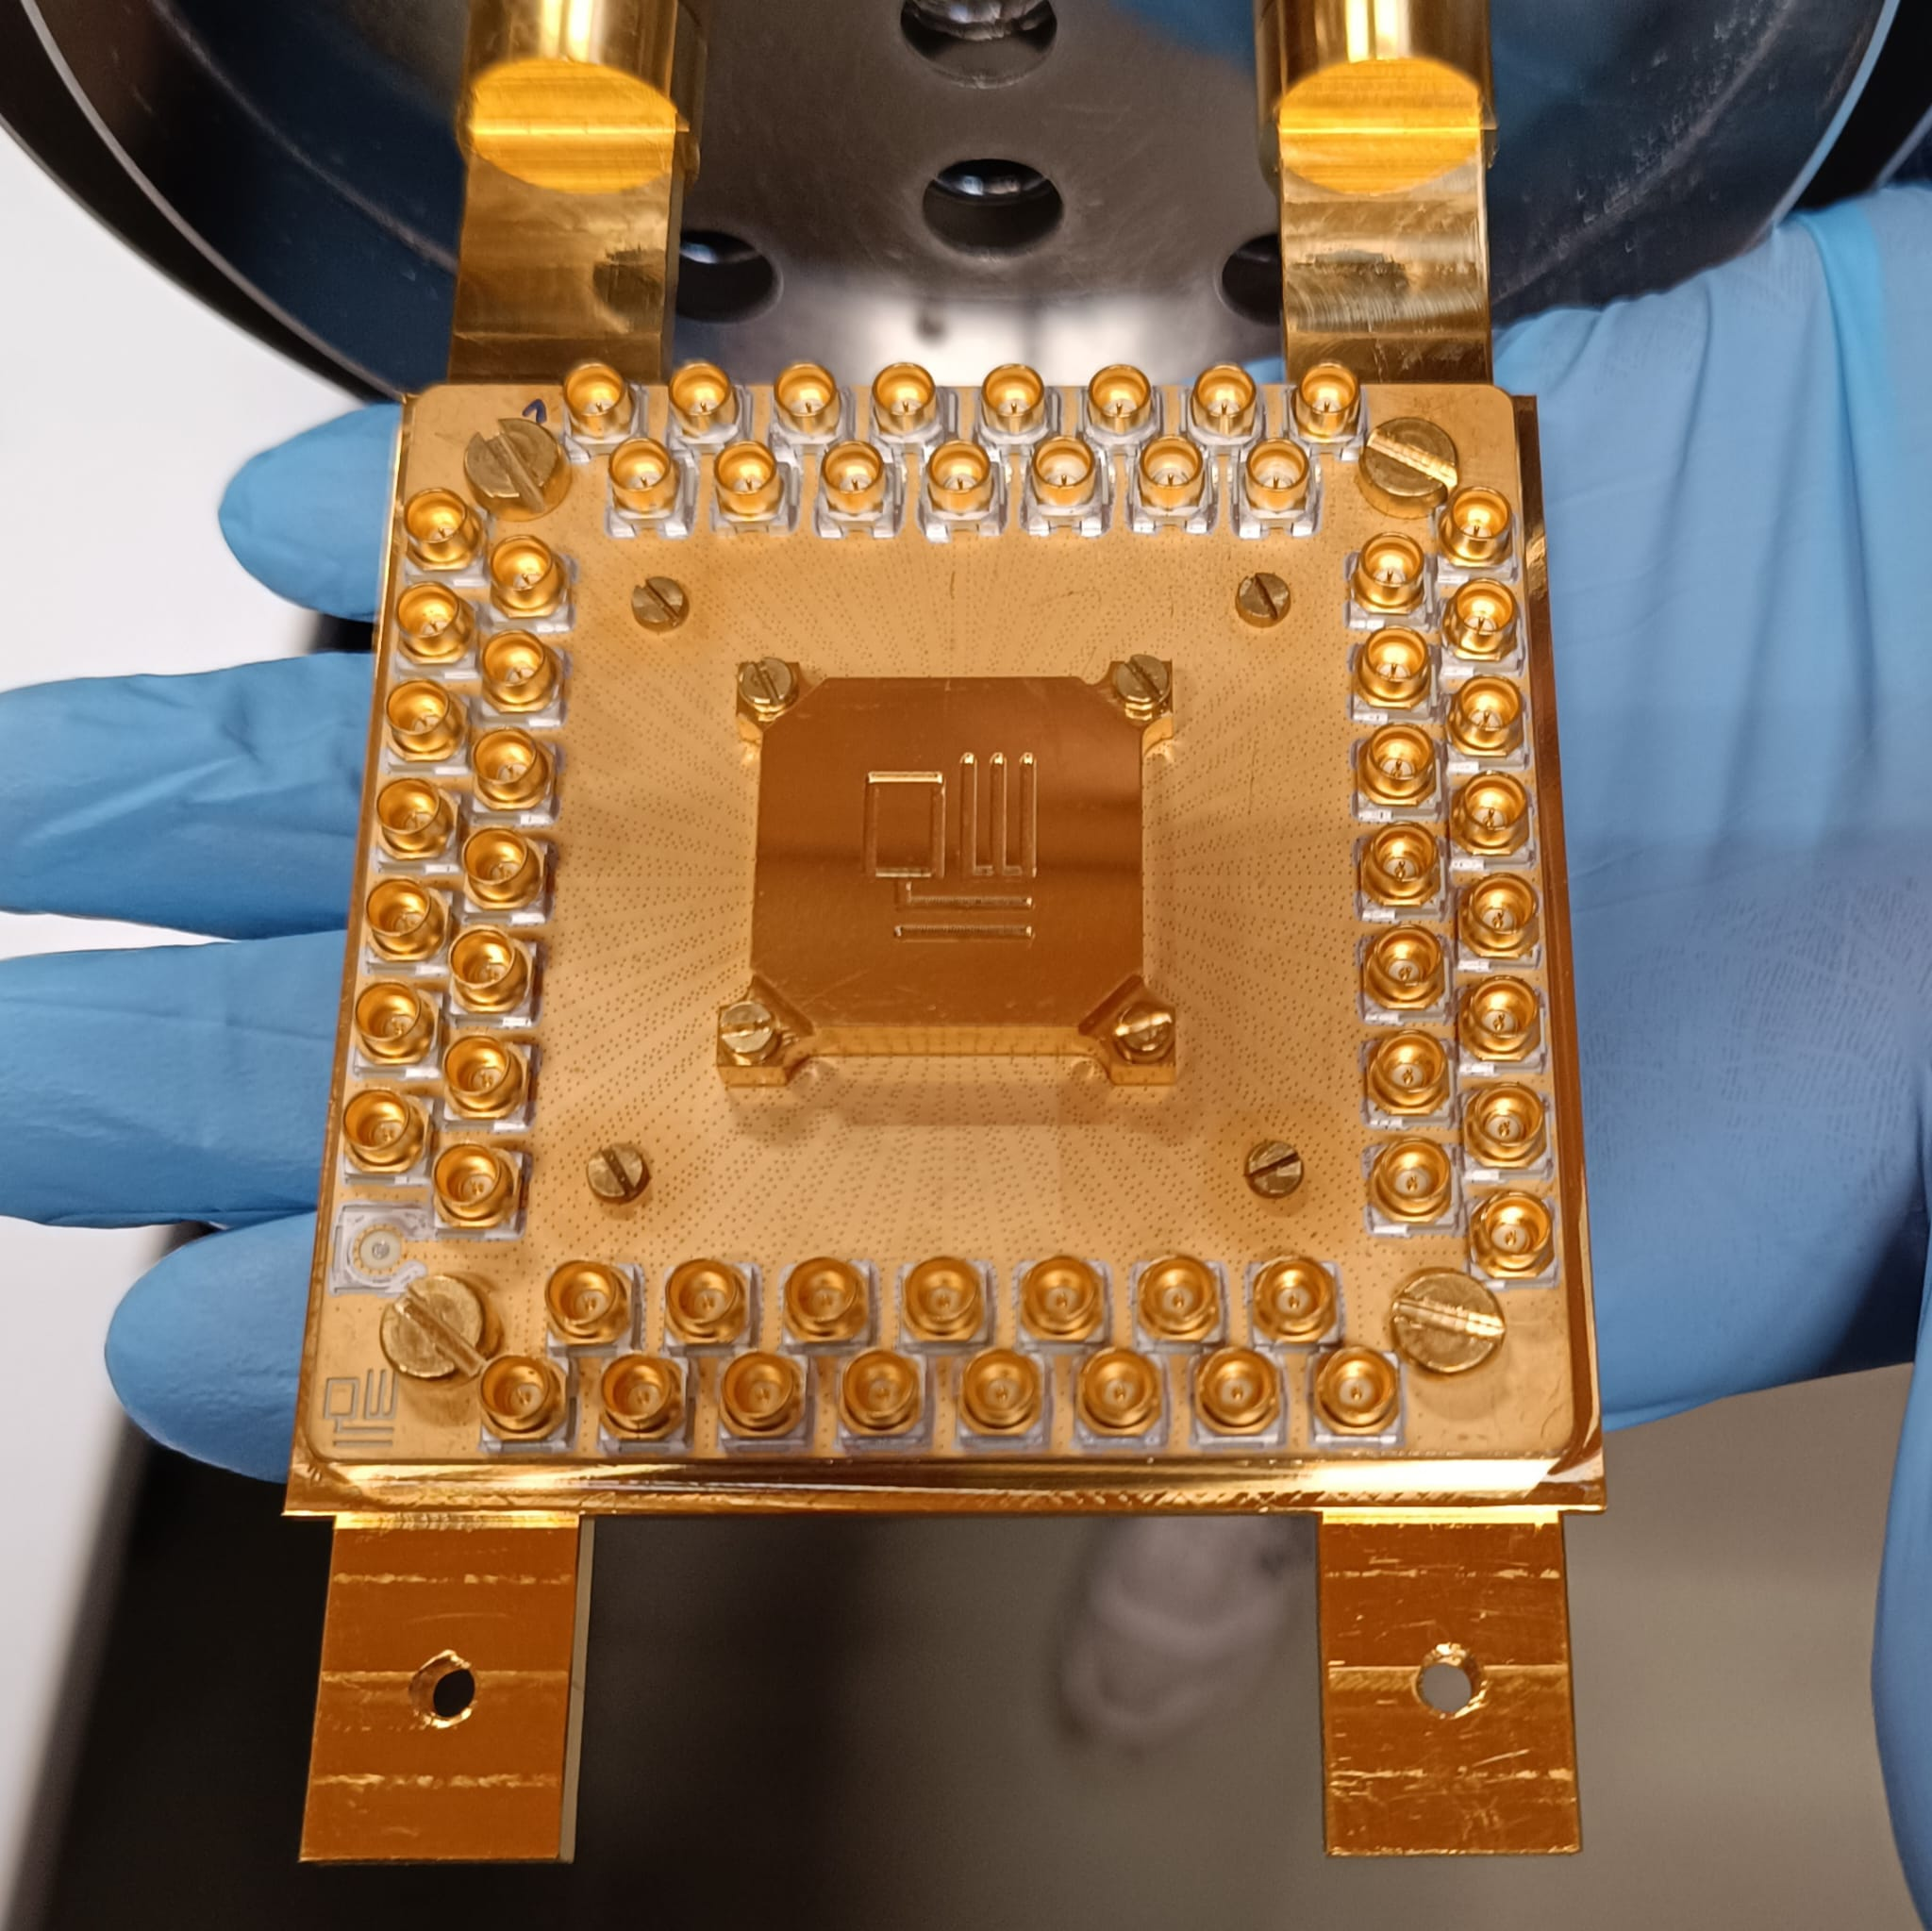
\includegraphics[width=0.80\textwidth]{figures/png/qw11q.jpeg}
        \subcaption{}
        \label{fig:qw11q_picture}
    \end{subfigure}
    \hfill
    \begin{subfigure}{0.50\textwidth}
        \centering
        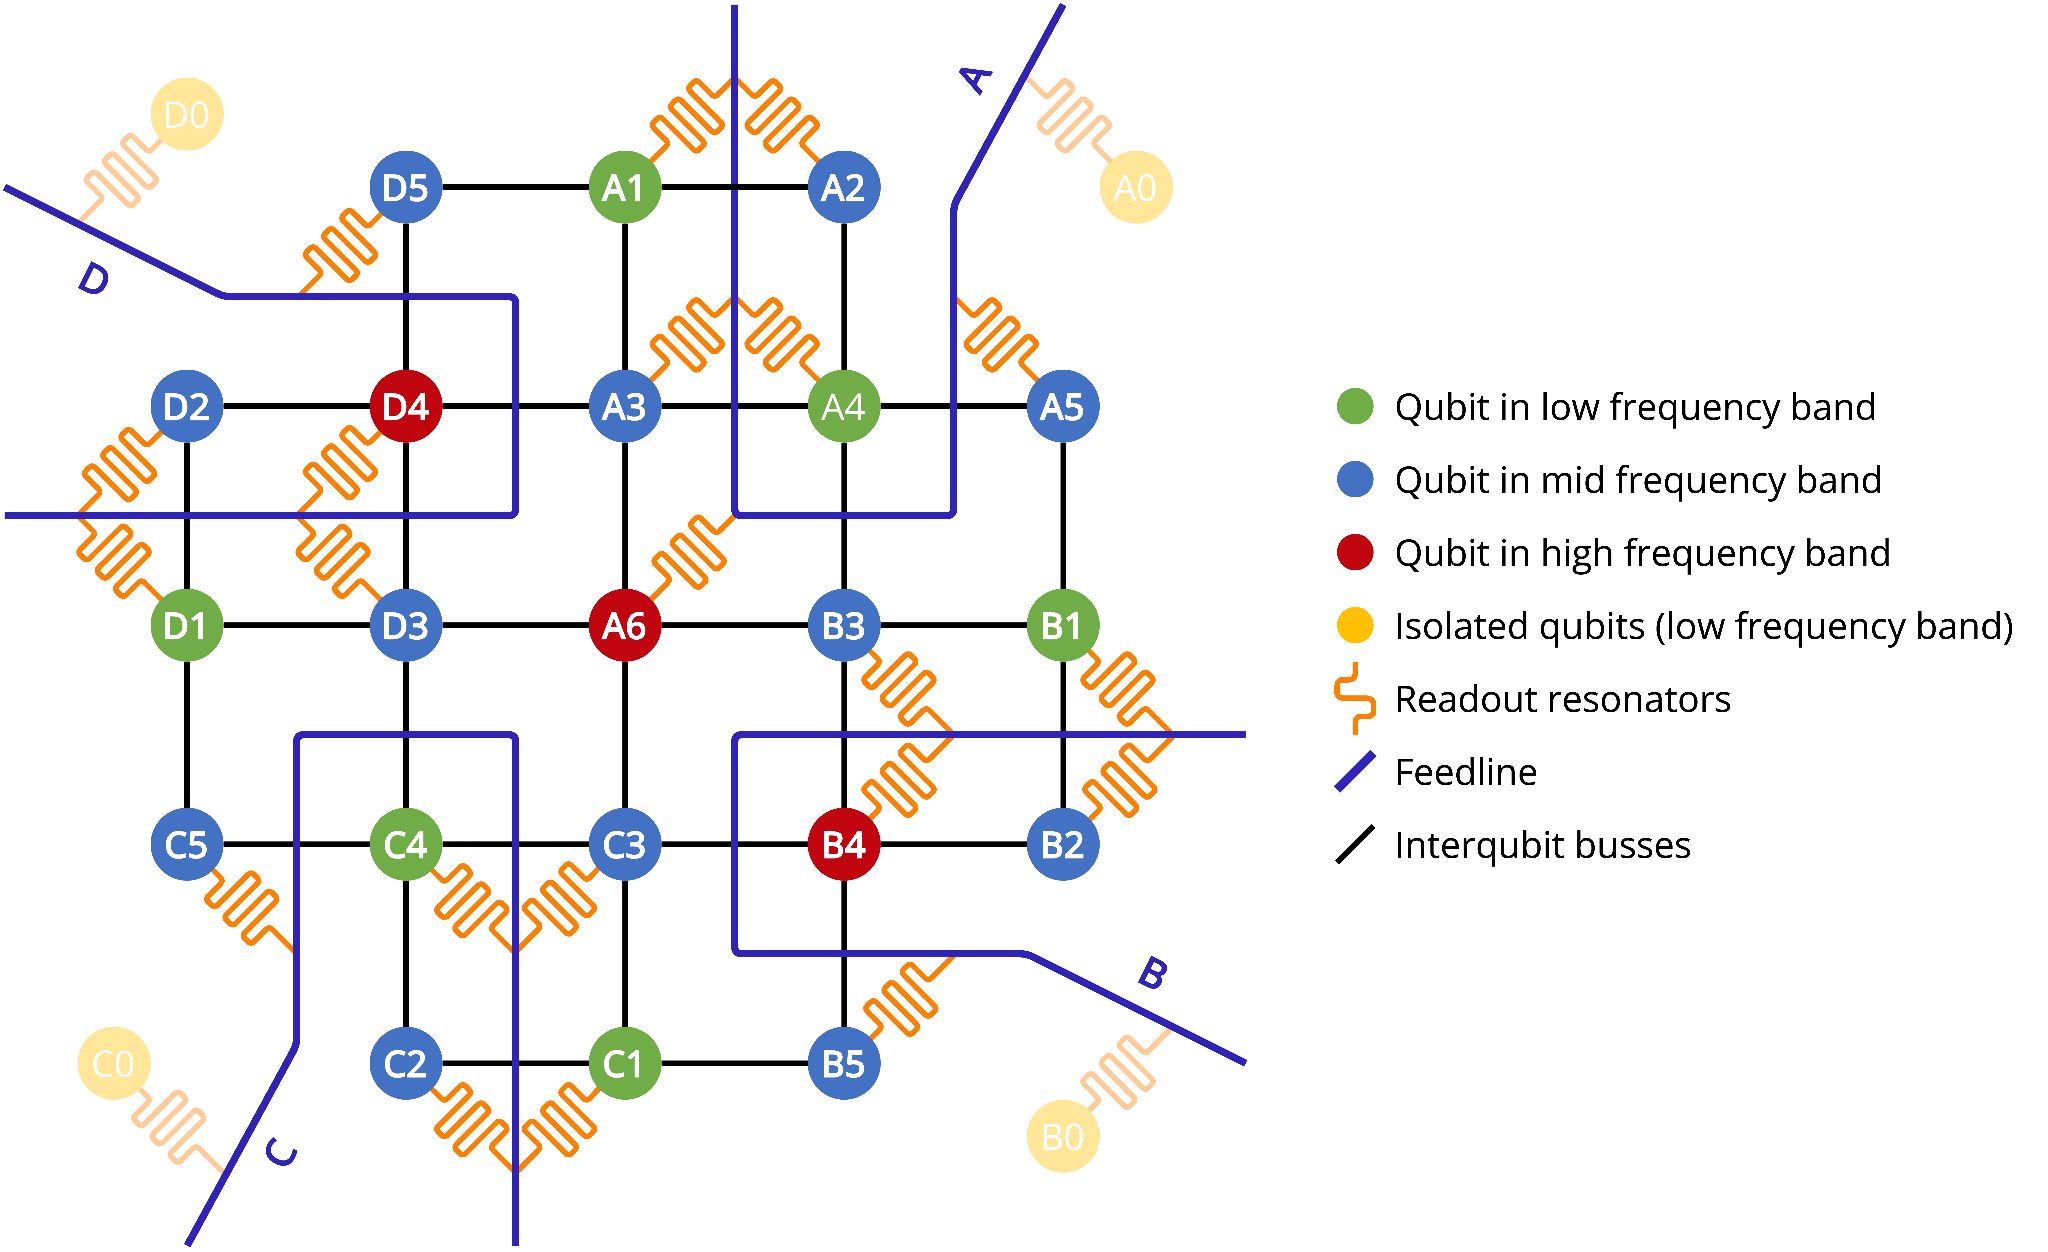
\includegraphics[width=\textwidth]{figures/png/qw11q.png}
        \subcaption{}
        \label{fig:qw11q_topology}
    \end{subfigure}
    \caption{Figure \ref{fig:qw11q_picture}: Picture of the Contralto-D chip from QuantWare. Figure \ref{fig:qw11q_topology}: Topology of the Contralto-D chip from QuantWare.}
    \label{fig:qw11q}
\end{figure}

As discussed in the previous chapter, the behavior of Josephson junctions and SQUIDs relies critically on the superconducting state of the materials involved. 
To achieve and maintain this regime, it is essential that the superconducting elements operate well below their critical temperature. 
For this reason, the Contralto-D chip is installed at the lowest temperature stage of the cryostat, where the required thermal conditions for superconductivity are met. 
This ensures the proper functioning of the quantum hardware and enables the realization of coherent quantum operations.

These systems achieve ultra-low temperatures by exploiting the unique quantum properties of helium-3 (\ce{^{3}He}) and helium-4 (\ce{^{4}He}) isotopes in a dilution process.
At the core of a dilution refrigerator is a mixing chamber, where the cooling mechanism takes place. 
When a mixture of \ce{^{3}He} and \ce{^{4}He} is cooled below approximately 870 millikelvin, the two isotopes phase-separate into a \ce{^{3}He}-rich phase and a \ce{^{3}He}-dilute phase. 
The key principle is that when \ce{^{3}He} atoms cross the phase boundary—from the concentrated phase into the dilute phase—they absorb energy from their surroundings. 
This process is endothermic and is the fundamental source of cooling in the dilution refrigerator.\\
The system operates as a closed loop: \ce{^{3}He} gas is circulated using a combination of sorption pumps and still pumps, which remove \ce{^{3}He} vapor from the still (typically at $600–800$ mK), recondense it at a higher stage, and reintroduce it into the mixing chamber. 
The refrigerator includes several thermalization stages—typically at $50$ K, $4$ K, $800$ mK, $100$ mK, and finally below $20$ mK—each connected to a corresponding cooling stage and separated by radiation shields and thermal filters to minimize heat load and noise from higher-temperature stages.
Dilution refrigerators are highly stable and capable of reaching base temperatures below $10$ mK, with hold times on the order of days or even weeks. 
These temperatures are crucial for achieving the low thermal noise and long coherence times necessary for high-fidelity quantum operations in superconducting circuits.
Specifically the cryostat employed in the lab is the XLDsl from Bluefors \cite{XLD1000}, an image of the cryostat is shown in Figure \ref{fig:XLDsl}.

\begin{figure}[h!]
    \centering
    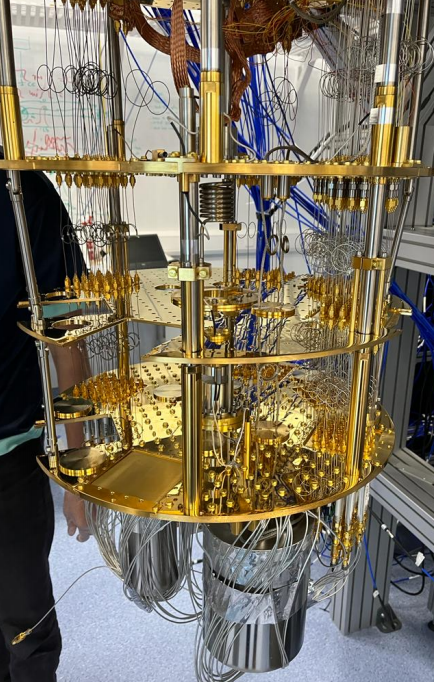
\includegraphics[width=0.35\textwidth]{figures/png/XLD1000.png}
    \caption{Picture of the XLDsl dilution refrigerator at the QRC Lab}
    \label{fig:XLDsl}
\end{figure}

Outside the cryostat, the control and readout of superconducting qubits are managed by dedicated room-temperature electronics.
These systems are responsible for generating the microwave pulses used to drive single- and two-qubit gates, as well as for acquiring and processing the output signals that encode the qubit states 
Typically they include arbitrary waveform generators (AWGs), microwave sources, mixers, digitizers, and field-programmable gate arrays (FPGAs).
The generated microwave pulses are shaped and modulated at room temperature before being attenuated and routed to the cryogenic environment. 
Similarly, signals returning from the qubits are amplified and digitized for state discrimination and further processing. 
The electronics employed in the lab for the control of the \tt{qw11q} is the OPX1000 platform by Quantum Machines \cite{opx1000}.

The software I used for the calibration of the qubits and the subsequent experiments is \Qibocal (\cite{pasquale_qibocal_2024}, \cite{qibocalscience}, \cite{qibocalgit}), while the backend for communication with the laboratory instruments is \Qibolab (\cite{efthymiou_qibolab_2024}, \cite{qibolabscience}, \cite{qibolabgit}).
\Qibolab is the control layer responsible for managing and executing low-level instructions on the hardware, bridging high-level quantum models and physical quantum platforms.
It is designed to support diverse experimental setups and allows the researcher to define custom hardware configurations through a platform abstraction and to execute custom pulse sequences using both commercial and open-source firmware.
The communication between \Qibolab and the quantum hardware is structured and modular, relying on a stack that includes instrument drivers, pulse control logic, and a compiler that translates abstract quantum gates into hardware-specific instructions.
This structure enables compatibility with heterogeneous platforms and facilitates the development of experimental drivers tailored to different laboratory environments.
\Qibocal interfaces directly with \Qibolab to apply calibration protocols on the physical device. The routines deployment takes place through the interpretation of declarative runcards written in YAML.
\Qibocal allows an easy execution of pulse sequences, collection of measurement data, and interpretation of the results through the reports that are automatically generated upon completion of the routine.

\section{Single qubit calibration experiments}

The first task that I needed to complete at the beginning of my thesis work was the calibration of at least a line of the superconducting quibts of the Contralto-D chip using the \Qibocal library.
From this point onward, for the sake of brevity, I will refer to the chip interchangeably as Contralto-D or \tt{qw11q}, which is the name of the node under which it is registered on the QRC computing cluster.
In the following I will describe the experiments that I performed and commenting on the results.

\subsection{Resonator calibration}
Before starting with the calibration of the gates necessary for quantum computing it is necessary to charachterize the qubit an clibrate the readout pulses. 
For this reason the calibration process starts with the charachterization of the resonator coupled to the qubit that will be used to perform non-destructive measurements of the qubit state.

\subsubsection{Resonator spectroscopy}
The first step to calibrate the readout pulse is to charachterize the resonator is to find the resoinator frequency, that is the tranisition frequency for the resonator. 
At this frequency, a distinct difference in the transmitted signal can be observed depending on the type of resonator used. 
In the case of a 3D cavity resonator, the signal appears amplified, whereas for a 2D planar resonator, the signal tends to be more strongly absorbed. Regardless of the resonator type, the response typically exhibits a Lorentzian-shaped peak: this peak is positive for 3D cavities due to the amplification effect, and negative for 2D resonators due to their greater absorption.

The outcome of this experiment is strongly influenced by the amplitude of the excitation pulse. 
To reliably determine the resonator frequency, the pulse duration can be fixed on the order of microseconds, which is sufficient to observe the relevant signal response.
However, selecting an appropriate amplitude requires more careful consideration. When the amplitude is high, the signal becomes more prominent, improving the signal-to-noise ratio (SNR) and making it easier to identify the resonator's response.
If the amplitude is increased too much, however, it can drive the system out of the superconducting regime.  
In this case, the resonator becomes effectively decoupled from the qubit, and the frequency observed corresponds to the so-called bare resonator frequency.
During the first calibration operations it is not necessary to have the qubit coupled to the resonator but is helpful to improve the SNR to have a more defined peak in the signal, for this reason the first calibration routines are run in a high-power regime.

In this experiment the main variables on which the experimenterer can operate are the frequency range that is willing to scan and the step of the scan. 
Regarding the frequency range a very wide scan can be useful if nothing is known about the studied resonator, but usually the design parameters are provided by the produttore; t is possible that they are not exact, but can give an idea of the region to scan.
Regarding the step for the scan, usually a step of 200 MHz can be used to probe the resonator frequency but can be reduced if a more precise scan is needed. 
An example of measurement of the bare resonator frequency is shown in Figure \ref{fig:res_high}.
 
\begin{figure}[h!]
    \centering
    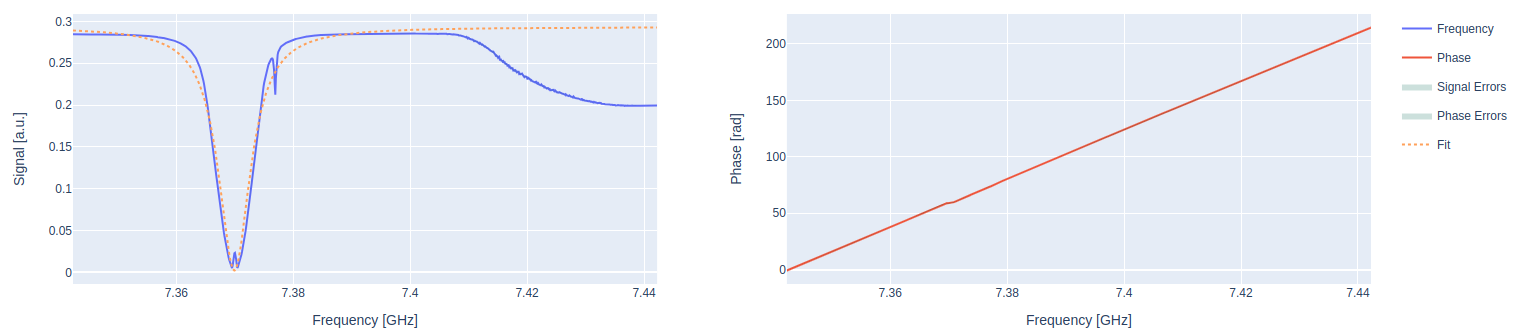
\includegraphics[width=\textwidth]{figures/png/res_spectroscopy_high.png}
    \caption{Output of resonator spectroscopy with high power on qubit B2.}
    \label{fig:res_high}
\end{figure}

An example of the measurement of the resonator frequency in the low-power regime is shown in Figure \ref{fig:res_low}.

\begin{figure}[h!]
    \centering
    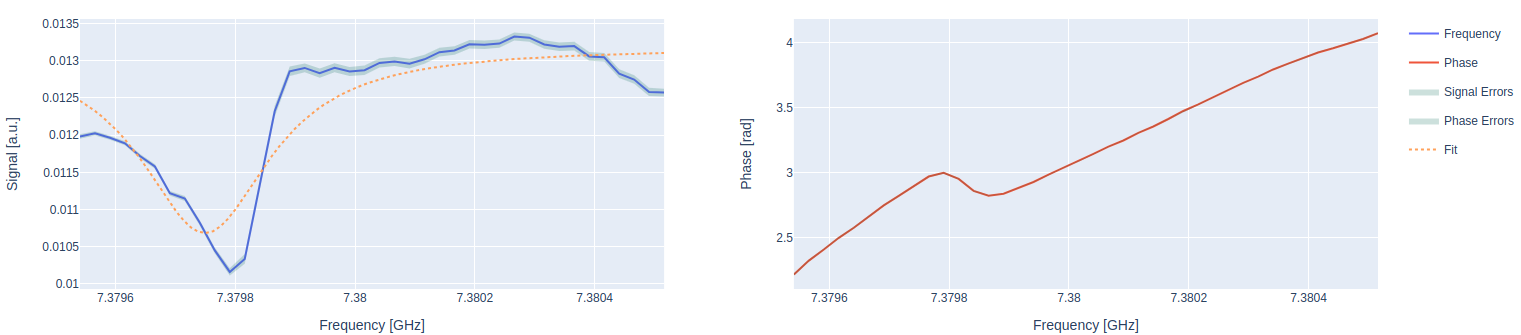
\includegraphics[width=\textwidth]{figures/png/res_low.png}
    \caption{Output of resonator spectroscopy with low power on qubit B2.}
    \label{fig:res_low}
\end{figure}

Uno studio più preciso della risposta del risonatore può essere realizzato eseguendo la routine di resonator spectroscopy cambiando la funzione di fit,  questa variazione dell'esperimento è descritta nell'appendice \hyperref[app:AppendixA]{Appendix A}

\subsubsection{Resonator punchout}
After having found the bare resonator frequency it is necessary to identify the resonator frequency under qubit coupling. 
To do this it is possible to repeat the spectroscopy, this time over a narrower frequency range and for varying pulse amplitudes. 
The resonator frequency is expected to depend strongly on amplitude: it remains constant in the high-power regime, shifts during an intermediate transition phase, and stabilizes again at a different value once the qubit-resonator interaction becomes significant.
For this calibration protocol the experimenterer must carefully choose the frequency and amplitude range to scan to avoid extremly long experiments, at the same time the frequency and amplitude steps must be small enough to clearly identify the frequency and amplitude in which the shift happens.   

%The expected result from a resonator punchout experiment is shown in Figure \ref{fig:res_punchout}
%\begin{figure}[h!]
%    \centering
%    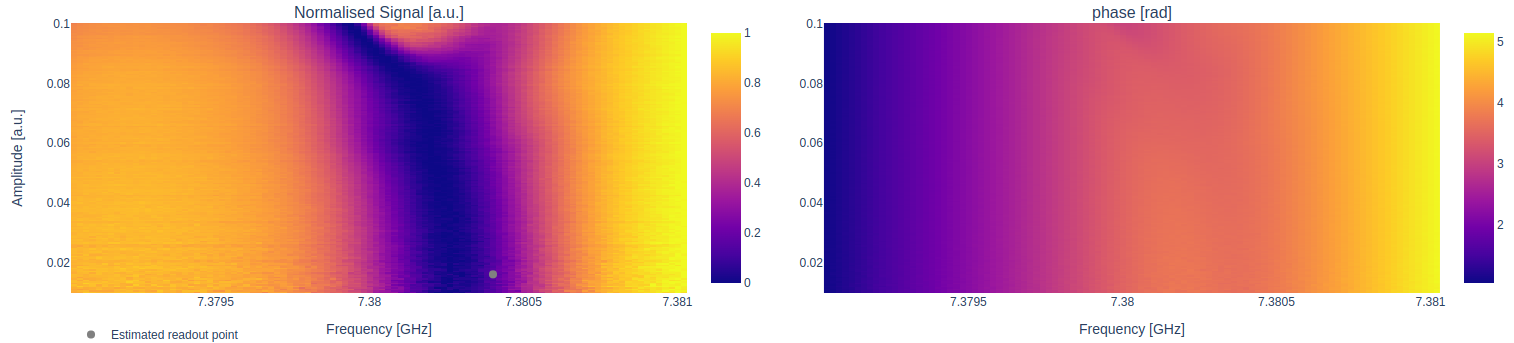
\includegraphics[width=\textwidth]{figures/png/res_punchout.png}
%    \caption{Output of resonator punchout on qubit B2.}
%    \label{fig:res_punchout}
%\end{figure}

\subsubsection{Resonator flux dependence}
As explained in section \ref{subsec:flux_tunable_transmon} it is suggested to work at the qubit sweetspot, where the qubit frequency is less sensitive to magnetic flux fluctuations.
For this reason, it is useful to estimate the location of the sweet spot prior to performing qubit spectroscopy, enabling measurements to be carried out near the optimal bias point. 
This can be accomplished by exploiting the qubit–resonator coupling: since the qubit frequency depends on the magnetic flux, as shown in equation \ref{eq:freqdepndenceonflux}, and the qubit is coupled to the resonator, the resonator frequency also exhibits a flux dependence. 
The resonator detuning in the transmon regime ($E_J \gg E_C$) can be computed as 
\begin{equation}\label{eq:resonator_flux_dependence}
    f_r(\Phi) = f_r^{\text{bare}} + \frac{g^2 \sqrt[4]{d^2 + (1 - d^2) \cos^2 \left( \pi \frac{\Phi}{\Phi_0} \right)}}{f_r^{\text{bare}} - f_q(\Phi)},
\end{equation}
where $f_r^{\text{bare}}$ is the bare resonator frequency, $g^2$ is the coupling between the transmon and the resonator, $d$ is the junctions asymmetry, $E_C$ is the charging energy, $E_J$ the Josephson energy and $\Phi_0 = h/2e$ is the flux quanta.

In \Qibocal it is possible to perform a resonator flux dependence experiment to measure and fit and the curve described by Eq. \ref{eq:resonator_flux_dependence}.
With this routine the experimenter performs a scan of the both the external bias and frequency, thihs experiment provides an approximate indication of the sweetspot.
An example of the output of this experiment is shown in Figure

%\begin{figure}[h!]
%    \centering
%    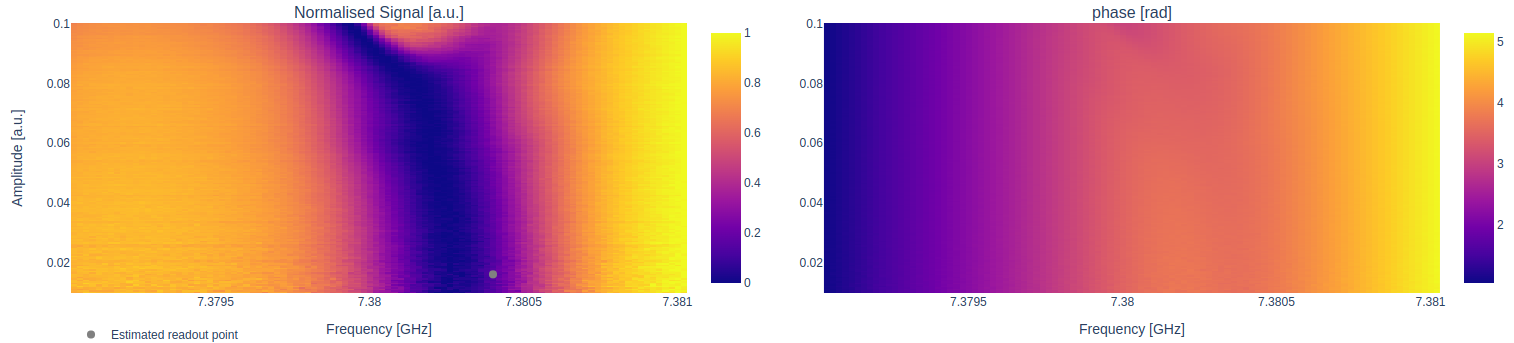
\includegraphics[width=\textwidth]{figures/png/res_punchout.png}
%    \caption{Output of resonator punchout on qubit B2.}
%    \label{fig:res_punchout}
%\end{figure}

\subsection{Qubit calibration}
After having determined all the readout parameters it is possibile to continue the calibration process by calibrating the qubit.

\subsubsection{Qubit spectroscopy}
To determine the resonance frequency of a qubit, a qubit spectroscopy experiment is performed, which, unlike resonator spectroscopy, requires a two-tone approach. 
While resonator spectroscopy is typically a single-tone measurement used to identify the resonator's response, qubit spectroscopy involves applying a drive tone to the qubit followed by a readout tone to detect the qubit state. 
This method becomes essential after an initial estimate of the readout frequency and amplitude has been obtained from a resonator punchout experiment. 
In this protocol, a drive pulse of variable frequency $\omega$ is sent through the qubit drive line. 
If the drive frequency is far detuned from the qubit transition frequency $\omega_{q}$, it will have no appreciable effect on the qubit state, and the measured signal will remain unchanged. 
However, as $\omega$ approaches $\omega_{01}$ the drive pulse can induce transitions between the qubit states. 
This excitation modifies the qubit population and, consequently, the resonator response, which is sensitive to the qubit state due to their dispersive coupling. 
When the drive frequency is near resonance and the pulse is sufficiently long, the qubit may reach a maximally mixed state leading to a detectable change in the readout signal amplitude. 
By sweeping the drive frequency and recording the corresponding readout amplitudes, one can plot a spectroscopy curve that reveals a Lorentzian dip or peak centered at the qubit transition frequency—opposite in direction to the Lorentzian feature observed in the resonator spectroscopy, due to the nature of the state-dependent dispersive shift.

An example of the output of qubit spectroscopy experiment is shown in Figure \ref{fig:qubit_spectroscopy}
\begin{figure}[h!]
    \centering
    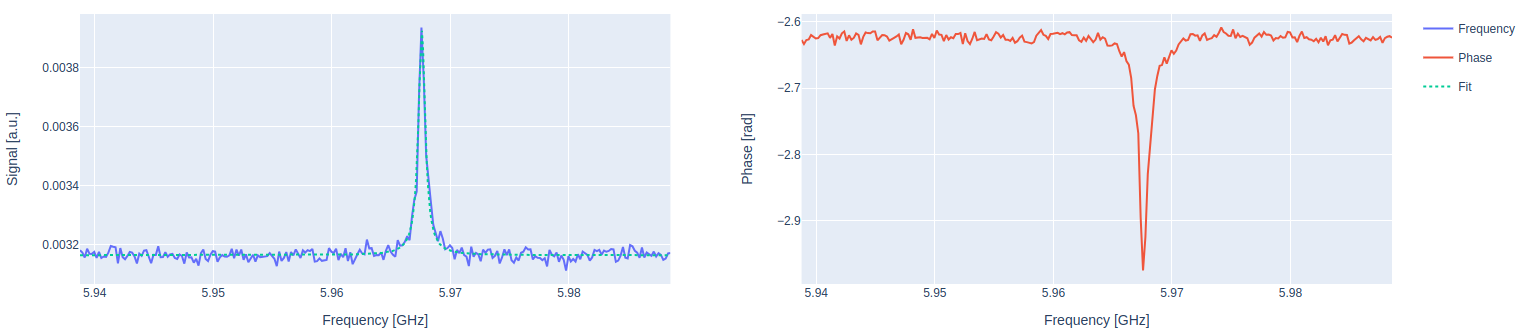
\includegraphics[width=\textwidth]{figures/png/qubit_spectroscopy.png}
    \caption{Output of qubit spectroscopy on qubit B2.}
    \label{fig:qubit_spectroscopy}
\end{figure}

\subsubsection{Qubit EF spectroscopy}
Qubit spectroscopy can also be extended to probe transitions to higher excited states beyond the first excited state. 
Directly observing these higher-level transitions typically requires significantly increased drive power, which may exceed the safe operational limits of the experimental setup. 
An alternative and more controlled approach involves first preparing the qubit in state $\ket{1}$, followed by a standard spectroscopy sequence to induce the $\ket{1} \leftrightarrow \bra{2}$ transition. 

%\begin{figure}[h!]
%    \centering
%    \includegraphics[width=\textwidth]{figures/png/ef.png}
%    \caption{Output of qubit spectroscopy to identify the transition frequency between state $\ket{1}$ ($\ket{e}$) and state $\ket{f}$ (first scited state) on qubit B2.}
%    \label{fig:ef}
%\end{figure}

Note that the description of this calibration routine has been included here for the sake of clarity and continuity of exposition; however, since it requires the qubit to be in the $\ket{1}$ state at the beginning of the spectroscopy, it can only be performed after the execution of a single-shot classification (see Section \ref{subsec:single_shot}).

\subsubsection{Qubit flux dependence}
By performing a resonator flux dependence the experimenterer obtained a first estimate for the sweetspot, now by performing a qubit flux spectroscopy.
In this experiment a constant DC current signal is sent to the qubit through the flux line with voltage and amplitude fixed for the bias level and then a qubit spectroscopy is performed.
This procedure is repeated  for different bias levels and different drive frequencies.
The expected result of the routine is shown in Figure \ref{fig:qubit_flux}.

When calibrating the qubit sweetspot it is important to consider that on a superconducting qubatum chip qubits are not completely isolated systems; rather, they interact with one another through both intentional couplings (e.g capacitive or inductive couplers) and unintended cross-talk mechanisms. 
The mutual influence that qubits exert on each other's affect their effective operating parameters, particularly their flux-dependent transition frequencies.
This means that also the location of the sweetspot can be affected by the biasing of neighboring qubits, this occurs because the flux-tuning circuitry is not perfectly isolated; biasing one qubit can induce a spurious flux in nearby qubits, effectively shifting their frequency spectra and hence their sweetspots.
Consequently, calibrating each qubit in isolation may yield misleading results, therefore, to accurately determine and operate all qubits at their true sweetspots under realistic experimental conditions, it is important to perform simultaneous calibration. 
This ensures that all mutual interactions and cross-couplings are properly accounted for, leading to a more stable and predictable multi-qubit operation.

\begin{figure}[h!]
    \centering
    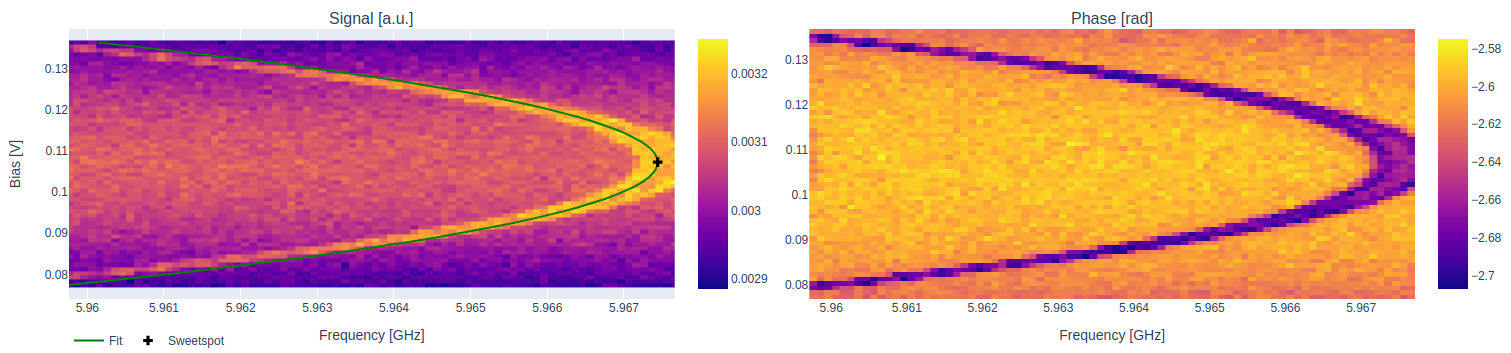
\includegraphics[width=\textwidth]{figures/png/qubit_flux.png}
    \caption{Output of the qubit flux dependence on qubit B2.}
    \label{fig:qubit_flux}
\end{figure}

\subsubsection{Qubit crosstalk}
To perform a more detailed study of the qubit crosstalk it is possible to perform a \tt{qubit\_crosstalk} experiment.

\subsection{Drive pulse calibration}

After defining all the readout parameters and the parameters for qubit control, it is necessary to calibrate the parameters of the drive pulses to be able to control rotations on the Bloch sphere.
With Rabi experiments is possibile to calibrate the drive pulses to perform precise rotations (see \cite{Rabi1936}, \cite{Wallraff2005}) within approximately $40$ ns.
This duration is typical for single-qubit gates in superconducting qubit systems, as it represents a balance between fast control and minimal spectral leakage. 
Faster gates would require higher drive amplitudes, which can increase errors due to leakage into higher transmon levels or induce unwanted transitions in nearby qubits through cross-resonance or crosstalk effects \cite{TransmonPaper}, \cite{Motzoi_2009}. 
On the other hand, significantly longer gates are more susceptible to decoherence, particularly due to $T_1$ relaxation and $T_2$ dephasing processes, which limit overall gate fidelity \cite{Barends2014-pb}.

Usually the first step of calibrating drive pulses consists in calibrating a $\pi$-pulse, namely an $X$-gate. 
The goal of the Rabi experiment is to tune the amplitude or duration of the drive pulse, in order to excite the qubit from the ground state up to state $\ket{1}$.

\subsubsection{Rabi oscillation experiments}
To experimentally probe the coherent control of a qubit in \Qibocal it is possible to perform different variations of the Rabi oscillation experiments, which provides direct evidence of the qubit's ability to undergo controlled rotations under a resonant microwave drive, as described in Section \ref{sec:qubit_control}.
In this experiment, a microwave pulse of the form  

\begin{equation}\label{eq:microwave_pulse}
    V_d(t) = A \varepsilon(t) \sin(\omega_d t + \alpha)
\end{equation}
is applied through the control line (XY line), and coupled capacitively to the qubit. 
The qubit is initialized in its ground state $\ket{0}$, and the drive frequency $\omega_d$ is set close to the qubit transition frequency $\omega_q$. 
The envelope $\varepsilon(t)$ is typically Gaussian, and its shape is kept constant throughout the experiment. 
The key parameter that is varied is the amplitude $A$ of the drive pulse (or alternatively, the duration of the pulse while keeping amplitude constant).

To better understand the evolution of the system, it is possible to consider the driven qubit in the interaction picture. 
The qubit state can be written as:
\begin{equation}\label{eq:general_state}
    \ket{\psi(t)} = C_0(t) e^{+i \omega_q t/2} \ket{0} + C_1(t) e^{-i \omega_q t/2} \ket{1}.
\end{equation}
%
Solving the time-dependent Schr\"odinger equation for state \ref{eq:general_state} under Hamiltonian\ref{eq:interaction_hamiltonian} yields the following expressions:
\begin{align}
    C_0(t) &= e^{-i \Delta_d t / 2} \left[ \cos \left( \frac{\Omega_R t}{2} \right) + i \frac{\Delta_d}{\Omega_R} \sin \left( \frac{\Omega_R t}{2} \right) \right], \\
    C_1(t) &= i \frac{\Omega}{\Omega_R} e^{i \Delta_d t / 2} \sin \left( \frac{\Omega_R t}{2} \right),
\end{align}
where $\Delta_d = \omega_q - \omega_d$ is the detuning, and
\begin{equation}
    \Omega_R = \sqrt{\Omega^2 + \Delta_d^2}
\end{equation}
is the generalized Rabi frequency.

The probability of finding the qubit in the excited state at time $t$ is given by:
\begin{equation}
    P_1(t) = |C_1(t)|^2 = \frac{\Omega^2}{\Omega^2 + \Delta_d^2} \sin^2 \left( \frac{\Omega_R t}{2} \right).
\end{equation}
This result shows that the probability oscillates in time with frequency $\Omega_R$, and the amplitude of the oscillation is reduced when the drive is off-resonant ($\Delta_d \neq 0$).
The closer the drive is to resonance, the higher the probability of full excitation.

In the resonant case, when $\omega_d =\omega_q$ and $\Delta_d = 0$ the generalized Rabi frequencyreduces to $\Omega_R = \Omega$ and the excited state probability becomes
\begin{equation}\label{eq:rabi_amplitude}
    P_e (t) = P_1(t) = \sin^2\left(\frac{\Omega t}{2} \right) = \frac{1}{2}(1-\cos(\Omega t))
\end{equation}
which is the curve that is used in the fit when performing a Rabi amplitude experiment.

An example of the output of a Rabi amplitude experiment is shown in figure \ref{fig:rabi_amplitude}.
\begin{figure}[h!]
    \centering
    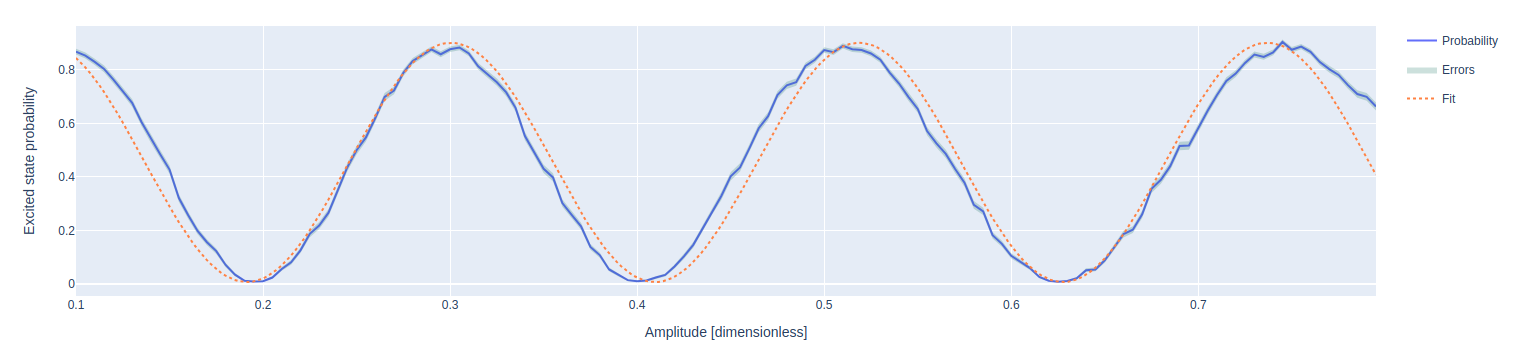
\includegraphics[width=\textwidth]{figures/png/rabi_amp.png}
    \caption{Output of the Rabi amplitude routine on qubit B2.}
    \label{fig:rabi_amplitude}
\end{figure}

A variation of the Rabi amplitude experiment consists of the Rabi length experiment, where instead of the amplitude, the parameter that is varied is the duration of the drive pulse.
The qubit is again initialized in the ground state $\ket{0}$ and subjected to a resonant microwave drive ($\omega_d = \omega_q$). 
In this case, the pulse envelope $\varepsilon(t)$ and amplitude $A$ are held constant, while the total duration of the pulse is incrementally varied. 
This enables the observation of coherent oscillations in the excited state population as a function of pulse length. 
However, unlike the idealized scenario, in realistic conditions the qubit experiences energy relaxation and dephasing, which attenuate the oscillation amplitude over time. 
To account for these effects, the excited state probability is modeled as represents the effective decay time, incorporating both energy relaxation and dephasing processes.
\begin{equation}
    P_e (t) = P_1(t)= \frac{1}{2}(1- e^{-t/\tau}\cos(\Omega_R \frac{t}{2}))
\end{equation}
where $\Omega_R$ is the generalized Rabi frequency and $\tau$ 

\begin{figure}[h!]
    \centering
    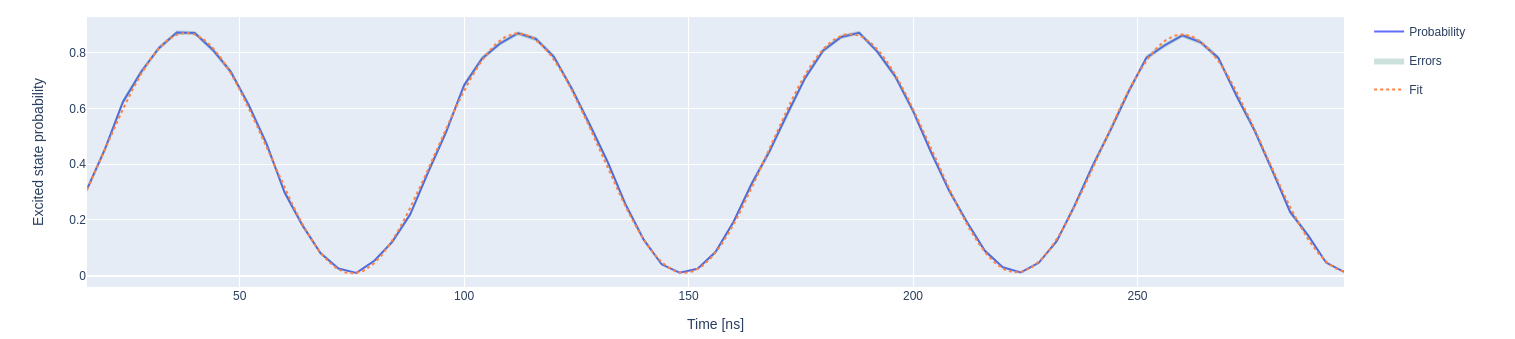
\includegraphics[width=\textwidth]{figures/png/rabi_length.png}
    \caption{Output of the Rabi length routine on qubit B2.}
    \label{fig:rabi_length}
\end{figure}

\begin{figure}[h!]
    \centering
    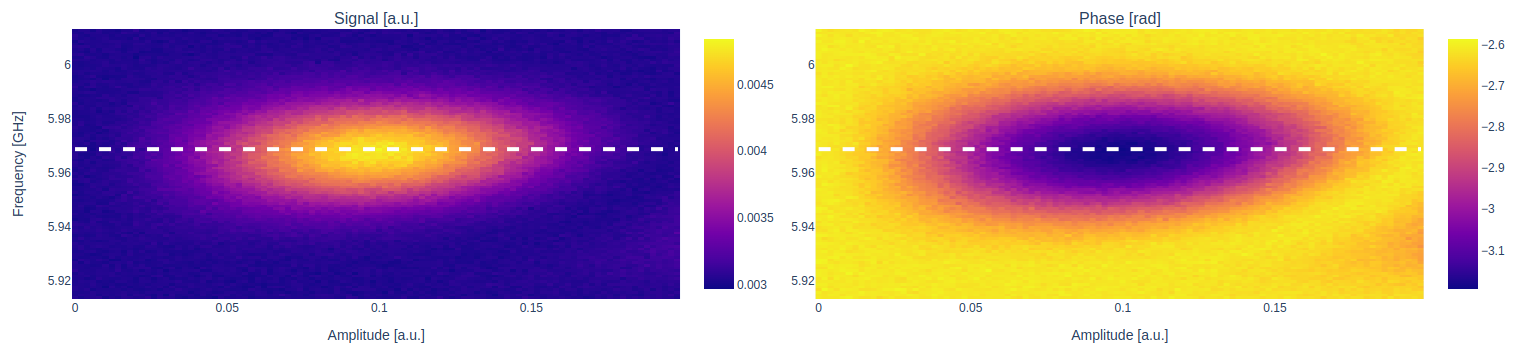
\includegraphics[width=\textwidth]{figures/png/rabi_af.png}
    \caption{Output of the Rabi amplitude-frequency routine on qubit B2.}
    \label{fig:rabi_amplitude_frequency}
\end{figure}

\subsection{Fine-tuning calibration}

\subsubsection{Ramsey experiment}\label{subsec:Ramsey}
After calibrating the readout and $\pi$-pulses, technically should be possible to execute algorithmic experiments on the qubit. 
However, essential characteristics of the qubit, such as its coherence properties and the precise drive frequency, remain to be determined; without this information, circuit fidelities would be suboptimal. 
The Ramsey experiment is a simple yet powerful protocol that allows simultaneous investigation of multiple aspects of qubit behavior, including the fine tuning of the drive frequency and verification of coherent control and signal phase consistency. 
It also enables extraction of the qubit's coherence time $T_2^*$.

In its standard implementation, the Ramsey sequence consists of two $\frac{\pi}{2}$-pulses separated by a variable delay $\tau$.\\
The first $\frac{\pi}{2}$-pulse brings the qubit from the ground state $\ket{0}$ onto the equatorial plane of the Bloch sphere, placing it in a superposition of $\ket{0}$ and $\ket{1}$.
During the delay $\tau$, he qubit state accumulates a relative phase due to its Larmor precession and environmental noise, effectively evolving around the z-axis.\\
The second $\frac{\pi}{2}$-pulse projects the final state back onto the measurement basis, and the probability of measuring the excited state $\ket{1}$ is recorded.
Repeating this procedure for different delay times $\tau$ allows to monitor the decay of coherence in the qubit state.

In the ideal, non-detuned case, where the drive frequency matches the qubit transition frequency, the observed signal exhibits a purely exponential decay toward a baseline value, from which the characteristic decoherence time $T_2^*$ can be extracted.
However, small deviations from the ideal $\frac{\pi}{2}$-pulse, due to imperfect calibration or a mismatch between the drive and quibt frequency lead to more complex behaviour.

Usually a small intentional detuning is applied, in this case the measurement outcomes show a sinusoidal modulation superimoposed on the exponential decay so that the reuslting curve can be fitted with the equation \cite{Baur2012RealizingQG}
\begin{equation}\label{eq:Ramsey}
    p_e(\tau) = \frac{1}{2} + \frac{1}{2}e^{-\tau/T_2^*}\cos{(\Delta\omega \tau)}
\end{equation}
An example of the output of a Ramsey experiment is shown in Figure \ref{fig:ramsey}

\begin{figure}[h!]
    \centering
    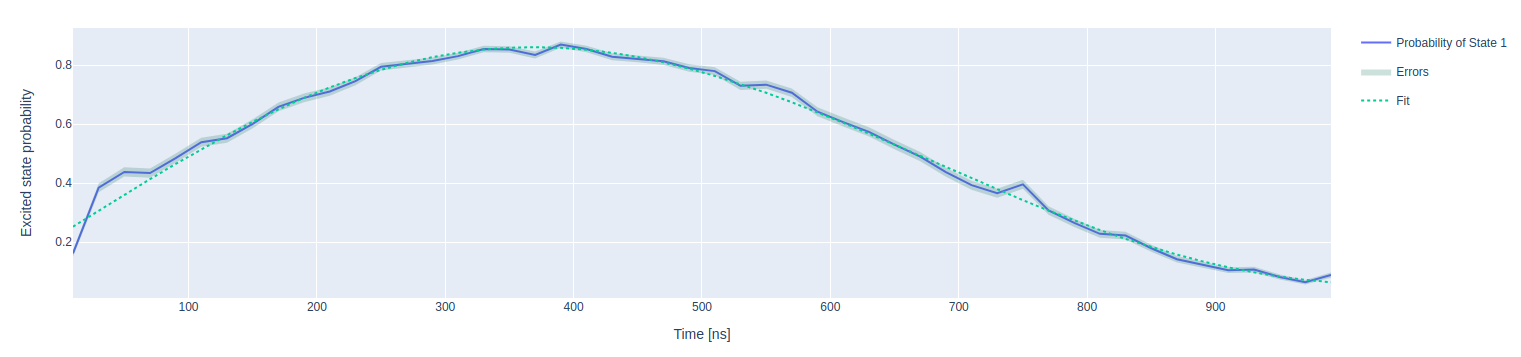
\includegraphics[width=\textwidth]{figures/png/ramsey.png}
    \caption{Output of the Ramsey amplitude routine on qubit B2.}
    \label{fig:ramsey}
\end{figure}

\subsubsection{Flipping experiment}

While the Ramsey experiment is typically used to fine-tune the drive frequency of a qubit, the Flipping experiment serves as an effective routine to calibrate the amplitude of the $\pi$-pulse, ensuring accurate implementation of $R_x(\pi)$ rotations. 
This calibration is fundamental for achieving high-fidelity gate operations, and the flipping experiment can often reveal discrepancies in the amplitude that are not evident in Rabi oscillation measurements.\\
In this protocol, a flip is defined as a pair of consecutive $\pi$-pulses, which ideally return the qubit to its initial state due to a full $2\pi$ rotation. 
The experiment begins with the qubit initialized in the ground state $\ket{0}$, followed by an $R_x(\pi/2)$ rotation that places it in an equal superposition state on the equator of the Bloch sphere. 
Without the initial $R_x(\pi/2)$ rotation, errors in the $\pi$-pulses would lead only to a global phase difference, which is not detectable via projective measurements. 
With the superposition state, however, the qubit's evolution becomes sensitive to amplitude miscalibrations, allowing over- and under-rotations to be distinguished through changes in measurement probability.

Following the initial $\pi/2$-pulse, the qubit is subjected to a number $N$ of flips choosen by the experimenter. 
After the flips, a projective measurement is performed. This procedure is repeated for increasing values of $N$, effectively building a scan of how the qubit state evolves under repeated application of imperfect $\pi$-pulses.

In the ideal case, where the $\pi$-pulse amplitude is perfectly calibrated, the repeated flips return the qubit to the equatorial plane after each cycle, resulting in a constant measurement probability. 
The recorded signal should appear as a flat line; however, if the amplitude is miscalibrated, the qubit state will drift on the Bloch sphere, leading to oscillatory behavior in the measured population as a function of the number of flips. 
This deviation is modeled by a sinusoidal function, from which the amplitude error can be quantitatively extracted.
Figure \ref{fig:flipping} shows the result of a flipping routine.

\begin{figure}[h!]
    \centering
    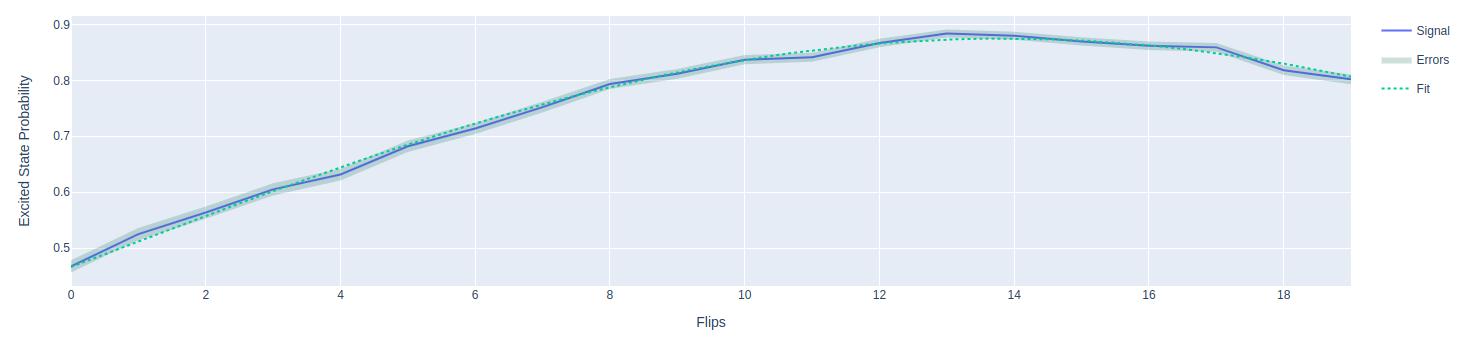
\includegraphics[width=\textwidth]{figures/png/flipping.png}
    \caption{Output of the flipping routine on qubit B2.}
    \label{fig:flipping}
\end{figure}

\subsubsection{Dispersive shift}
A possible strategy to improve the assignment fidelity is to perform a dispersive shift measurement which helps calibrate the readout frequency.
To calibrate the readout frequency based on the dispersive shift, two resonator spectroscopy measurements are performed. 
In the first, the resonator response is measured while the qubit remains in its ground state $\ket{0}$, effectively treating the system as a bare resonator. 
In the second measurement, a calibrated $\pi$-pulse is applied before each acquisition to prepare the qubit in the excited state $\ket{1}$, and the spectroscopy is repeated under otherwise identical conditions. 
The transmission or reflection spectra from both configurations are then plotted together as a function of probe frequency. 
At each frequency point, single-shot measurements are collected, and the resulting IQ data are analyzed. 
Specifically, the distance between the centroids of the two resulting IQ distributions, one corresponding to the ground state and the other to the excited state, is computed. 
The readout frequency that maximizes this centroid separation is selected, as it provides the greatest distinguishability between the two qubit states and thus optimizes the readout contrast.

A typical result for this routine is shown in Figure

\subsection{Qubit charachterization}
\subsubsection{T1 \& T2 measurement}
After having calibrated all the parameters concerning the qubit it is possible to proceed with charachterization experiments such as $T1$ and $T2$ measurements.

As explained in Section \ref{subsec:qubit_decoherence}, due to coupling to the environment the qubit in state $\ket{1}$ will decay to the state $\ket{0}$. 
To measure the charachteristic decay time $T_1$ it is possible to perform a simple experiment where the qubit is initialized in state $\ket{1}$ using a previously calibrated $\pi$ pulse.
After a variable delay $\Delta\tau$, during which the qubit undergoes spontaneous decay due to coupling to the environment, a projective measurement is performed.
For $\Delta\tau = 0$ we expect to fin the qubit in state $\ket{1}$ while for $\Delta\tau \rightarrow \infty$ the system relaxes fully to the ground state $\ket{0}$.
r intermediate times, the probability of finding the qubit in $\ket{1}$ decays exponentially, and the measured excited state population $p_e(t)$ as a function of time $t$ is fitted to the model 
\begin{equation}\label{eq:T1}
    p_e(t) = A + Be^{-\frac{t}{T_1}},
\end{equation}
where $T_1$ is the exnergy relation time and $A$, $B$ are the fitting parameters.
The expected result from this routine is shown in Figure \ref{fig:t1}.

\begin{figure}[h!]
    \centering
    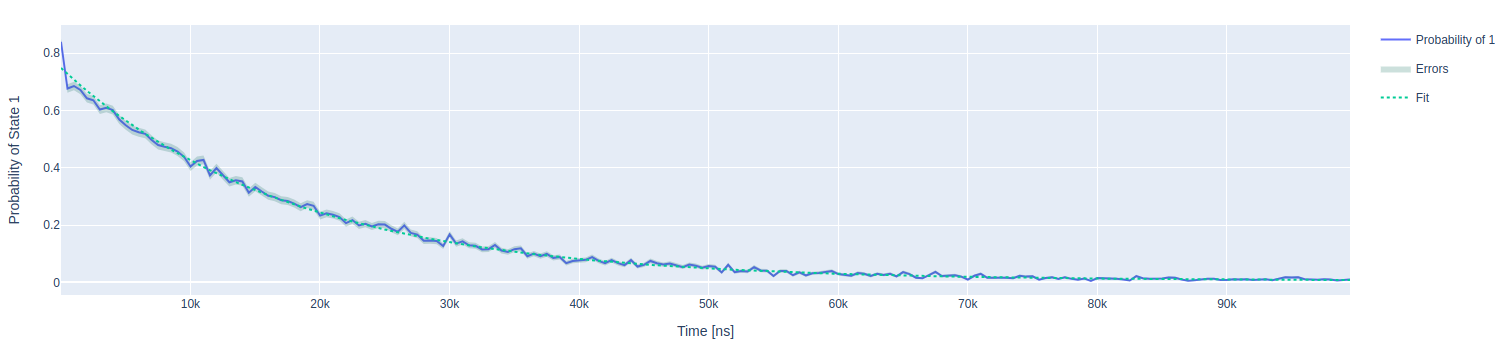
\includegraphics[width=\textwidth]{figures/png/t1.png}
    \caption{Output of the $T1$ measurement on qubit B2.}
    \label{fig:t1}
\end{figure}

After measuring $T_1$ it is necessary to measure also the dephasing time of the qubit, $T_2$; to do this in \Qibocal, it is possible to perform a T2 experiment.
The acquisition sequence of the experiment is the same as the Ramsey experiment described in Section \ref{subsec:Ramsey}: a pair of $\pi/2$-pulses is applied with a variable delay $\tau$ in between, during which the qubit freely evolves under a slightly detuned drive.
As a result, the measured excited state population exhibits oscillations in time, caused by the accumulation of phase due to the detuning. 
These oscillations are enveloped by an exponential decay that reflects the qubit’s loss of phase coherence over time.  

In the T2 experiment the same pulse sequence is used with the caveat that the drive pulse is not detuned, the protocol assumest that any error on the drive frequency has already been corrected through a Ramsey experiment.
For this reason the curve that describes the excited state population is expected to follow a simple exponential decay:
\begin{equation}
    p_e(t) = A + Be^{-\frac{t}{T_2}},
\end{equation}
where $A$ and $B$ are two fitting parameters.

\begin{figure}[h!]
    \centering
    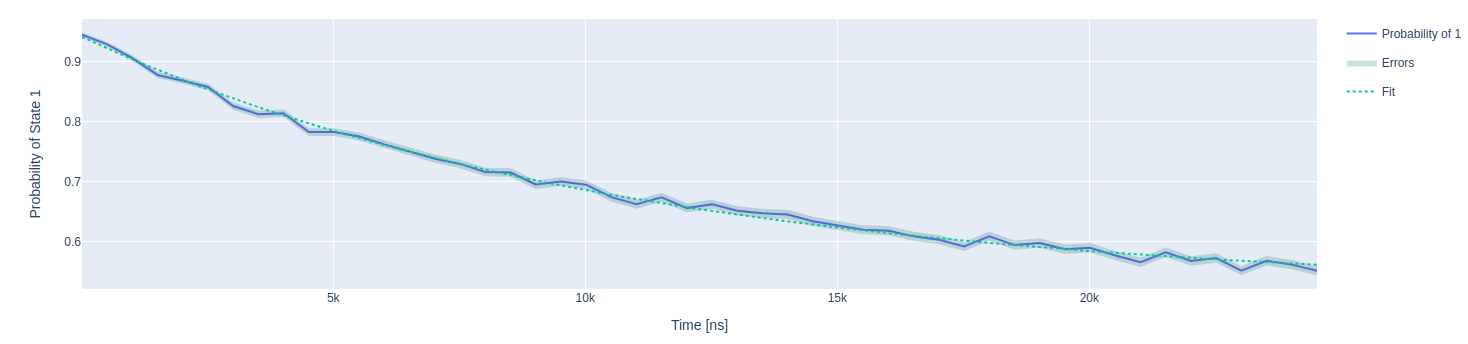
\includegraphics[width=\textwidth]{figures/png/t2.png}
    \caption{Output of the $T2$ measurement on qubit B2.}
    \label{fig:t2}
\end{figure}

\subsubsection{Single shot classification}\label{subsec:single_shot}
At this stage of the calibration procedure, the drive and measurement pulses have been individually calibrated, while a measurement now yields a clear analog output, this alone does not indicate whether the qubit was in state $\ket{0}$ or $\ket{1}$.
To establish this correspondence and enable digital state assignment, it is necessary to perform a single-shot readout experiment.

To charachterize the readout configuration of a superconducting qubit, the measurement is performed using a heterodyne detection setup (see \cite{gao_practical_2021}, \cite{krantz_quantum_2019}) which acquires the transmitted microwave signal from the readout resonator.
Although the average signal clearly distinguishes the two states, in a single instance, often called single shot, th signal is noisy. 
This noise arises both from quantum fluctuations intrinsic to the electromagnetic field inside the resonator and from added noise contributed by amplifiers and other electronics in the detection chain.
The raw signal, sampled over a finite window, is digitally integrated to produce a single complex number corresponding to one measurement instance.
Repeating this process after preparing the qubit in a known state produces a cloud of points in the complex IQ plane \cite{krantz_quantum_2019}.
For both state $\ket{0}$ and state $\ket{1}$ we typically observe one Gaussian-shaped distribution of IQ values The separation between these two clusters originates from the dispersive interaction between the qubit and the resonator, which induces a state-dependent frequency shift and consequently a distinguishable phase shift in the transmitted microwave tone. 
Since the acquisition integrates the signal over time, each shot produces a single point whose location reflects the qubit state but is blurred by noise that generates the Gaussian distributions.

The readout calibration experiment starts by preparing the qubit in state $\ket{0}$, letting it relax to its ground state and collecting IQ data without averaging.
The experiment is then repeated the after applying a $\pi$-pulse to prepare the qubit in state $\ket{1}$ and the unavaraged IQ-values are recorded.
Plotting all these single shots in the IQ plane reveals two roughly circular clusters. 

To classify the measured IQ points, the centroids of the two Gaussian-like distributions corresponding to the qubit prepared in $\ket{0}$ and $\ket{1}$ are first identified. 
The axis passing through these centroids is used to define the direction along which the state information is most distinguishable. 
The IQ plane is then rotated so that this axis aligns with the horizontal (real) axis, concentrating the relevant state-dependent variation along a single dimension. 
This rotation is characterized by an angle, measured in radians, between the centroid-connecting axis and the original $Q$-axis.

Following the rotation, the coordinate system is translated such that the centroid of the ground state distribution is placed at the origin. 
All IQ points are then projected onto the real axis, and the resulting one-dimensional distributions for each state are analyzed. 
The cumulative distribution functions of these projections are computed, and the optimal threshold is determined by finding the point that maximizes the absolute difference between the two distributions. 
This threshold defines the decision boundary used to assign a binary qubit state to any new measurement, based on its projection along the rotated axis.

The quality of the classification is then quantified by the assignment fidelity, defined as \cite{gao_practical_2021} 
\begin{equation}
    \mathcal{F} = \ -\frac{1}{2}((P(0,1)+P(1,0)))
\end{equation}
where $P(i,j)$ is the probability of measuring the qubit in state $i$ but prepared in state $j$; this fidelity is typically expected to exceed 90–95\% for a well-calibrated readout. 
It serves as a crucial figure of merit for the qubit, reflecting how reliably one can distinguish its quantum states in a single-shot measurement. 

The result of the classification routine should be similar to the one showed in Figure \ref{fig:classification}.

\begin{figure}[h!]
    \centering
    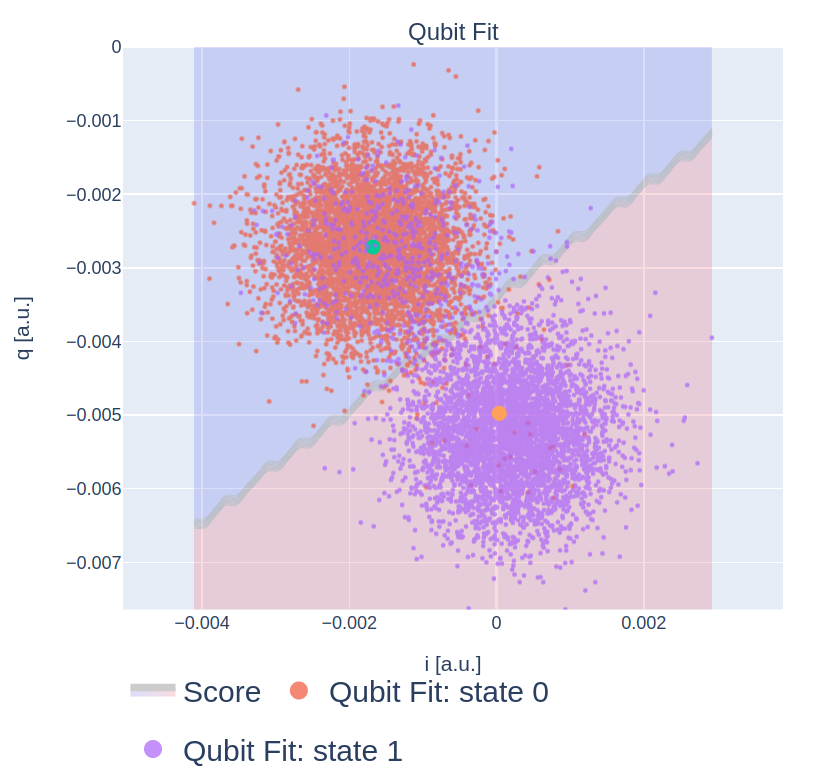
\includegraphics[width=0.4\textwidth]{figures/png/classification.png}
    \caption{Output of the single shot classification on qubit B2.}
    \label{fig:classification}
\end{figure}


\subsection{Standard Randomized Benchmarking}
The standard randomized benchmarking experiment will be described in more detail in the following chapter (see Section \ref{sec:RBsection}).
For now it is enough to say that in this routine, sequences of randomly selected Clifford gates are applied to the qubit, followed by an inverting gate that ideally returns the system to its initial state. 
By measuring the survival probability as a function of sequence length and fitting the decay curve, an estimate of the average gate fidelity is obtained.


\subsection{DRAG experiment}\label{sec:DRAG}
\subsubsection{DRAG pulse shape}
As mentioned in section \ref{sec:qubit_control}, the study of optimal pulse shapes (especially for drive and control pulses) is an active area of research. 
The Derivative Reduction by Adiabatic Gate (DRAG) technique \cite{Motzoi_2009}\cite{Gambetta_2011} is a widely used method to mitigate leakage errors during high-fidelity single-qubit gate operations.
The DRAG is the analytical solution to force the interaction Hamiltonian of the system \ref{eq:interaction_hamiltonian} to be restricted to the computational space.

The DRAG scheme implements a single-qubit rotation by applying a shaped pulse with an envelope $\Omega(t)$ on one quadrature (typically along $\hat{\sigma_x}$) and a secondary pulse with an envelope proportional to the time derivative $\dot{\Omega}(t)$ on the orthogonal quadrature (typically $\hat{\sigma_y}$).
For instance, a rotation about the $x$-axis is generated by the time-dependent Hamiltonian\cite{manenti_quantum_2023}:
\begin{equation}\label{eq:DRAG_hamiiltonian}
    \hat{H}_d(t) = \hbar \, \Omega_x(t) \sin(\omega_d t) \, \hat{\sigma}_x + \hbar \, \Omega_y(t) \sin(\omega_d t + 2\pi) \, \hat{\sigma}_y,
\end{equation}
where the pulse shapes are defined as:
\begin{align}
    \Omega_x(t) &= \Omega_0 e^{-t^2 / (2\sigma^2)}, \\
    \Omega_y(t) &= \lambda_\eta \frac{d}{dt} \Omega_x(t),
\end{align}
where $\eta$ represents the qubit anharmonicity and $\lambda$ is a dimensionless scaling parameter.
The efficacy of the DRAG correction arises from its ability to suppress virtual transitions that occur due to the spectral overlap of the primary pulse with off-resonant transitions in the multilevel qubit structure.

Theory predicts that setting $\lambda=1$ minimizes the leakage to higher excited stats, while $\lambda=0.5$ is optimal for correcting phase distortions induced during the gates \cite{Motzoi_2009}, \cite{Gambetta_2011}, \cite{Motzoi2013}.
In experimental implementations, the optimal value of $\lambda$ may deviate from theoretical predictions due to pulse distortions, limited bandwidth of the control electronics, and interactions with the readout resonator \cite{PhysRevA.82.040305}.

\subsubsection{DRAG protocol}
A straightforward experiment implemented in \Qibocal to calibrate the $\lambda$ parameter involves performing two separates measurments using DRAG pulses in the pulse sequence.
In the first experiment, a sequence of DRAG pulses is applied in the order $Y_{\pi}$$X_{\frac{\pi}{2}}$ with both pulses parametrized by a given value of $\lambda$. 
For the second measurement the procedure is the same but the pulse order is reversed $X_{\pi}$$Y_{\frac{\pi}{2}}$.
These specific sequences are chosen because they ideally result in the same final quantum state—any discrepancy between the two indicates phase misalignment, in particular these sequences exhibit opposite signs of phase errors, as explained in \cite{reed2013entanglementquantumerrorcorrection}. 

The post-processing consist in measuring the probability of the qubit being in the state $\ket{1}$ for each value of $\lambda$. 
A linear fit is performed for both pulse sequences, and the correct $\lambda$ is the value where the two lines cross. 
This intersection corresponds to the $\lambda$ value that minimizes phase errors and ensures the qubit operates with minimal distortion.

An example of the expected output for the DRAG routine is shown in Figure \ref{fig:drag}
\begin{figure}[h!]
    \centering
    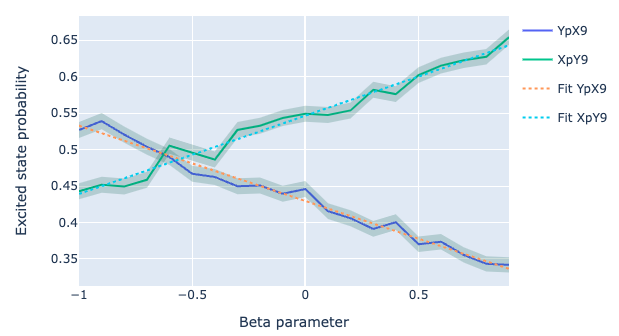
\includegraphics[width=0.65\textwidth]{figures/png/drag_simple.png}
    \caption{Expected output of the DRAG routine. $\beta$ is the symbol used in \Qibocal for the $\lambda$ parameter.}
    \label{fig:drag}
\end{figure}

%results
\chapter{RB fidelity optimization}
The calibration procedure described in Section \ref{sec:calibration} is typically time-consuming and demands significant experimental expertise, particularly when aiming for state-of-the-art performance. 
In the work presented in the previous chapter, the calibration process began from a pre-existing, even if suboptimal, configuration. 
The goal was to enhance the quality of single-qubit gates using the available \Qibocal protocols.

Even under these overall favorable initial conditions, the effort required to refine gate performance showed the limitations of manual calibration approaches. 
As quantum processors scale in both qubit count and architectural complexity, calibration becomes increasingly difficult. 
Frequent recalibrations are necessary to mitigate the effects of parameter drift and environmental fluctuations, especially in superconducting qubit platforms \cite{krantz_quantum_2019}.

Furthermore, as gate fidelities approach the fault-tolerance threshold, accurate control of gates becomes critical for most practical quantum computing applications. 
In this context, it is useful to introduce, in addition to native single-qubit gates—such as $RX_{\pi/2}$ pulses or virtual $RZ$ rotations, which are directly calibrated and implemented with a single pulse, the Clifford gates are typically composed of multiple native gates. 
Standard randomized benchmarking (RB) protocols, as used in this chapter, measure the average fidelity of a single-qubit Clifford gate. 
While this quantity does not directly reflect the fidelity of individual native gates, it remains a meaningful and widely used figure of merit. 
Because single-qubit Clifford gates form a finite subgroup of unitary operations that map Pauli operators onto themselves under conjugation and they provide a useful tool to characterize gate performance. 
Their structured algebra and invariance properties make them particularly suitable for randomized benchmarking protocols, where they enable depolarization of coherent errors and allow for SPAM-robust estimation of average gate fidelity \cite{knill_randomized_2008}.

In this chapter, i present an initial attempt to address the dual challenges of calibration complexity and residual gate errors. 
The goal is to find calibration procedures that are not only effective but also repeatable and accessible to non-expert users.  
Building on the approach proposed in \cite{kelly_optimal_2014}, which demonstrated that optimizing the sequence fidelity at a fixed length of randomized benchmarking (RB) can improve gate performance, we explored an automatic calibration improvement procedure based on randomized benchmarking fidelity as an optimization target.
In our implementation, the optimization is performed with respect to the $R_X$ pulse which is a native gate in \Qibolab (see Section \ref{subsec:native_gates}).
The optimization is performed by adjusting its amplitude, frequency and possibly, the multiiplicative factor of the quadrature component of the DRAG, pulse parameters.

The focus of this first study is on improving the average Clifford gate fidelity for single qubits. 
This choice was made considering the important role of these operations in quantum circuits and the relative simplicity of their control compared to multi-qubit gates.
Optimizing Clifford gate fidelity provides a practical testbed for validating the effectiveness of closed-loop optimization strategies before generalizing them to more complex gates.
The results presented in this chapter illustrate the performance of different optimization strategies applied to gate fidelity enhancement under realistic experimental conditions.

\section{Randomized Benchmarking}\label{sec:RBsection}
A strong limitation to the application of quantum computing technologies in different fields is the accumulation of errors due to the loss of coherence as more quantum gates are applied in sequence. 
One approach to characterize gate performance is quantum process tomography, which provides a full description of the quantum process under investigation. 
However, this method becomes impractical for systems with more than a few qubits, as its time complexity scales exponentially with the system size \cite{QPTomography}, and the results are highly sensitive to state preparation and measurement (SPAM) errors.

To overcome these limitations, randomized benchmarking (RB) was developed and is now widely used to estimate the average error rate for a set of quantum gates. 
The main idea is that the cumulative error resulting from the combined action of random unitary gate sequences, which are drawn uniformly from a group of unitaries according to the Haar measure \cite{Mele_2024}, behaves like a depolarizing channel \cite{Emerson_2005_RB}. 
This effectively removes the dependence on the specific structure of the noise and leads to a simple exponential decay model from which the average fidelity can be extracted.

Later improvements showed that the procedure could be further simplified by restricting the unitaries to the Clifford group and removing the requirement for sequences to be strictly self-inverting \cite{knill_randomized_2008}.
In the standard RB protocol, sequences of random Clifford gates $C_1, C_2, ..., C_m$ are followed by a final inversion gate $C_{m+1}$ which ideally returns the system to its initial state. 
In real devices, the measured survival probability provides an estimate of the average fidelity over the set of applied Clifford gates.

The standard RB procedure consists of the following steps:
\begin{enumerate}\label{routine:RB}
    \item Initialize the system in the ground state $\ket{0}$
    \item For each sequence length $m$, build a sequence of $m$ random Clifford gates $C_1, C_2, ..., C_m$
    \item Determine the inverse gate $C_{m+1}=(C_m\circ...\circ C_1)^{-1}$
    \item Measure $C_{m+1}\circ C_m \circ ...\circ C_1 \ket{0}$
\end{enumerate}
This process is repeated for different sequence lengths and random sequences.

In an ideal noiseless system, one would obtain:
\begin{equation}\label{eq:CliffordIdeal}
    C_{m+1}\circ C_m \circ ...\circ C_1 \ket{0} = (C_m\circ...\circ C_1)^{-1}\circ(C_m\circ...\circ C_1)\ket{0} = \ket{0}.
\end{equation}
However, in real systems Equation \ref{eq:CliffordIdeal} does not hold; instead randomization with Clifford gates behave as a depolarizing channel \ref{eq:depolarizing_channel} with depolarization probability $d$.\\
The observed survival probability as a function of sequence length $m$ follows the exponential decay model
\begin{equation}\label{eq:RB_decay}
    F(m) = Ap^m +B,
\end{equation}
where $1-p$ quantifies the depolarization rate, and $A$, $B$ capture SPAM contributions.\\
The depolarization probability $d$ is related to the average gate fidelity $F$ for a system with $n$ qubits through
\begin{equation}
    F = 1 - \frac{d}{2^n - 1}\label{eq:avarage_gate_fidelity},
\end{equation}
from which the average error per Clifford gate $\varepsilon_{Clifford}$ is obtained as
\begin{equation}
    \varepsilon_{Clifford} = 1 - F \label{eq:avg_error_Clifford_gate},
\end{equation}
leading to the final expression
\begin{equation}
    \varepsilon_{Clifford} = \frac{d}{2^n -1} = \frac{1-p}{1-2^{-n}}.
\end{equation}
This shows how the average error per Clifford gate is directly determined by the exponential decay rate $p$ extracted from the RB protocol.


\section{RB evaluation and optimization}
%TODO: inserire una introduzione per questa sezione

\subsection{RB evaluation parameters}\label{sec:RB_parameters}
In the results presented in the following, I employed the randomized benchmarking (RB) routine implemented in \Qibocal, an example of which is shown in Section \ref{sec:RB_calibration}. 
This routine was used consistently across all tests, with the following set of parameters: I used $1000$ unique random Clifford sequences (\texttt{num\_of\_sequences = 1000}), ensuring robust statistical reliability across different realizations of gate noise. 
Each sequence was evaluated at increasing circuit depths up to a maximum of $1000$ Clifford gates (\texttt{max\_circuit\_depth = 1000}), with the depths spaced by increments of $10$ (\texttt{delta\_clifford = 10}), resulting in benchmarking points at depths of $1, 10, 20, \ldots, 1000$. 
For each depth and random sequence, I generated only one instance (\texttt{n\_avg = 1}), meaning that each sequence was distinct and not repeated with the same gate pattern. 
Consequently, statistical averaging was achieved across the ensemble of random sequences at each depth rather than by repeating individual circuits. 
\footnote{All experiments and results presented in this chapter were performed using version 0.1 of \Qibocal. This means that the parameters used to execute the \texttt{rb\_ondevice} routine, as described above, refer specifically to version 0.1. At the time of writing, version 0.2 of \Qibocal has been released and is actively maintained. As a result, the available parameters for running the RB routine may have changed and might no longer correspond exactly to those described in this text.}

\subsection{Parametri da ottimizzare}
%TODO: descrivere anche il fatto che in realtà questo procedimento di fine tuning non è così banale e che può decisamente influenzare i risultati (spiegare come sono inizializzati i parametri per l'ottimizzazione)

The optimization procedures described in this work aim to enhance the average fidelity of a Clifford gate by minimizing its infidelity, as determined through RB experiments. 
The optimization is carried out over three control parameters: the amplitude and frequency of the microwave pulse and the DRAG correction parameter $\beta$, which modulates the second quadrature of the pulse shape. 
This closed-loop optimization approach follows a structure similar to the Optimal Randomized Benchmarking for Immediate Tune-up (ORBIT) protocol introduced in \cite{kelly_optimal_2014}, wherein the gate performance is iteratively improved based on benchmarking results.

Prior to the application of the optimization algorithm, a fine-tuning phase is performed to obtain reliable starting values for each parameter. 
This phase involves a sequence of calibration routines implemented within the \Qibocal framework.
The qubit frequency is first refined using a Ramsey experiment (see Section \ref{subsec:Ramsey}), subsequently a flipping sequence (see Section \ref{subsec:Flipping}) is used to adjust the microwave pulse amplitude to ensure that the applied drive results in a precise $\pi$-rotation.
Finally, the optimal value of the DRAG parameter $\beta$ is estimated through a dedicated DRAG calibration routine (see Section \ref{sec:DRAG}).
After each of these routines, the platform configuration is updated accordingly in the \tt{platform.json} file, which stores the relevant parameters for the experimental setup 
\footnote{In \Qibolab the \tt{qibolab.Platform} object holds all the information required to execute programs in a real QPU. It is comprised by different objects that contain information about the native gates and the lab's instrumentation. The QPU parameters can be saved in (and loaded from) the \tt{parameters.json} file.}.

These calibrated values are then used to initialize the optimization algorithm, as illustrated in the code reported in Listing \ref{snippet:params_init}.

\begin{lstlisting}[language=Python, caption={Code to set up the RX gate optimization experiment.}, label={snippet:params_init}]
    
    with Executor.open(
        "myexec",
        path=executor_path,
        platform=platform,
        targets=[target],
        update=True,
        force=True,
    ) as e:
    
        e.platform.settings.nshots = 2000
        drag_output = e.drag_tuning(beta_start=-4, beta_end=4, beta_step=0.5)
        ramsey_output = e.ramsey(
            delay_between_pulses_end=1000,
            delay_between_pulses_start=10,
            delay_between_pulses_step=10,
            detuning=3000000,
            relaxation_time=200000,
        )
        flipping_output = e.flipping(
            nflips_max=50,
            delta_amplitude=0.0005,  
            nflips_step=1,
        )
    
        beta_best = drag_output.results.betas[target]
        ampl_RX = e.platform.qubits[target].native_gates.RX.amplitude
        freq_RX = e.platform.qubits[target].native_gates.RX.frequency
    
        init_guess = np.array([ampl_RX, freq_RX, beta_best])
    
        lower_bounds = np.array([-0.5, freq_RX - 4e6, beta_best - 0.25])
        upper_bounds = np.array([0.5, freq_RX + 4e6, beta_best + 0.25])
        bounds = Bounds(lower_bounds, upper_bounds)
    
        opt_results, optimization_history = rb_optimization(
            e, target, method, init_guess, bounds
        )
    
    report(e.path, e.history)
    
\end{lstlisting}

In addition to defining the initial parameter values, explicit boundaries were also set for the optimization. 
This choice was motivated by the need to constrain the search space to physically meaningful regions, avoid unstable pulse configurations, and ensure compatibility with the dynamic range and resolution of the control electronics.
For the amplitude, the range was chosen to match the full extent accessible by the hardware. 
The frequency parameter, expressed in Hz, was allowed to vary within a window of 4 MHz centered on the optimal resonance frequency obtained from the Ramsey experiment, ensuring that only physically meaningful detunings are explored. 
For the DRAG parameter $\beta$, the search range was set to $0.25$ around the value returned by the initial DRAG calibration; this interval corresponds to the resolution used in the scan performed during the \tt{drag} routine, thus preserving consistency with earlier characterization steps.

In a subsequent phase of this study, a comparative analysis was performed by repeating the optimization while keeping the pulse shape fixed to a Gaussian envelope, effectively removing $\beta$ as an optimization variable. 

%TODO: try to run at least once the NM from not-fine tuned

\section{SciPy optimization methods}\label{Sec:OptimizationMethods}

\subsection{Nelder-Mead}
The initial optimization attempts were carried out using standard algorithms available in the \texttt{SciPy} library \cite{SciPy-NMeth}.
Come primo metodo di ottimizzazione è stato utilizzato un metodo che fosse gradient-free in modo tale che fosse meno sensibile al rumore delle misure. 
Nello specifico siamo partiti da Nelder-Mead il cui utilizzo per l'ottimizzazione della fidelity dell'RB era già riportata in letteratura in \cite{kelly_optimal_2014}.

\subsubsection{Algorithm information}
The Nelder-Mead optimization method, originally introduced by Nelder and Mead in 1965 \cite{NelderMeads}, is a widely used numerical optimization technique for unconstrained problems in multidimensional spaces. \\
This derivative-free method is operates using simplex, which is a polytope of $n+1$ vertices in a $n$-dimensional space.
The algorithm iteratively updates the simplex by replacing its worst-performing vertex with a new candidate point, thereby guiding the search towards an optimal solution. 
If the goal is to minimize a given function $f(\mathbf{x})$ where $\mathbf{x} \in \mathbb{R}^n$ the algorithms proceeds with the following steps:\begin{enumerate}
    \item If not otherwise initialized, $n+1$ points are sampled for building the initial symplex
    \item Order the test points according to their values at vertices: $f(\mathbf{x}_1) \leq f(\mathbf{x}_2) \leq \dots \leq f(\mathbf{x}_{n+1})$ and check whether the algorithm should terminate.
    \item Calculate $\mathbf{x}_0$, the centroid of all points except $\mathbf{x}_{n+1}$.
    \item Reflection: Compute the reflected point $\mathbf{x}_r = \mathbf{x}_0 + \alpha(\mathbf{x}_0 - \mathbf{x}_{n+1})$ with $\alpha > 0$. 
            If $\mathbf{x}_r$ satisfies $f(\mathbf{x}_1) \leq f(\mathbf{x}_r) < f(\mathbf{x}_n)$, then a new simplex is obtained by replacing the worst-performing point $\mathbf{x}_{n+1}$ with $\mathbf{x}_r$ and then go to step 1.
    \item Expansion: If $\mathbf{x_r}$ is the current best point, meaning that $f(\mathbf{x}_r) < f(\mathbf{x}_1)$, then the expanded point is computed: $\mathbf{x}_e = \mathbf{x}_0 + \gamma(\mathbf{x}_r-\mathbf{x}_0)$ with $\gamma>1$.
           If $\mathbf{x}_e$ satisfies $f(\mathbf{x}_e) < f(\mathbf{x}_r)$, then a new simplex is obtained by replacing $\mathbf{x}_{n+1}$ with the expanded point $\mathbf{x}_e$ and then go to step 1.\\
            If instead $f(\mathbf{x}_e) \geq f(\mathbf{x}_r)$, the new simplex is obtained by replacing $\mathbf{x}_{n+1}$ with $\mathbf{x}_r$, and then go to step 1.
    \item Contraction: In this case is certain that $f(\mathbf{x}_r) \geq f(\mathbf{x}_n)$ then:\begin{itemize}
        \item If $f(\mathbf{x}_r) < f(\mathbf{x}_{n+1})$: compute the contracted point $\mathbf{x}_c=\mathbf{x}_0 +\rho(\mathbf{x}_{r}-\mathbf{x}_0)$ with $0<\rho \leq 0.5$.
                If $\mathbf{x}_c$ satisfies $f(\mathbf{x}_c) < f(\mathbf{x}_{r})$, then a new simplex is obtained by replacing $\mathbf{x}_{n+1}$ with  $\mathbf{x}_c$ and go to step 1.\\
                Else go to step 6.
        \item  If $f(\mathbf{x}_r) \geq f(\mathbf{x}_{n+1})$: compute the contracted point $\mathbf{x}_c=\mathbf{x}_0 +\rho(\mathbf{x}_{n+1}-\mathbf{x}_0)$ with $0<\rho \leq 0.5$.
                If $\mathbf{x}_c$ satisfies $f(\mathbf{x}_c) < f(\mathbf{x}_{n+1})$, the a new simplex is constructed with $\mathbf{x}_c$ and go to step 1.\\
                Else go to step 6.
    \end{itemize}
    \item Shrinkage: Replace all points except the best, $\mathbf{x}_1$, with $\mathbf{x}_i = \sigma(\mathbf{x}_i - \mathbf{x}_1), 0<\sigma \leq 0.5$  
\end{enumerate}
The algorithm terminates when the standard deviation of the function values of the current simplex fall below a user-initialized tolerance. 
When the cycle stops the point of the simplex associated to the lower function value is returned as proposed optimum

The values of the parameters $\alpha, \gamma, \rho$ and $\sigma$ were left to default of \tt{SciPy}: $\alpha=1, \gamma=2, \rho=0.5, \sigma=0.5$. 

\subsubsection{Results}
In all applications of the Nelder-Mead optimization algorithm presented in this work, a maximum number of function evaluations was imposed to prevent excessively long experimental runtimes. 
The primary limitation arises from the cost function itself, which corresponds to the average gate fidelity estimated via RB. 
By using the parameters reported in Section \ref{sec:RB_parameters}, each RB sequence evaluation requires a minimum of 20 seconds, subsequently the evaluation of the cost function is particularly resource-intensive in terms of computation time.
To mitigate these constraints, both a cap on the total number of cost function evaluations and a maximum number of optimization steps were defined. 
It is important to note that each iteration of the NM algorithm typically involves the evaluation of multiple points in parameter space: at least four in the case of optimization over three parameters, and at least three when optimizing over two parameters (i.e., in a two-dimensional space).

In the first run of the algorithm, the maximum number of iterations was limited at 40 such that no more than 160 cost function evaluations were performed.
dditionally, a convergence tolerance of $1\cdot10^{-4}$ was set (\texttt{tol=1e-4} \footnote{In \texttt{scipy.optimize.minimize}, this parameter sets both the tolerance on the optimization variables, referred to as \texttt{xtol}, and the tolerance on the cost function value (\texttt{ftol}).}), applying stopping criteria to both parameter updates and cost function changes.

The results of this initial optimization attempt are shown in Figure \ref{fig:NM_plots}. As illustrated in Figure \ref{NM_true_fig:fidelity}, a clear improvement in gate fidelity was achieved, increasing from an initial value of $99.02\%$ to a final value of $99.71\%$.
Despite this apparent improvement, the optimizer did not converge within the specified tolerance. After forty steps, the stopping criterion was not satisfied, and the optimization was formally marked as unsuccessful. 
Nevertheless, the progression of the fidelity suggests a stable improvement trend, indicating that the algorithm was moving toward a local optimum even if convergence, as defined by the stopping conditions, was not strictly achieved.

\begin{figure}[h!]
    \centering
    \begin{subfigure}[t]{0.45\textwidth}
        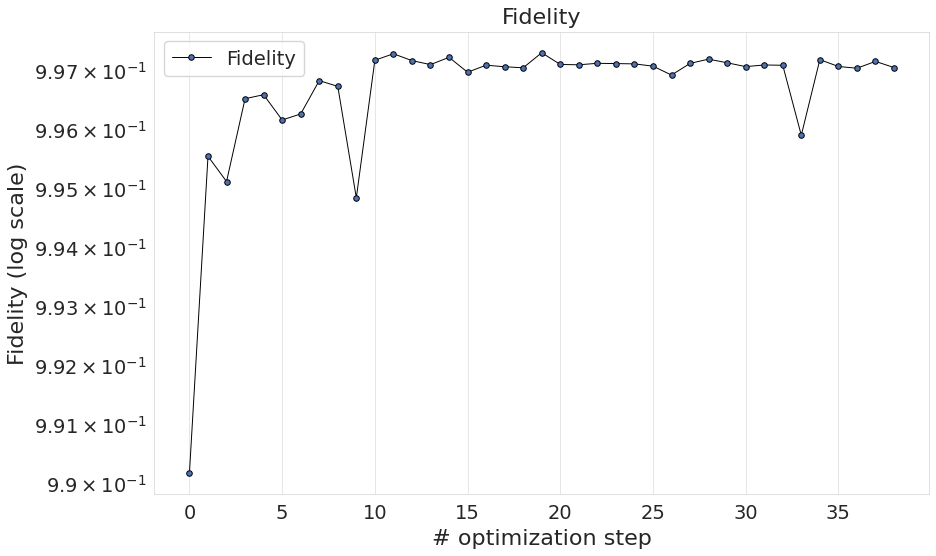
\includegraphics[width=\textwidth]{figures/png/RB_optimization/NM/post_ft_true/NM_fid.png}
        \caption{Plot of the average Clifford gate fidelity as a function of the function evaluations.}
        \label{NM_true_fig:fidelity}
    \end{subfigure}
    \hfill
    \begin{subfigure}[t]{0.45\textwidth}
        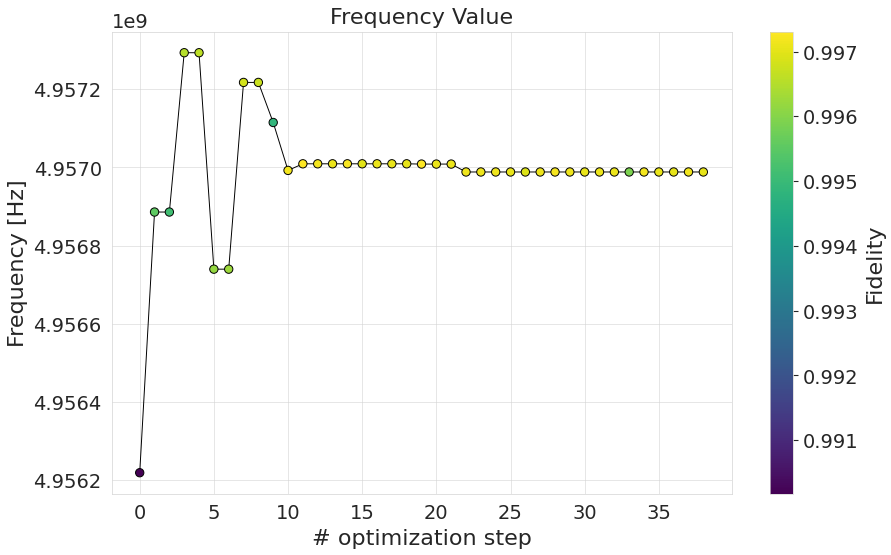
\includegraphics[width=\textwidth]{figures/png/RB_optimization/NM/post_ft_true/frequency.png}
        \caption{Plot of the frequency of the $R_X$ gate corresponding to different optimization steps.}
        \label{NM_true_fig:frequency}
    \end{subfigure}

    \vspace{0.5cm}

    \begin{subfigure}[t]{0.45\textwidth}
        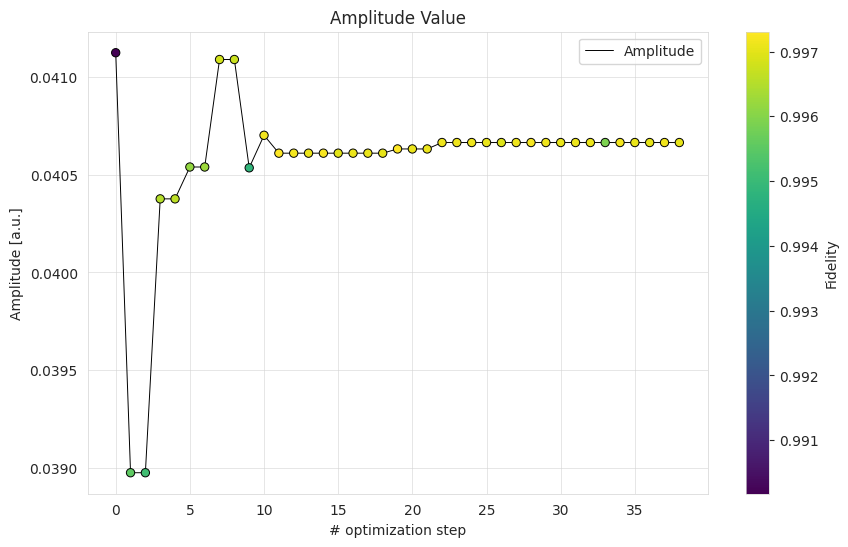
\includegraphics[width=\textwidth]{figures/png/RB_optimization/NM/post_ft_true/amplitude.png}
        \caption{Plot of the amplitude of the $R_X$ gate corresponding to different optimization steps.}
        \label{NM_true_fig:amplitude}
    \end{subfigure}
    \hfill
    \begin{subfigure}[t]{0.45\textwidth}
        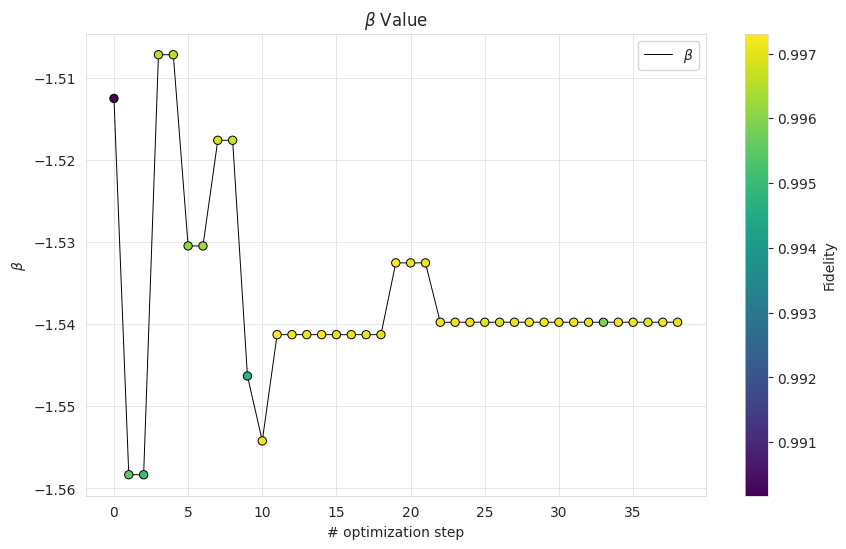
\includegraphics[width=\textwidth]{figures/png/RB_optimization/NM/post_ft_true/beta.png}
        \caption{Plot of the $\beta$ multiplying coefficient for the second quadrature component of the DRAG pulse.}
        \label{NM_true_fig:beta}
    \end{subfigure}

    \caption{Plots of the fidelity and optimization parameters as a function of the number of optimization step.}
    \label{fig:NM_plots}
\end{figure}

In Figure \ref{NM_true_fig:fidelity}, the evolution of the fidelity during the optimization is shown. 
The corresponding values of the parameters being optimized are reported in Figures \ref{NM_true_fig:frequency}, \ref{NM_true_fig:amplitude}, and \ref{NM_true_fig:beta}. 
From these plots, it is again evident that the optimization is converging (possibly to a local minimum) as the parameters stabilize around specific values: \texttt{amplitude} $= 0.04$, \texttt{frequency} $= 4.957$ GHz, and \texttt{beta} $= -1.54$.

However, a possible limitation to the performance of this optimization approach may lie in the absence of an explicitly defined initial simplex.
Setting only the initial parameter values, without specifying the full simplex, can lead the algorithm to explore the parameter space inefficiently. 
For this reason, further runs of the same method were carried out, this time also initializing the simplex explicitly.

Furthermore, considering that the allowed variation range for the $\beta$ parameter was restricted to only $\pm0.25$ around the value determined by the \tt{drag\_tuning} routine, I explored the possibility of improving the efficiency of the optimization by reducing the number of free parameters. 
Specifically, additional optimization runs were performed in which only the amplitude and frequency of the $R_X$ pulse were optimized, while $\beta$ was kept fixed.

This choice was motivated by the working assumption that, at least in this initial phase, leakage errors were not the dominant source of infidelity. 
Since the DRAG correction primarily addresses leakage to higher energy levels, it was hypothesized that optimizing $\beta$ would have a limited effect on the overall gate fidelity compared to the more significant impact of accurately calibrating the native gate's amplitude and frequency. 
As such, the focus was placed on parameters expected to yield the greatest improvements in fidelity while maintaining a limited run time.

Some optimization runs were performed with this nrevised configuration.
The results of these runs are reported in the following sections and are labeled as \tt{init\_symp\_1}, \tt{init\_symp\_2}, and \tt{init\_symp\_3}.

\begin{figure}[h!]
    \centering
    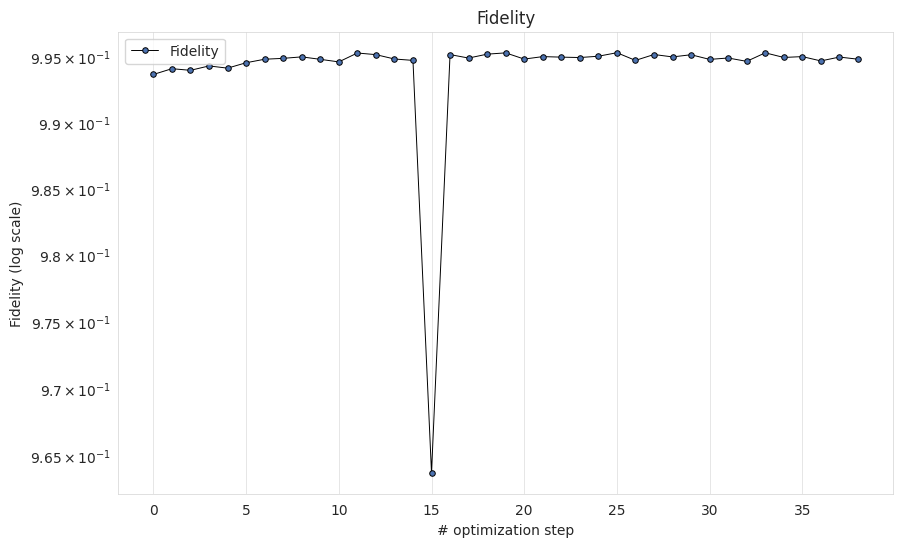
\includegraphics[width=0.45\textwidth]{figures/png/RB_optimization/NM/InitialSymplex/20241110_211211/fidelity.png}
    \caption{Plot of the average Clifford gate fidelity as a function of the optimization steps for the first round optimization - \tt{init\_symp\_1}.}
    \label{fig:20241110_211211:fidelity}
\end{figure}

\begin{figure}[h!]
    \centering
    \begin{subfigure}[t]{0.45\textwidth}
        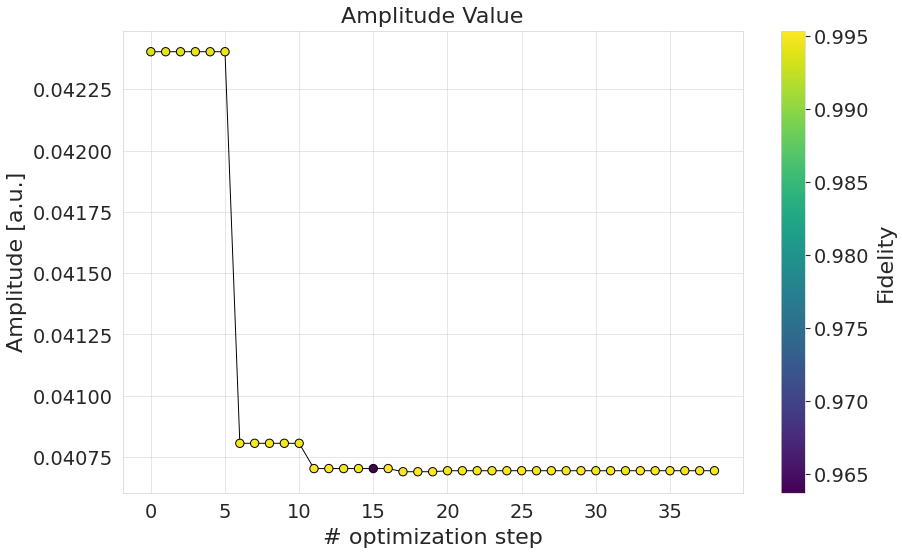
\includegraphics[width=\textwidth]{figures/png/RB_optimization/NM/InitialSymplex/20241110_211211/amplitude.png}
        \caption{Plot of the amplitude of the $R_X$ gate corresponding to different optimization steps.}
        \label{fig:20241110_211211:amplitude}
    \end{subfigure}
    \hfill
    \begin{subfigure}[t]{0.45\textwidth}
        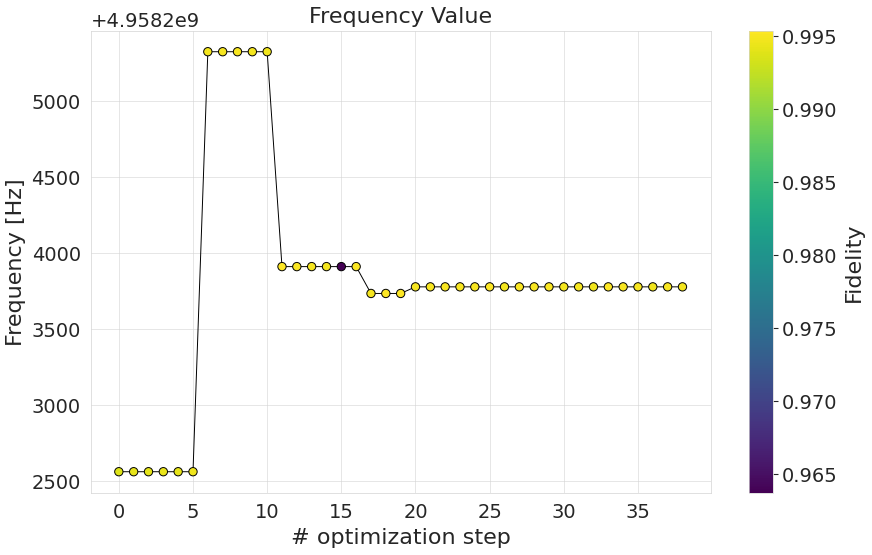
\includegraphics[width=\textwidth]{figures/png/RB_optimization/NM/InitialSymplex/20241110_211211/frequency.png}
        \caption{Plot of the frequency of the $R_X$ gate corresponding to different optimization steps.}
        \label{fig:20241110_211211:frequency}
    \end{subfigure}
    \caption{Plots of the optimization parameters as a function of the number of optimization step for the first round optimization - \tt{init\_symp\_2}.}
    \label{fig:20241110_211211:parameters}
\end{figure}

Dai plot che mostrano il risultato della prima ottimizzazione si osserva che la fidelity aumenta anche se dopo una quindicina di iterazioni si assesta attorno ad un valore di circa [inserire valore].
Due considerazioni degni di nota sono il punto relativo al sedicesimo step per cui la fidelity diminuisce notevolmente scendo sotto la soglia del 97\% (Figure \ref{fig:20241110_211211:fidelity}) nonostante ampiezza e frequenza dell'impulso $R_X$ non varino sensibilmente rispetto agli step di ottimizzazione precedenti
(see Figure \ref{fig:20241110_211211:parameters}). Il motivo di questo è da ricercarsi nel fatto che il fit per la stima della infidelity del RB fallisce (see Figure ).
Questo stesso comportamente sarà evidente anche negli altri plot che mostrano il progresso dell'ottimizzazione per questo algoritmo. 
D'altra parte una dipendenza così forte della valutazione della funzione costo dal fallimento o successo del fit dell'esponenziale della curva RB 

\begin{figure}[h!]
    \centering
    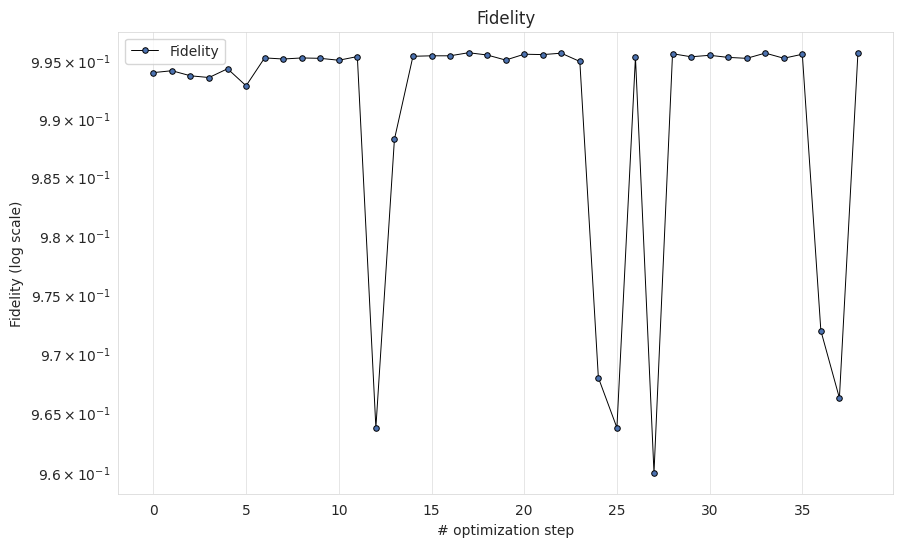
\includegraphics[width=0.45\textwidth]{figures/png/RB_optimization/NM/InitialSymplex/20241113_181711/fidelity.png}
    \caption{Plot of the average Clifford gate fidelity as a function of the optimization steps for the second round optimization - \tt{init\_symp\_2}.}
    \label{fig:20241113_181711:fidelity}
\end{figure}

\begin{figure}[ht!]
    \centering
    \begin{subfigure}[t]{0.45\textwidth}
        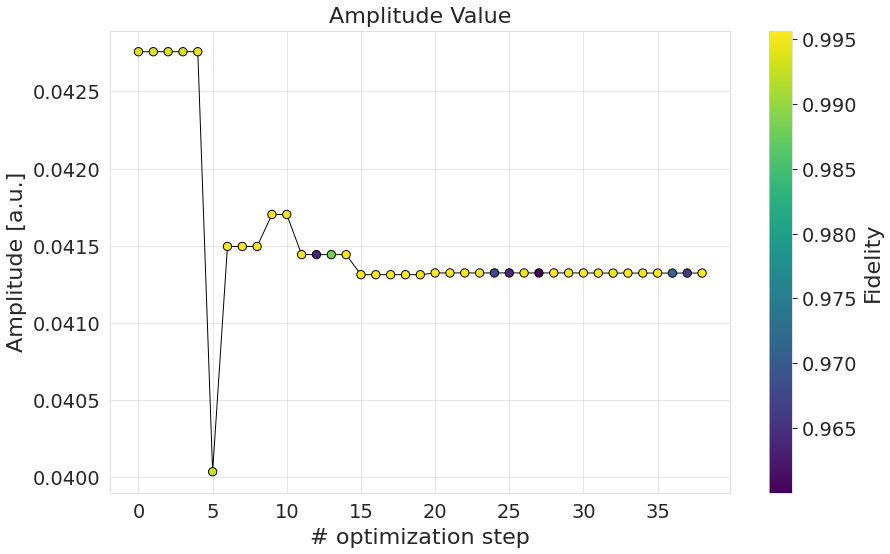
\includegraphics[width=\textwidth]{figures/png/RB_optimization/NM/InitialSymplex/20241113_181711/Amplitude.png}
        \caption{Plot of the amplitude of the $R_X$ gate corresponding to different optimization steps.}
        \label{fig:20241113_181711:amplitude}
    \end{subfigure}
    \hfill
    \begin{subfigure}[t]{0.45\textwidth}
        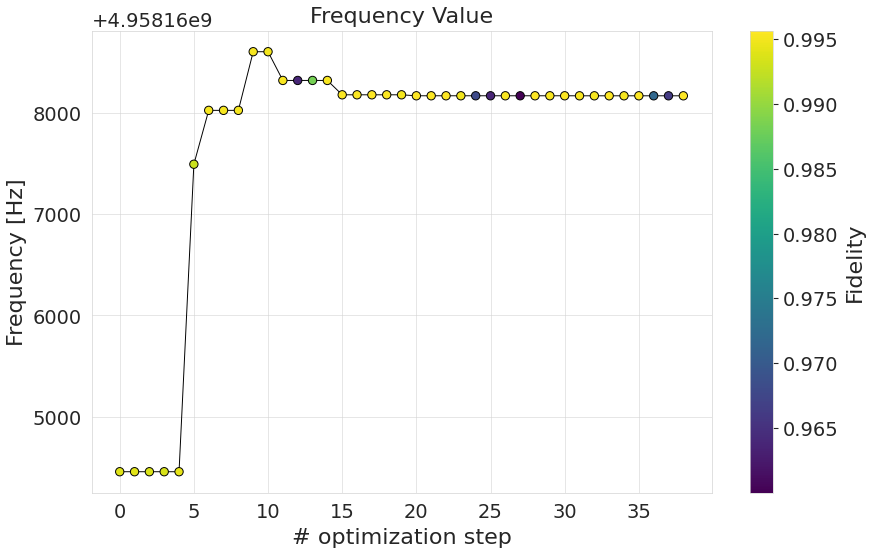
\includegraphics[width=\textwidth]{figures/png/RB_optimization/NM/InitialSymplex/20241113_181711/Frequency.png}
        \caption{Plot of the frequency of the $R_X$ gate corresponding to different optimization steps.}
        \label{fig:20241113_181711:frequency}
    \end{subfigure}
    \caption{Plots of the optimization parameters as a function of the number of optimization steps for the first round optimization - \tt{init\_symp\_2}.}
    \label{fig:20241113_181711:parameters}
\end{figure}

\begin{figure}[h!]
    \centering
    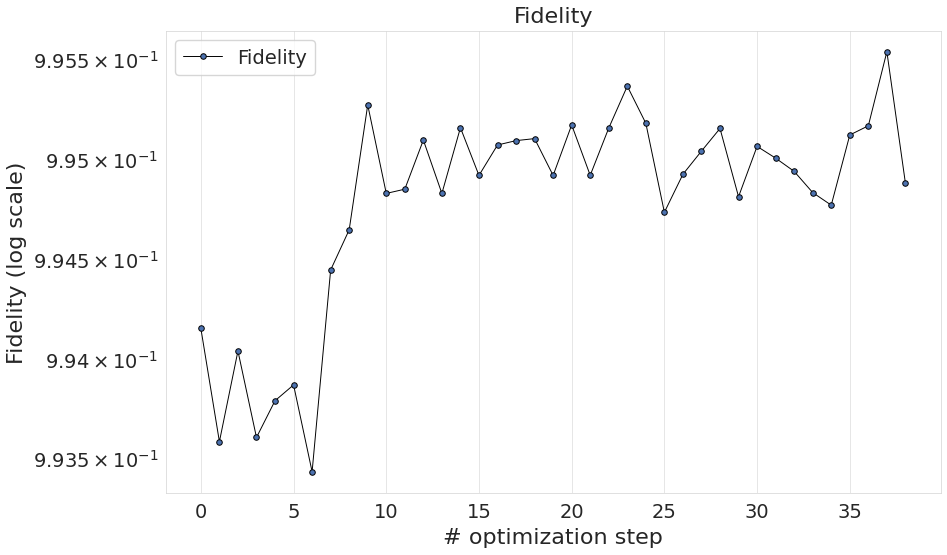
\includegraphics[width=0.45\textwidth]{figures/png/RB_optimization/NM/InitialSymplex/20241113_200745/fidelity.png}
    \caption{Plot of the average Clifford gate fidelity as a function of the optimization steps for the first round optimization - \tt{init\_symp\_3}.}
    \label{fig:20241113_200745:fidelity}
\end{figure}

\begin{figure}[ht!]
    \centering
    \begin{subfigure}[t]{0.45\textwidth}
        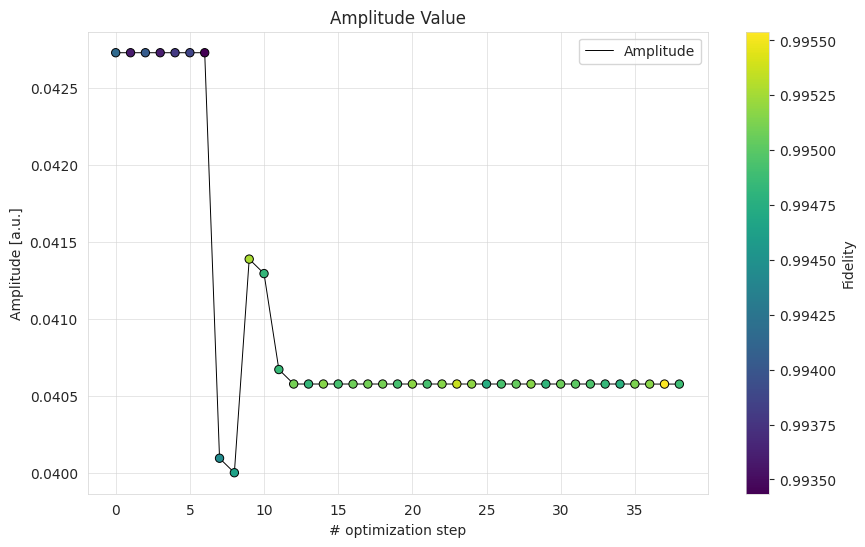
\includegraphics[width=\textwidth]{figures/png/RB_optimization/NM/InitialSymplex/20241113_200745/Amplitude.png}
        \caption{Plot of the amplitude of the $R_X$ gate corresponding to different optimization steps.}
        \label{fig:20241113_200745:amplitude}
    \end{subfigure}
    \hfill
    \begin{subfigure}[t]{0.45\textwidth}
        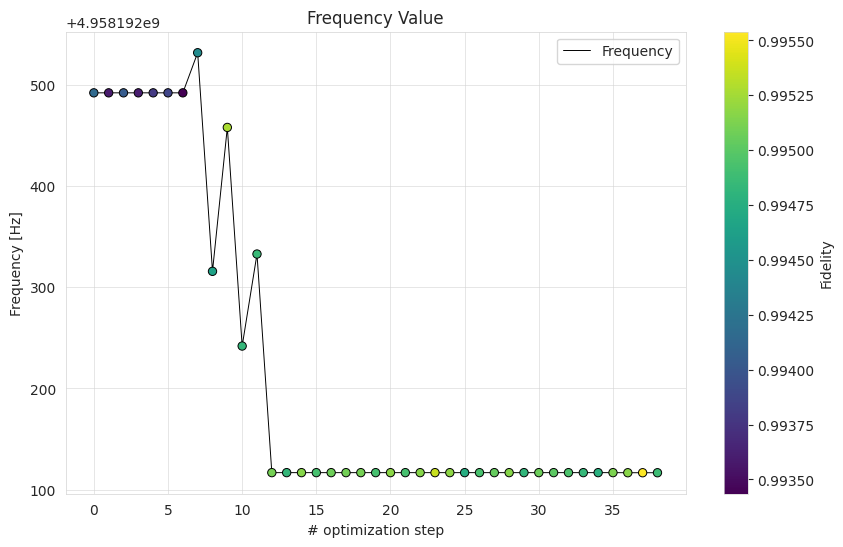
\includegraphics[width=\textwidth]{figures/png/RB_optimization/NM/InitialSymplex/20241113_200745/Frequency.png}
        \caption{Plot of the frequency of the $R_X$ gate corresponding to different optimization steps.}
        \label{fig:20241113_200745:frequency}
    \end{subfigure}
    \caption{Plots of the optimization parameters as a function of the number of optimization step for the first round optimization - \tt{init\_symp\_3}.}
    \label{fig:20241113_200745:parameters}
\end{figure}

In questo terzo e ultimo caso invece, già dal plot per la fidelity (\ref{fig:20241113_200745:fidelity}) è evidente che l'ottimizzazione non converge.

Potrebbe essere interessante confrontare i risultati per i valori dei parametri ottenuti in questi diversi tentativi di ottimizzazione, bisogna però tenere conto del fatto che, ad eccezione degli ultimi due, tutti gli esperimenti were run on different days.
Il confronto tra i valori ottenuti dall'ottimizzazione con i diversi metodi sono riportati in Figure . Dai risultati è evidente che i parametri sono soggetti a drift e che probabilmente la calibrazione ottenuta non è particolarmente stabile.

Un riassunto dei risultati ottenuti utilizzando l'algoritmo di Nelder-Mead nelle diverse configurazioni è riportato nelle prime righe di Table \ref{tab:scipy_opt}.
    
\subsection{SLSQP}
\subsubsection{Algorithm description}
Per valutare eventuali miglioramenti nella performance abbiamo provato ad utilizzare un algoritmo che fosse gradient-based. 
Nello specifico ho provato ad utilizzare l'algoritmo di Sequential Least Squares Programming (SLSQP) nella versione implementata all'interno della libreria \tt{SciPy}.

The Sequential Least Squares Programming (SLSQP) method, originally developed by Dieter Kraft in 1988 \cite{kraft1988slsqp}, is a gradient-based algorithm for solving constrained nonlinear optimization problems.
The algorithm solves a nonlinear constrained problem of the form:
\begin{align*}
& \min_{x \in \mathbb{R}^n} \quad && f(x) \\
& \text{subject to} \quad && c_i(x) = 0, \quad i = 1, \dots, m \\
& && d_j(x) \geq 0, \quad j = 1, \dots, p \\
& && \mathbf{x}^{(L)} \leq \mathbf{x} \leq \mathbf{x}^{(U)}\\
\end{align*}

It belongs to the class of Sequential Quadratic Programming (SQP) methods, which iteratively solve a sequence of quadratic programming subproblems that locally approximate the original nonlinear problem. 
\begin{enumerate}
    \item Linearization: At iteration $k$, the nonlinear constraints are approximated by their first-order Taylor expansion around the current point $\mathbf{x}_k$.
    This transforms the nonlinear constraints into a linear system locally.
    \item Quadratic subproblem construction: The objective is approximated by a quadratic model of the Lagrangian function: \begin{equation}
        \mathcal{L}(\mathbf{x}, \lambda, \mu) = f(\mathbf{x}) - \sum_{i=1}^{m} \lambda_i c_i(\mathbf{x}) - \sum_{j=1}^{p} \mu_j d_j(\mathbf{x}),
    \end{equation}
    where $\lambda_i$ and $\mu_j$ are Lagrange multipliers. 
    The Hessian of the Lagrangian is not computed explicitly, but approximated using a BFGS-like quasi-Newton update.
    \item QP Subproblem solution: A quadratic program is solved to determine a search direction $\mathbf{p}_k$, subject to the linearized constraints and bounds. 
    The subproblem minimizes the quadratic model subject to these constraints.
    \item Constrained line search: A line search is performed along $\mathbf{p}_k$ using a merit function that balances reduction in the objective with feasibility of constraints. 
    This helps ensure global convergence.
    \item Update: The iterate is updated via $\mathbf{x}_{k+1} = \mathbf{x}_k + \alpha_k \mathbf{p}_k$, where $\alpha_k$ is the step size determined by the line search. 
    The quasi-Newton approximation of the Hessian is also updated.
    \item Termination: The algorithm terminates when the norm of the projected gradient and constraint violations fall below a specified tolerance.
\end{enumerate}

If analytic derivatives for the objective or constraints are not provided, they are approximated using forward finite differences. 
In such cases, each gradient estimation requires $n+1$ function evaluations per iteration, where $n$ is the number of variables.
The values of internal parameters, such as merit function balancing terms and quasi-Newton updates, are managed internally and are not user-configurable through \tt{SciPy}.

\subsubsection{Results}
As shown in Figure \ref{fig:SLSQP:fidelity}, the optimization procedure appears to converge, a result that is also confirmed by the object returned by the \texttt{SciPy} optimizer.
This indicates that the algorithm successfully reached a local minimum within the specified tolerance of $1\cdot10^{-4}$ in less the 15 optimization steps. On the other hand, it is important to consider that SLSQP is a gradient-based method and, as such, may lack robustness in the presence of a noisy or irregular cost landscape.
This makes it susceptible to becoming trapped in local minima, especially if the optimization is not ideal.

For this run, the same constraints and parameter bounds used in the Nelder-Mead optimization were applied: a maximum of 40 optimization steps and parameter ranges setted by the initial fine-tuning routine carried out before to the fidelity optimization.

\begin{figure}[h]
    \centering
    \begin{subfigure}[t]{0.45\textwidth}
        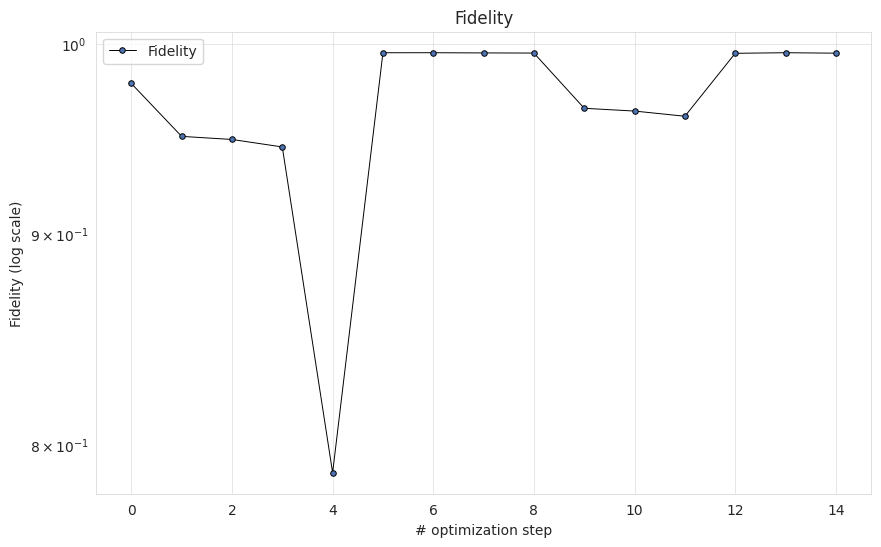
\includegraphics[width=\textwidth]{figures/png/RB_optimization/SLSQP/fidelity.png}
        \caption{Plot of the average Clifford gate fidelity as a function of the optimization steps.}
        \label{fig:SLSQP:fidelity}
    \end{subfigure}
    \hfill
    \begin{subfigure}[t]{0.45\textwidth}
        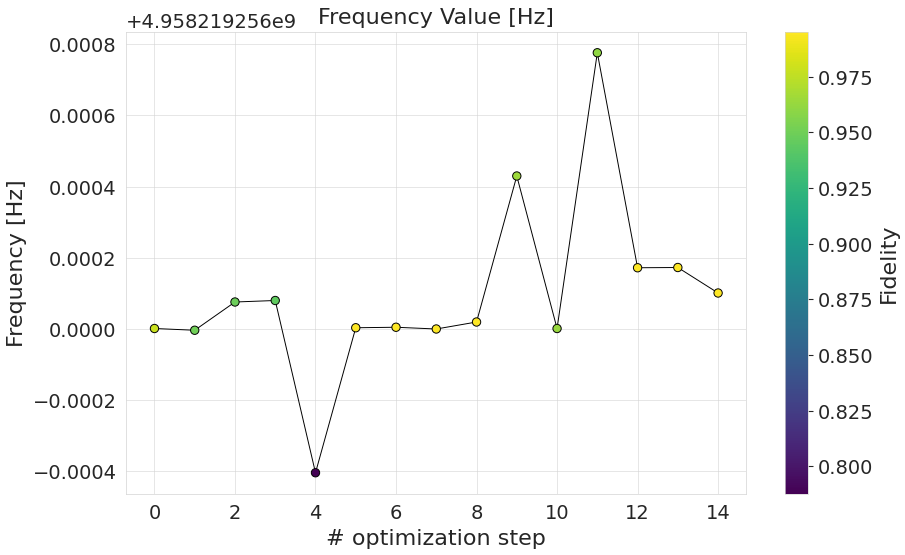
\includegraphics[width=\textwidth]{figures/png/RB_optimization/SLSQP/frequency.png}
        \caption{Plot of the frequency of the $R_X$ gate corresponding to different optimization steps.}
        \label{fig:SLSQP:frequency}
    \end{subfigure}

    \vspace{0.5cm}

    \begin{subfigure}[t]{0.45\textwidth}
        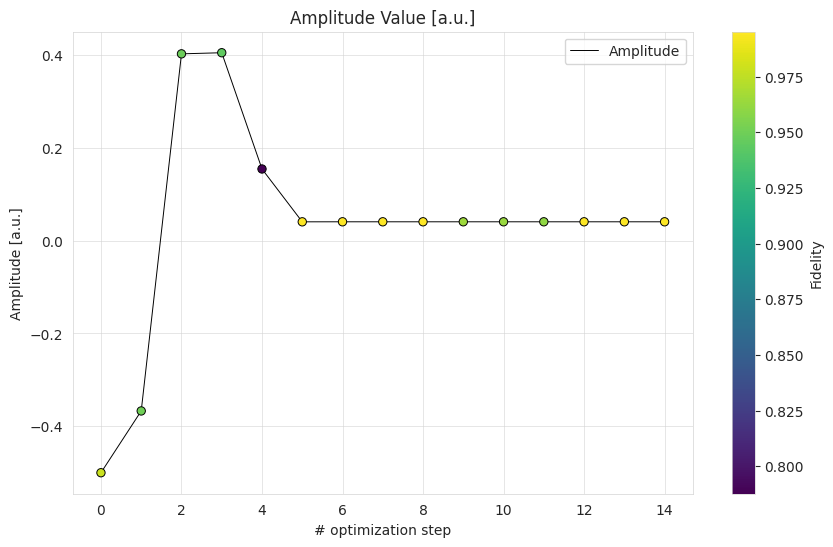
\includegraphics[width=\textwidth]{figures/png/RB_optimization/SLSQP/amplitude.png}
        \caption{Plot of the amplitude of the $R_X$ gate corresponding to different optimization steps.}
        \label{fig:SLSQP:amplitude}
    \end{subfigure}
    \hfill
    \begin{subfigure}[t]{0.45\textwidth}
        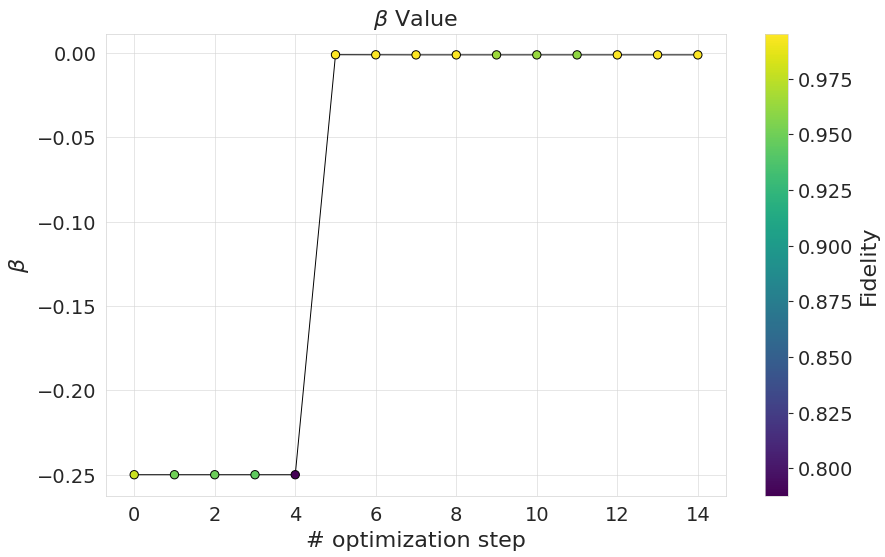
\includegraphics[width=\textwidth]{figures/png/RB_optimization/SLSQP/beta.png}
        \caption{Plot of the $\beta$ multiplying coefficient for the second quadrature component of the DRAG pulse.}
        \label{fig:SLSQP:beta}
    \end{subfigure}

    \caption{Plots of the fidelity and optimization parameters as a function of the number of optimization step for the SLSQP optimization method.}
    \label{fig:SLSQP_plots}
\end{figure}

In this case, an interesting observation is that, as expected, a sharp drop in fidelity corresponds to a frequency value that deviates significantly from the optimal one for the $R_X$ gate.
This behavior is consistent with the assumption that frequency and amplitude are the two dominant parameters in determining the quality of the $R_X$ gate and as a consequence  the average fidelity of Clifford gates.

However, as can be seen in Figure \ref{fig:SLSQP:fidelity}, the convergence behavior is not particularly stable: the fidelity exhibits large step-to-step fluctuations. 
As mentioned previously, this indicates that the SLSQP method is not robust enough to be reliably used as a systematic approach for optimizing average Clifford gate fidelity.
In particular, it becomes difficult to define a minimum number of steps beyond which a certain fidelity level can be guaranteed.

Furthermore, from a computational standpoint, this method is relatively inefficient. 
Since the gradient must be estimated numerically, each step involves multiple evaluations of the cost function, significantly increasing the total number of function calls required (see Table \ref{tab:scipy_opt}).

\begin{table}[h]
    \centering
    \begin{tabular}{lcccccc}
        \toprule
        \textbf{Method} & \textbf{Success} & \textbf{Objective Value} & \textbf{Iterations} & \textbf{RB Evaluations} & \textbf{Duration [s]}\\
        \midrule
        \textbf{Nelder-Mead} & False & 0.002732 & 40 & 93 & 2892 \\
        \textbf{init\_symplex\_1} & False &  0.004593 & 40 & 99 & 3096\\
        \textbf{init\_symplex\_2} & False & 0.004297 & 40 & 100 & 3128\\
        \textbf{init\_symplex\_3} & False & 0.004507 & 40 & 106 & 3190\\
        \textbf{SLSQP} & True & 0.004861 & 15 & 180 & 3873\\
        \bottomrule
    \end{tabular}
    \caption{This table provides a summary of the results obtained using different optimization methods available in \texttt{SciPy}.\\ 
    The \textit{Success} column indicates whether the algorithm converged successfully. 
    A value of True denotes that convergence was achieved within the specified tolerance of $1\cdot10^{-4}$ and before reaching the maximum number of iterations; otherwise, the value is False.
    The reported value of the objective function corresponds to the average Clifford gate infidelity obtained via Randomized Benchmarking (1-fidelity), which serves as the cost function minimized by the algorithm.
    The \textit{Duration} column refers to the total runtime of the script, including the initial fine-tuning stage preceding the optimization.\\}
    \label{tab:scipy_opt}
\end{table}


\section{CMA-ES}

\subsection{Algorithm description}
Covariance Matrix Adaptation Evolution Strategy (\tt{CMA-ES} \cite{cmaessimplepractical}), is a population-based evolutionary algorithm designed for optimizing complex, non-convex, and high-dimensional functions.\\
It belongs to the broader class of Evolution Strategies (ES), a subset of Evolutionary Algorithms (EAs)(see \cite{sloss20192019evolutionaryalgorithmsreview}), and is particularly effective for black-box optimization where gradient information is unavailable.

Evolution Strategies (ES) are a class of optimization methods that employ self-adaptive mechanisms to explore the search space efficiently. 
Unlike classical optimization techniques that rely on gradient descent, ES leverage stochastic sampling to navigate rugged and multimodal landscapes.
In this context, \tt{CMA-ES} is an adaptive stochastic search method that iteratively refines a probability distribution over the search space. 
Unlike traditional Genetic Algorithms (GAs), which rely on crossover and mutation operators, \tt{CMA-ES} employs a multivariate normal distribution to generate candidate solutions. 
The method adaptively updates the distribution's mean and covariance matrix based on the fitness of sampled points.

The fundamental idea behind \tt{CMA-ES} is the use of a multivariate Gaussian distribution to model promising search directions. 
Let $\mathbf{\mu}_t$ denote the mean of the distribution at iteration $t$, and $\Sigma_t$ the covariance matrix. 
Then, a new population of $\lambda$ candidate solutions $\mathbf{x}_i^{(t+1)} \sim \mathbf{\mu}_t + \sigma_t\mathcal{N}(\mathbf{\mu}_t,\mathbf{\sigma}_t^2, \Sigma_t)$, where $\sigma_t$ is a step size controlling the exploration.  

The \tt{CMA-ES} algorithm follows the following steps:\begin{enumerate}
    \item If not otherwise specified, the initial parameters are set: mean vector $\mathbf{\mu_0}$, covariance matrix $\Sigma_0$\footnote{$\Sigma_0=\mathbb{I}$ for isotropic search}, step size $\sigma_0$, population size $\lambda$
    \item Generate $\lambda$ new candidate solutions $\mathbf{x}_i$ according to a multivariate normal distribution.
    \item Evaluate the objective function $f(\mathbf{x}_i)$ for each candidate solution.
    \item Sort the new candidate solutions based on fitness: $f(\mathbf{x}_0) \leq ... \leq f(\mathbf{x}_{\lambda})$.
    \item Update the mean vector $\mathbf{\mu}$ with the $m=\lfloor \lambda / 2 \rfloor$ top performing solutions:\begin{equation}
        \mathbf{\mu} \leftarrow \sum_{i=0}^m \mathbf{w}_i\mathbf{x}_i,
    \end{equation} where $\mathbf{w}_i$ are internally defined weights.
    \item Update the isotropic and anisotropic evolution path $\mathbf{p}_{\sigma}$, $\mathbf{p}_c$ \footnote{For details on the update process of the evolution paths see \cite{cmaessimplepractical}.}.
    \item Update the covariance matrix: \begin{equation}
        C \leftarrow (1 - c_1 - c_{\mu}) C + c_1 \mathbf{p}_c \mathbf{p}_c^T + c_{\mu} \sum_{i=1}^{\mu} w_i \mathbf{y}_i \mathbf{y}_i^T,
    \end{equation} where $c_1$ and $c_\mu$ are learning rates and $\mathbf{y}_i$ represents the deviation of the $i$-th cnadidate solution from the mean $\mathbf{mu}$.
    \item Update the step size using a cumulative path evolution mechanism \begin{equation}
        \sigma \leftarrow \sigma \cdot \exp \left( \frac{c_{\sigma}}{d_{\sigma}} \left( \| \mathbf{p}_{\sigma} \| - E \| \mathcal{N}(0, I) \| \right) \right),
    \end{equation} where $c_\sigma$ is the learning rate for step-size adaptation, $d_\sigma$ is a damping factor $\| \mathbf{p}_{\sigma} \|$ is the length of the evolution path and $E \| \mathcal{N}(0, I) \|$ is the expected length of a standard normally distributed random vector.
\end{enumerate}

We decided to test \tt{CMA-ES} for the RB optimization as it is particularly well-suited for noisy or non-smooth objective functions. 
The stochastic nature of \tt{CMA-ES} allows it to remain robust against such perturbations, as it does not rely on local gradient information and instead samples across a distribution to infer promising search directions.

Unless manually specified, \tt{CMA-ES} employs internal heuristics to determine several of its hyperparameters. 
For instance, the population size $\lambda$ is typucally set according to the dimensionality of the problem:
\begin{equation}\label{eq:pop_size}
    \lambda = 4+3\lfloor \log{n}\rfloor
\end{equation}
where $n$ is the problem dimension \cite{hansen_pycma_2024}.
For full details on default parameter settings and adaptation rules, see \cite{cmaessimplepractical}.

\subsection{Results}

In the \tt{CMA-ES} optimization run, parameter settings were chosen to be as consistent as possible with those used in previous optimization algorithms.
Specifically, the initial values and the parameter bounds were defined as shown in Listing \ref{snippet:params_init}, based on the results of the preliminary fine-tuning procedure. 
The maximum number of generations was set to 30, slightly lower than the iteration limits used in the \texttt{SciPy}-based methods.
This choice was motivated by two main considerations. First, we expected a performance comparable to that of the previously tested algorithms, and that consequently 30 optimization steps (or generations) would be enough to reach an improved fidelity value.
Second we expected the algorithm to require longer execution times due to the larger number of cost functions evaluation: the population size was not manually setted but allowed to default to the internal rule od the \tt{CMA-ES} implementation, as in Equation \ref{eq:pop_size}.
In this case, with three parameters, pulse amplitude, frequency and DRAG correction parameter $\beta$, the population consisted of 7 candidate solutions per generation.
Given a population of 7 individuals and a total of 30 generations, the optimization required 210 evaluations of the objective function to complete. 

\begin{figure}[h]
    \centering
    \begin{subfigure}[t]{0.45\textwidth}
        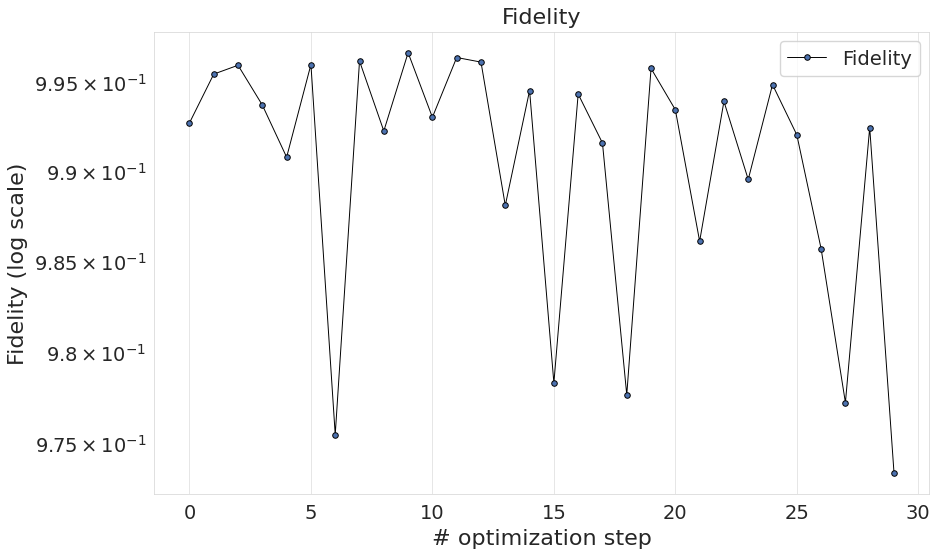
\includegraphics[width=\textwidth]{figures/png/RB_optimization/CMA/fidelity.png}
        \caption{Plot of the average Clifford gate fidelity as a function of the optimization steps.}
        \label{fig:CMA:fidelity}
    \end{subfigure}
    \hfill
    \begin{subfigure}[t]{0.45\textwidth}
        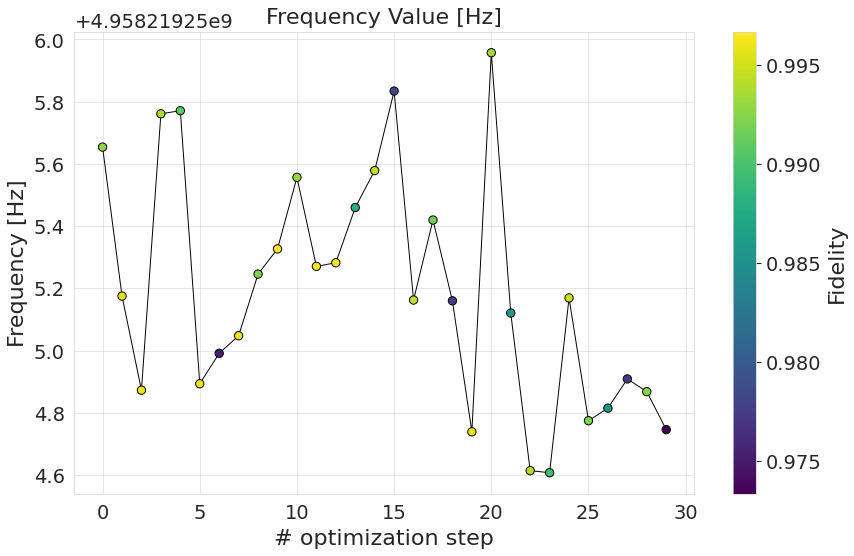
\includegraphics[width=\textwidth]{figures/png/RB_optimization/CMA/CMA_frequency.png}
        \caption{Plot of the frequency of the $R_X$ gate corresponding to different optimization steps.}
        \label{fig:CMA:frequency}
    \end{subfigure}

    \vspace{0.5cm}

    \begin{subfigure}[t]{0.45\textwidth}
        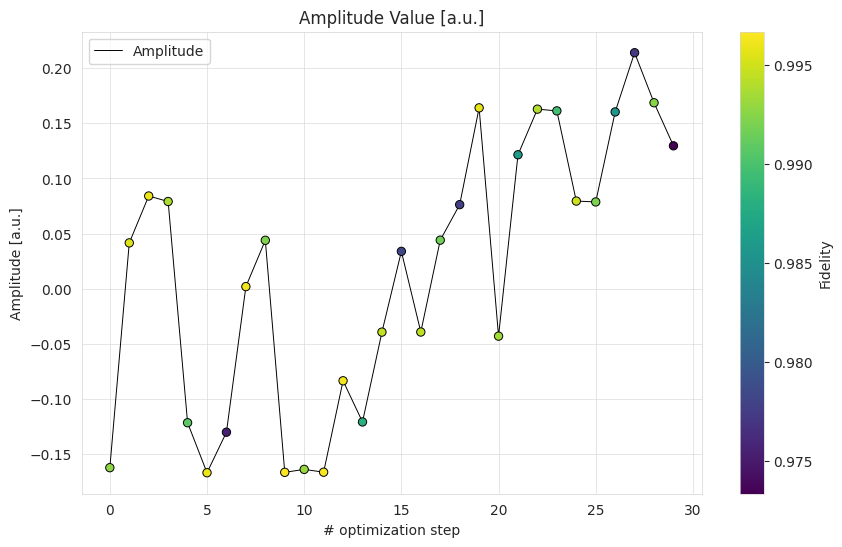
\includegraphics[width=\textwidth]{figures/png/RB_optimization/CMA/CMA_amplitude.png}
        \caption{Plot of the amplitude of the $R_X$ gate corresponding to different optimization steps.}
        \label{fig:CMA:amplitude}
    \end{subfigure}
    \hfill
    \begin{subfigure}[t]{0.45\textwidth}
        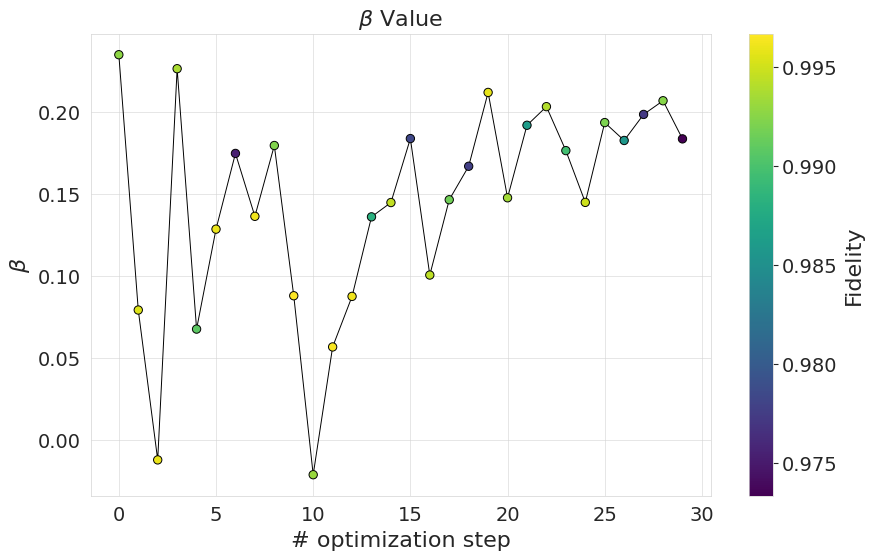
\includegraphics[width=\textwidth]{figures/png/RB_optimization/CMA/beta_CMA.png}
        \caption{Plot of the $\beta$ multiplying coefficient for the second quadrature component of the DRAG pulse.}
        \label{fig:CMA:beta}
    \end{subfigure}

    \caption{Plots of the fidelity and optimization parameters as a function of the number of optimization step for the CMA optimization method.}
    \label{fig:CMA_plots}
\end{figure}

The results of the fidelity optimization using the \tt{CMA-ES} algorithm are presented in Figure \ref{fig:CMA_plots}. 
Each point in the plots corresponds to the best-performing individual within the population at each of the 30 optimization steps (generations). 
As shown, the algorithm does not achieve full convergence within the allowed number of generations. 
This outcome is likely influenced by the relatively small population size used. 
Indeed, previous studies in the literature have demonstrated that larger populations can significantly improve the performance per function evaluation \cite{hansen2004evaluating}, obviously at the cost of increased computational time.

The choice to limit both the number of generations and the population size was made deliberately to maintain a manageable total runtime. 
Increasing either of these parameters would have led to a substantial rise in computational cost, as \tt{CMA-ES} evaluates the objective function $\lambda$ times per generation where $\lambda$ is the population size.

Another factor that negatively influenced the algorithm convergence is the choice of the initial step size parameter, $\sigma = 0.25$. 
In \tt{CMA-ES} $\sigma$ controls the standard deviation of the multivariate normal distribution used to generate the first population, thereby determining how broadly the algorithm explores the parameter space around the initial guess. 
A smaller $\sigma$ would have concentrated the search in a narrower region, possibly leading to faster convergence to a local optimum. 
However, this value of $\sigma = 0.25$ was chosen with the goal to explore a wider portion of the parameter space than in previous \texttt{SciPy}-based optimizations, in order to investigate the possible presence of higher-fidelity regions that had not yet been sampled.

\section{Optuna}

\subsection{Algorithm description}

The Tree-Structured Parzen Estimator (TPE) algorithm, as implemented in the \tt{Optuna} optimization framework \cite{optuna_2019}, is a model-based, derivative-free optimization method. 
\tt{Optuna} belongs to the class of Sequential Model-Based Optimization (SMBO) strategies \cite{SMBO_proceedings}, which iteratively refine a surrogate model of the objective function based on past evaluations and select new points in parameter space by balancing exploration and exploitation \cite{BayesianOptimizationReview}.

The TPE method differs from classical Gaussian Process-based Bayesian optimization by using non-parametric density estimation to guide the search through parameter space. 
Instead of directly modeling the objective function $f(\mathbf{x})$, TPE models the conditional probability distribution of the parameters $\mathbf{x}$ given the value of the objective function.

Given a set of past observations $\{ (\mathbf{x}_i, y_i) \}_{i=1}^N$, where $ y_i = f(\mathbf{x}_i) $, the algorithm proceeds as follows:

\begin{enumerate}
    \item Split the observations: Define a threshold value $ y^* $, typically chosen as a quantile of the observed objective values. 
        The dataset is then split into two subsets:
        \begin{itemize}
            \item $\mathcal{L} = \{ \mathbf{x}_i : y_i < y^* \}$, the set of promising configurations
            \item $\mathcal{G} = \{ \mathbf{x}_i : y_i \geq y^* \}$, the set of less promising configurations
        \end{itemize}
    \item Estimate densities: Construct two kernel density estimators (KDEs) to approximate the conditional densities:
    \[
    l(\mathbf{x}) \approx p(\mathbf{x} \mid y < y^*) \quad \text{and} \quad g(\mathbf{x}) \approx p(\mathbf{x} \mid y \geq y^*).
    \]
    \item Candidate sampling: Draw a number of candidate parameter configurations $\mathbf{x}$ from the distribution $l(\mathbf{x})$, which is biased toward more promising regions of the search space.
    \item Acquisition function: For each sampled candidate $\mathbf{x}$, compute the ratio
    \[
    \text{EI}(\mathbf{x}) = \frac{l(\mathbf{x})}{g(\mathbf{x})},
    \]
    which serves as an acquisition function analogous to expected improvement. The candidate with the highest ratio is selected for evaluation.
    \item Evaluate and update: Evaluate the objective function $ y = f(\mathbf{x}) $ at the selected configuration and append the result to the history. Return to step 1.
\end{enumerate}
This process continues until a stopping criterion is met, such as a maximum number of trials or convergence of the best observed value.

Differently from other TPE implementations, \tt{Optuna} supports automatic pruning designed to terminate unpromising trials early, thus reducing computational cost. 
In common applications such as neural network training, pruning is enabled by reporting intermediate objective values via \texttt{trial.report(...)} and comparing them to statistics of previously completed trials. 
By default, \texttt{Optuna} employs the \texttt{MedianPruner}, which terminates a trial if its intermediate value is worse than the median of completed trials at the same step.

In the present work, the cost function is defined as the infidelity extracted from a complete randomized benchmarking (RB) routine and the optimization problem involves a low-dimensional parameter space, comprising only three continuous parameters; given these characteristics pruning was not applied.

\subsection{Results}

\subsection{$\beta$ parameter impact on RB optimization}

\paragraph{D1 - 30 steps}

\paragraph{D1 - 100 steps}

\paragraph{D1 - 1000 steps}

\paragraph{D1 - 1000 steps}



\section{RB optimization conclusions}
As mentioned in the introduction to this chapter, the primary objective of this work was to evaluate whether it is possible to develop an automated optimization routine that can be executed directly on quantum hardware to periodically improve the fidelity of single-qubit gates—specifically the  $R_X(\pi)$ gate. 
For such a routine to be practically useful, two main conditions must be met: first, the optimization must lead to a consistent and measurable improvement in gate fidelity within a limited amount of time; 
second, the routine must demonstrate stable convergence, such that the resulting optimized parameters (amplitude, frequency, and DRAG correction) can reliably be used to update the hardware configuration, ensuring a reproducible improvement in performance.

While the protocol did yield fidelity improvements in several cases, the results indicate that the implementation we built to be run on hardware is not yet robust or efficient enough for routine use. 
The main limiting factor is the duration of the Randomized Benchmarking routine used to evaluate gate fidelity, which is relatively long. 
Because the optimization procedure requires several evaluations of this cost function, the total execution time quickly becomes a bottleneck. 
Furthermore, we observed that convergence is not always guaranteed: in some cases, the optimization either stalls or does not lead to meaningful improvements within the time frame or number of iterations considered acceptable for practical deployment.

In summary, although the tests suggests that automated gate fidelity optimization is in principle possible, the current implementation does not meet the reliability and efficiency requirements needed for scheduled, hardware-level recalibration. 
Improvements could focus on accelerating cost function evaluation or designing more robust optimization strategies with stronger convergence guarantees.

Due possibili estensioni degli studi e dei risultati che sono stati presentati in questo capitolo, entrambi interessanti possono essere innanzitutto un tentativo di ottimizzazione dei parametri del RB per rendere più efficiente la procedura.
In questo caso sono stati utilizzati circuiti con una profondità di 1000 e per ogni profondità da valutare sono state campionati 1000 diversi circuiti.
Considerando il costo computazionale della valutazione dell'RB sicuramente potrebbe essere utile cercare di rendere questa ottimizzazione più efficiente riducendo la profondità del circuiuto o il numero di circuiti fenerati, in questo senso potrebbe essere utile fare uno studio più dettagliato sia sul piano teorico che sul piano computazionale (tipo hyperparameter optimization) per studiare 
i valori migliori per questi parametri. È probabile che entrambi questi valori possano essere ridotti rendendo quindi l'ottimizzazione più efficiente e potenzialmente feasable e utilizzabile per migliorare la avarage Clifford gate fidelity in maniera automatica sul chip e quindi renderla una routine utilizzabile prima di girare circuiti o algoritmi quantistici.

L'altro studio che potrebbe essere effettuato partendo da questi risultati riguarda l'ottimizzazione dei parametri con cui sono stati runnati gli algoritmi di ottimizzazione, nel caso di CMA ad esempio è evidente che l'algoritmo non converge ma ad esempio si può studiare l'impatto dell'aumento della popolazione in ciascuna generazione (che però ha l'inevitabile trade-off di aumentare il costo computazionale dell'ottimizzazione) o della riduzione della sigma nella generazione della popolazione stessa.
Questa seconda operazione in particolare indubbiamente migliorerebbe la convergenza dell'algoritmo riducendone tuttavia l'esplorazione di altre configurazioni di parametri.
Entrambi questi studi potrebbero essere particolarmente interessanti soprattutto in un contesto in cui però la calibrazione si mostra più stabile (inserire riferimento al confronto + distanza percentuale tra i valori dei parametri).

In questo caso abbiamo scelto di non procedere in questa direzione soprattutto per via dei risultati che sono stati ottenuti con \tt{optuna}, gli ultimi studi in particolare con un numero elevato di trials hanno messo in luce quanto, nonostane una buona esplorazione dello spazio dei parametri non sia facile ottenere una configurazione con una buuona fidelity sufficientemente stabile. 

\begin{sidewaystable}[h]
    \centering
    \begin{tabular}{lccccccccccc}
        \toprule
        \textbf{Analysis} & \textbf{Initial} & \textbf{Best} & \textbf{Best} & \textbf{Amplitude} & \textbf{Frequency} & \textbf{$\beta$} & \textbf{Best cost} & \textbf{Initial} & \textbf{Best} & \textbf{Best fidelity} \\
        \textbf{Name} & \textbf{cost} & \textbf{cost} & \textbf{index} & \textbf{best [a.u.]} & \textbf{ best [$\times10^9$ Hz]} & \textbf{best} & \textbf{improv. [\%]} & \textbf{fidelity} & \textbf{fidelity} & \textbf{improv[\%]} \\
        \midrule
        \textbf{Nelder\_Mead} & 0.00983 & 0.00269 & 19 & 0.04063 & 4.95701 & -1.53253 & 72.59 & 0.99017 & 0.99731 & 0.72 \\
        \textbf{init\_simplex\_1} & 0.00633 & 0.00467 & 25 & 0.04069 & 4.95820 &  & 26.23 & 0.99367 & 0.99533 & 0.17 \\
        \textbf{init\_simplex\_2} & 0.00607 & 0.00436 & 17 & 0.04131 & 4.95817 &  & 28.27 & 0.99393 & 0.99564 & 0.17 \\
        \textbf{init\_simplex\_3} & 0.00585 & 0.00446 & 37 & 0.04058 & 4.95819 &  & 23.73 & 0.99415 & 0.99554 & 0.14 \\
        \textbf{SLSQP} & 0.02172 & 0.00482 & 13 & 0.04058 & 4.95822 & -0.00115 & 77.79 & 0.97828 & 0.99518 & 1.73 \\
        \textbf{CMA-ES} & 0.00728 & 0.00335 & 9 & -0.16634 & 4.95822 & 0.08802 & 54.04 & 0.99272 & 0.99665 & 0.40 \\
        \textbf{optuna\_30} & & & & & & & & & & \\
        \textbf{optuna\_100} & & & & & & & & & & \\
        \textbf{optuna\_1000} & & & & & & & & & & \\
        \textbf{optuna} & & & & & & & & & & \\
        \bottomrule
    \end{tabular}
    \caption{Comparison of Initial and Best Values}
    \label{tab:best_values}
\end{sidewaystable}

\begin{sidewaystable}[h]
    \centering
    \begin{tabular}{lcccccccccc}
        \toprule
        \textbf{Analysis} & \textbf{Initial} & \textbf{Final} & \textbf{Amplitude} & \textbf{Frequency} & \textbf{$\beta$} & \textbf{Final cost} & \textbf{Initial} & \textbf{Final} & \textbf{Final fidelity} \\
        \textbf{Name} & \textbf{cost} & \textbf{cost} & \textbf{final [a.u.]} & \textbf{final [$\times10^9$ Hz]} & \textbf{final} & \textbf{improv. [\%]} & \textbf{fidelity} & \textbf{fidelity} & \textbf{improv. [\%]} \\
        \midrule
        \textbf{Nelder\_Mead} & 0.00983 & 0.00295 & 0.04067 & 4.95699 & -1.53976 & 70.02 & 0.99017 & 0.99705 & 0.69 \\
        \textbf{init\_simplex\_1} & 0.00633 & 0.00517 & 0.04069 & 4.95820 &  & 18.41 & 0.99367 & 0.99483 & 0.12 \\
        \textbf{init\_simplex\_2} & 0.00607 & 0.00437 & 0.04132 & 4.95817 &  & 28.10 & 0.99393 & 0.99563 & 0.17 \\
        \textbf{init\_simplex\_3} & 0.00585 & 0.00512 & 0.04058 & 4.95819 &  & 12.46 & 0.99415 & 0.99488 & 0.07 \\
        \textbf{SLSQP} & 0.02172 & 0.00507 & 0.04058 & 4.95822 & -0.00115 & 76.64 & 0.97828 & 0.99493 & 1.70 \\
        \textbf{CMA-ES} & 0.00728 & 0.02664 & 0.12956 & 4.95822 & 0.18364 & -265.93 & 0.99272 & 0.97336 & -1.95 \\
        \textbf{optuna\_30} & & & & & & & & & \\
        \textbf{optuna\_100} & & & & & & & & & \\
        \textbf{optuna\_1000} & & & & & & & & & \\
        \textbf{optuna} & & & & & & & & & \\
        \bottomrule
    \end{tabular}
    \caption{}
    \label{tab:final_values}
\end{sidewaystable}

\begin{comment}
    \begin{sidewaystable}[h]
    \centering
    \begin{tabular}{lcccccccccccccccccc}
        \toprule
        \textbf{Analysis} & \textbf{Initial} & \textbf{Best} & \textbf{Best} & \textbf{Amplitude} & \textbf{Frequency} & \textbf{$\beta$} & \textbf{Cost} & \textbf{Amplitude} & \textbf{Frequency} & \textbf{$\beta$} & \textbf{Best cost} & \textbf{Final cost} & \textbf{Initial} & \textbf{Best} & \textbf{Final} & \textbf{Best fidelity} & \textbf{Final fidelity} \\
        \textbf{Name} & \textbf{cost} & \textbf{cost} & \textbf{index} & \textbf{best [a.u.]} & \textbf{best [$\times10^9$ Hz]} & \textbf{best} & \textbf{final} & \textbf{final [a.u.]} & \textbf{final [$\times10^9$ Hz]} & \textbf{final} & \textbf{improv. [\%]} & \textbf{improv. [\%]} & \textbf{fidelity} & \textbf{fidelity} & \textbf{fidelity} & \textbf{improv. [\%]} & \textbf{improv. [\%]} \\
        \midrule
        \textbf{Nelder\_Mead} & 0.00983 & 0.00269 & 19 & 0.04063 & 4.95701 & -1.53253 & 0.00295 & 0.04067 & 4.95699 & -1.53976 & 72.59 & 70.02 & 0.99017 & 0.99731 & 0.99705 & 0.72 & 0.69 \\
        \textbf{init\_simplex\_1} & 0.00633 & 0.00467 & 25 & 0.04069 & 4.95820 &  & 0.00517 & 0.04069 & 4.95820 &  & 26.23 & 18.41 & 0.99367 & 0.99533 & 0.99483 & 0.17 & 0.12 \\
        \textbf{init\_simplex\_2} & 0.00607 & 0.00436 & 17 & 0.04131 & 4.95817 &  & 0.00437 & 0.04132 & 4.95817 &  & 28.27 & 28.10 & 0.99393 & 0.99564 & 0.99563 & 0.17 & 0.17 \\
        \textbf{init\_simplex\_3} & 0.00585 & 0.00446 & 37 & 0.04058 & 4.95819 &  & 0.00512 & 0.04058 & 4.95819 &  & 23.73 & 12.46 & 0.99415 & 0.99554 & 0.99488 & 0.14 & 0.07 \\
        \textbf{SLSQP} & 0.02172 & 0.00482 & 13 & 0.04058 & 4.95822 & -0.00115 & 0.00507 & 0.04058 & 4.95822 & -0.00115 & 77.79 & 76.64 & 0.97828 & 0.99518 & 0.99493 & 1.73 & 1.70 \\
        \textbf{CMA-ES} & 0.00728 & 0.00335 & 9 & -0.16634 & 4.95822 & 0.08802 & 0.02664 & 0.12956 & 4.95822 & 0.18364 & 54.04 & -265.93 & 0.99272 & 0.99665 & 0.97336 & 0.40 & -1.95 \\
        \textbf{optuna\_30} & & & & & & & & & & & & & & & & & \\
        \textbf{optuna\_100} & & & & & & & & & & & & & & & & & \\
        \textbf{optuna\_1000} & & & & & & & & & & & & & & & & & \\
        \textbf{optuna} & & & & & & & & & & & & & & & & & \\
        \bottomrule
    \end{tabular}
    \caption{}
    \label{tab:detailed_results}
\end{sidewaystable}

\begin{table}[h]
    \centering
    \begin{tabular}{lccc}
        \textbf{Analysis Name} & \textbf{# function evaluations} & \textbf{# optimization steps} & \textbf{time [s]}
        \hline
        \textbf{D1\_nelder-mead\_post\_ft\_true} & 93 & 39 & 2892 \\
        \textbf{D1_SLSQP} & 180 & 15 & 3873 \\
        \textbf{D1\_cma\_post\_ft\_true} & 210 & 30 & 4836 \\
        \textbf{D1\_init\_simplex\_20241110\_211211} & 99 & 39 & 3096 \\
        \textbf{D1\_init\_simplex\_20241113\_181711} & 100 & 39 & 3128 \\
        \textbf{D1\_init\_simplex\_20241113\_200745} & 106 & 39 & 3190 \\
        \textbf{}
    \bottomrule
    \end{tabular}
    \caption{}
    \label{tab:cal_results}
\end{table}
\end{comment}
\chapter{Pulses analysis and tuning}

Having concluded that closed-loop optimization would not significantly improve fidelity, we shifted our focus towards improvement and implementation of individual protocols to improve the accuracy of qubit operations.\\
In this chapter, I present the results of two additions to the \texttt{Qibocal} software. 
The first is the inclusion of an $RX90$ gate as a native gate, which can enhance the performance of protocols requiring qubit rotations of $\frac{\pi}{2}$.
The second is the implementation of the cryoscope, a routine first described in \cite{rol_time-domain_2020}, which is useful for correcting distortions in the magnetic flux pulse applied to the SQUID.

\section{RX90 calibration}



\section{Flux pulse correction}
\subsection{Notes on signal analysis}


\subsection{Cryoscope}
The experiment that we describe in this section was first introduced in \cite{rol_time-domain_2020}, the goal is to determine predistortions that needs to be applied to a flux pulse signal so that the qubit receives the flux pulse as intended by the experimenter.

As explained in section \ref{sec:cQED}, accurate dynamical control of qubit frequency is of key importance to realize single- and two-qubit gates.
One of the on-chip control variable that is used on QunatumWare chip is the magnteic flux through a SQUID loop, the signal for magnetic flux control originates from an arbitrary waveform genarator (AWG) which operates at room temperature.\\
As the signal propagates through various electrical components along the control line leading to the quantum device it undergoes linear dynamical distortions. 
If not properly compensated, these distortions can degrade gate performance, impacting experiments fidelity and repeatability.\\

In \cite{rol_time-domain_2020} is proposed a technique to characterize flux-pulse distortions induced by components inside the dilution refrigerator by directly measuring the qubit state.
In this protocol we send the qubit a pulse sequence where a flux pulse of varying duration $\tau$ is embedded between two $\frac{\pi}{2}$ pulses which are always separated by a fixed interval $T_{sep}$.\\
The first $\frac{\pi}{2}$ pulse rotates the qubit of $\frac{\pi}{2}$ around the $y$ axis of the Bloch sphere changing its state from $\ket{0}$ to $\frac{\ket{0}+\ket{1}}{\sqrt{2}}$.

When a flux pulse $\Phi_{Q,\tau}(t)$ of duration $\tau$ is sent to the qubit\footnote{To send a $\Phi_{Q,\tau}(t)$ flux pulse we are actually sending a $V_{\text{in},\tau}(t)$ voltage pulse through the electronics} after the first $\frac{\pi}{2}$ pulse, the qubits evolve to the state $\frac{\ket{0}+e^{i\varphi_\tau}\ket{1}}{\sqrt{2}}$ with relative quantum phase 
\begin{equation}\label{eq:phi}
    \frac{\varphi_{\tau}}{2\pi} = \int_{0}^{T_{sep}} \Delta f_Q (\Phi_{Q,\tau(t)})\text{d}t = \int_{0}^{\tau} \Delta f_Q (\Phi_{Q,\tau(t)})\text{d}t + \int_{\tau}^{T_{sep}} \Delta f_Q (\Phi_{Q,\tau(t)})\text{d}t
\end{equation}
where in the second step we separated the contributions from flux response up to $\tau$ and the turn-off transient. 

The experiment is then completed with a $\frac{\pi}{2}$ rotation aroud the $y$- or $x$-axis of the Bloch sphere to measure respectively the $\langle X \rangle$ or $\langle Y \rangle$ components of the Bloch vector when applying the measurement gate $MZ$. 
From the measurement of $\langle X \rangle$ and $\langle Y \rangle$ we can extract the relative phase $\phi_{\tau}$.\\

Then we can estimate $\Phi_Q(t)$ in the interval $[\tau,\tau+\Delta\tau]$ as follows. From the measurement of $\phi_{\tau + \Delta\tau}$ and $\phi_\tau$ we can compute $\overline{\Delta f_R}$:
\begin{align}\label{eq:detuning}
    \overline{\Delta f_R} &= \frac{\phi_{\tau+\Delta\tau} - \phi_\tau}{2\pi\Delta\tau}\\ 
    &= \frac{1}{\Delta\tau}\left(\int_{0}^{\tau+\Delta\tau}\Delta f_Q (\Phi_{Q,\tau+\Delta\tau}(t))dt + \int_{\tau+\Delta\tau}^{T_{sep}}\Delta f_Q (\Phi_{Q,\tau+\Delta\tau}(t))dt\right) \\
    &-\frac{1}{\Delta\tau}\left(\int_{0}^{\tau}\Delta f_Q (\Phi_{Q,\tau}(t))dt - \int_{\tau}^{T_{sep}}\Delta f_Q (\Phi_{Q,\tau}(t))dt\right)\\
    &=\frac{1}{\Delta\tau}\left(\int_{\tau}^{\tau+\Delta\tau} \Delta f_Q(\Phi_{Q,\tau+\Delta\tau})dt + \int_{\tau+\Delta\tau}^{T_{sep}}\Delta f_Q (\Phi_{Q,\tau+\Delta\tau}(t))dt - \int_{\tau}^{T_{sep}}\Delta f_Q (\Phi_{Q,\tau}(t))dt\right)\\
    &= \frac{1}{\Delta\tau}\int_{\tau}^{\tau+\Delta\tau} \Delta f_Q(\Phi_{Q,\tau+\Delta\tau})dt + \varepsilon
\end{align}  
with \[\varepsilon = \frac{1}{\Delta\tau}\left(\int_{\tau+\Delta\tau}^{T_{sep}}\Delta f_Q (\Phi_{Q,\tau+\Delta\tau}(t))dt - \int_{\tau}^{T_{sep}}\Delta f_Q (\Phi_{Q,\tau}(t))dt\right)\]
The phase contribution from the turn-off transients is minimal due to the sharp return to the first-order flux-insensitive sweet spot of the nearly quadratic $\Delta f_Q(\Phi_Q)$; 
numerical simulations suggest that $|\varepsilon|/\Delta f_R$ remains within the range of approximately $10^{-2}$ to $10^{-3}$ for typical dynamical distortions in commonly used electronic components\cite{negligible}\cite{Langford2017}, for this reason it will be neglected.\\

Then we can obtain the reconstructed flux pulse $\Phi_R(t)$ inverting eq. \ref{eq:freqdepndenceonflux}.
\subsubsection{Pulse reconstruction}

\subsubsection{Corrections study}

\subsection{Corrected pulse}

\begin{comment}
    TO DO LIST:
    * calcoli analitici di convoluzioni per dimostrare che è giusto il modo in cui combiniamo i filtri
    * eventualmente provare ad aggiungere più correzioni esponenziali
\end{comment}
\subsection{Filter determination}
\subsubsection{IIR}
\subsubsection{FIR}
for description and notes on \tt{CMA-ES} see section \ref{Sec:OptimizationMethods}
\subsubsection{Output filters in QM}

\subsection{dimostrazione del conto}

In general, for different forms of the detuning flux $\Delta f(\Phi) = a\Phi^k$, where $k \in \mathbb{Z}^+$, the phase $\varphi_\tau$ expressed in terms of the impulse response $h =\frac{\text{d}s}{\text{d}t}$ is the following,
\begin{equation}\label{eq:demonstarted}
    \varphi_\tau = 2\pi a \int_{0}^{\infty} \left[ \int_{0}^{\infty} h(t - t') dt' - \int_{0}^{\infty} h(t - \tau - t') dt' \right]^k dt = 2\pi a \int_{0}^{\tau} \left[ \int_{0}^{t} h(t - t') dt' \right]^k dt + 2\pi a \int_{\tau}^{\infty} \left[ \int_{0}^{\tau} h(t - t') dt' \right]^k dt,
\end{equation}

The demonstration of this equality is reported in Appendix C \ref{app:AppendixC}.

\begin{equation}
    
\end{equation}

%conclusion and outlook
\chapter{Conclusions and outlook}



% APPENDICES
\appendix
\cleardoublepage
\chapter*{Appendix A} 
\label{app:AppendixA}




\chapter*{Appendix B}
\label{app:AppendixB}

In the following we will demonstrate the corrctness of equation \ref{eq:demonstarted}:

\begin{align}
    \varphi_\tau &= 2\pi a \int_{0}^{\infty} \left[ \int_{0}^{\infty} h(t - t') dt' - \int_{0}^{\infty} h(t - \tau - t') dt' \right]^k dt \\
    &= 2\pi a \int_{0}^{\tau} \left[ \int_{0}^{t} h(t - t') dt' \right]^k dt + 2\pi a \int_{\tau}^{\infty} \left[ \int_{0}^{\tau} h(t - t') dt' \right]^k dt,
\end{align}
for different forms of the detuning flux 
\begin{equation}\label{eq:det_flux}
    \Delta f(\Phi) = a\Phi^k
\end{equation}
where $k \in \mathbb{Z}^+$.
From the calculations showed in \ref{eq:phi} we know that the relative phase $\phi_\tau$ for a general form of the detuning flux \ref{eq:det_flux}, with $T_{\text{sep}} = \infty$ is
\begin{equation}\label{eq:phi_here}
    \varphi_{\tau} = 2\pi \int_{0}^{+\infty} a \left[ \left( s(t) - s(t - \tau) \right) \right]^k dt = 2\pi a \int_{0}^{+\infty} \left[ \left( s(t) - s(t - \tau) \right) \right]^k dt
\end{equation}

As hypothesis we know that voltage-to-flux step response of the control line is 
\begin{equation}\label{eq:voltage_to_flux}
    s(t) = \left(1 - e^{-t/\tau} \right) \cdot u(t),
\end{equation} where $u(t)$ is the step function, and that the impulse response is 
\begin{equation}\label{eq:h_def}
    h(t) = \frac{\text{d}s}{\text{d}t}
\end{equation}


If we substitute the expression of $s(t)$ given in \ref{eq:voltage_to_flux} in equation \ref{eq:phi_here} we obtain
\begin{equation}\label{eq:first_step_dem}
    \varphi_{\tau} = 2\pi a \int_{0}^{+\infty} \left[ \int_{0}^{+\infty} h(t - t') dt' - \int_{0}^{+\infty} h(t - \tau - t') dt' \right]^k dt.
\end{equation}

To do we have to show that \begin{enumerate}
    \item \begin{equation}\label{eq:first_dem}
        s(t) = \int_0^{+\infty} h(t-t')dt'
    \end{equation}
    \item \begin{equation}\label{eq:sec_dem}
        s(t-\tau) = \int_{0}^{+\infty} h(t-\tau-t')dt'
    \end{equation}
\end{enumerate}

We start from the demonstration of equation \ref{eq:first_dem}. By definition \ref{eq:h_def} we can write
\begin{equation}\label{eq:first_dem1}
    h(t) = \frac{d}{dt} \left[ \left(1 - e^{-t/\tau} \right) u(t) \right] = \frac{e^{-t/\tau}}{\tau} u(t) + \left(1 - e^{-t/\tau} \right) \delta(t), 
\end{equation}

substituting Eq \ref{eq:first_dem1} in Eq \ref{eq:first_dem} we obtain \begin{equation}
    \int_{0}^{+\infty} h(t - t') dt' = \int_{0}^{+\infty} \frac{e^{-\frac{(t - t')}{\tau}}}{\tau} u(t - t') dt' + \int_{0}^{+\infty} \left(1 - e^{-(t - t')/\tau} \right) \delta(t - t') dt',
\end{equation}
by setting $t'' = t-t'$, $dt''=-dt'$,  we have $t''\rightarrow -\infty$ for $t'\rightarrow +\infty$ and $t''= t$ for $t'= 0$, the integral then becomes
\begin{align}
    \int_{0}^{+\infty} h(t - t') dt' &= \int_{t}^{-\infty} -\frac{e^{-t''/\tau}}{\tau} u(t'') dt'' - \int_{t}^{-\infty} \left(1 - e^{-t''/\tau} \right) \delta(t'') dt'' \\
    &= \int_{-\infty}^{t} \frac{e^{-t''/\tau}}{\tau} u(t'') dt'' + \int_{-\infty}^{t} \left(1 - e^{-t''/\tau} \right) \delta(t'') dt''\\
    &= \int_{0}^{t} \frac{e^{-t''/\tau}}{\tau} u(t'') dt'' + \left(1 - e^{-t''/\tau} \right) \Big|_{t''=0}\\
    &= \left[ -e^{-t''/\tau} u(t'') \right]_{0}^{t} + 0\\
    &= (1 - e^{-t/\tau}) u(t)\\
\end{align}
that concludes the demonstration of Eq \ref{eq:first_dem}.
To demonstrate equation \ref{eq:sec_dem} we starting again by using the definition of $s(t)$ to compute 
\begin{align}
    h(t -t'-\tau) &= \frac{d}{dt} \left[ \left(1 - e^{-(t-t'-\tau)/\tau} \right) u(t-t'-\tau) \right] \\
    &= \frac{e^{-(t-t'-\tau)/\tau}}{\tau} u(t-t'-\tau) + \left(1 - e^{-(t-t'-\tau)/\tau} \right) \delta(t-t'-\tau)\\ \label{eq:sec_dem2}
\end{align}

We can substitute \ref{eq:sec_dem2} in equation \ref{eq:sec_dem} and obtain \begin{equation}
    \int_{0}^{+\infty} h(t - t' - \tau) \, dt' = \int_{0}^{+\infty} \frac{e^{-(t - t' - \tau)/\tau}}{\tau} u(t - t' - \tau) dt' + \int_{0}^{+\infty} \left(1 - e^{-(t - t' - \tau)/\tau} \right) \delta(t - t' - \tau) dt'
\end{equation}
by setting $t'' = t-t'-\tau$, $dt''=-dt'$,  we have $t''\rightarrow -\infty$ for $t'\rightarrow +\infty$ and $t'' = t-\tau$ for $t'= 0$, the integral then becomes
\begin{align}
    \int_{0}^{+\infty} h(t - t'-\tau) dt' &= \int_{-\infty}^{t - \tau} \frac{-e^{-t''/\tau}}{\tau} u(t'') dt'' - \int_{t - \tau}^{\infty} (1 - e^{-t''/\tau}) \delta(t'')\\
    &= \int_{-\infty}^{t - \tau} \frac{e^{-t''/\tau}}{\tau} u(t'') dt'' + \int_{-\infty}^{t - \tau} (1 - e^{-t''/\tau}) \delta(t'')\\
    &= \int_{0}^{t - \tau} \frac{e^{-t''/\tau}}{\tau} u(t'') dt'' + \left(1 - e^{-t''/\tau} \right) \Big|_{t''=0}\\
    &= \left[ - e^{-t''/\tau} u(t'') \right]_{0}^{t - \tau} + 0\\
    &= (1 - e^{-t''/\tau}) u(t'')\\
    &= s(t'') = s(t - t' - \tau)
\end{align}

With this, we demonstrated that 
\begin{equation}
    \varphi_\tau = 2\pi a \int_{0}^{\infty} \left[ \int_{0}^{\infty} h(t - t') \, dt' - \int_{0}^{\infty} h(t - \tau - t') dt' \right]^k dt ,
\end{equation}

We now need to show that 
\begin{align}\label{eq:second_step_dem}
    &2\pi a \int_{0}^{\infty} \left[ \int_{0}^{\infty} h(t - t') dt' - \int_{0}^{\infty} h(t - \tau - t') dt' \right]^k dt\\ 
    &= 2\pi a \int_{0}^{\tau} \left[ \int_{0}^{t} h(t - t') dt' \right]^k dt + 2\pi a \int_{\tau}^{\infty} \left[ \int_{0}^{\tau} h(t - t') \, dt' \right]^k dt.
\end{align}
%
As first step we can try to rewrite the left-hand-side (LHS) in a different way:
\begin{align}
    & 2\pi a \int_{0}^{\infty} \left[ \int_{0}^{\infty} h(t - t') dt' - \int_{0}^{\infty} h(t - \tau - t') dt' \right]^k dt\\ \label{eq:last1}
    &= 2\pi a \int_{0}^{\infty} \left[s(t) -s(t-\tau)\right]^k dt\\ \label{eq:last2}
    &= 2\pi\alpha \int_0^{+\infty} \left[\left(1 - e^{-t/\tau}\right) u(t) - \left(1 - e^{-(t - \tau)/\tau}\right) u(t - \tau)\right]^k dt\\ \label{eq:last3}
    &= 2\pi\alpha \int_0^{\tau} \left[ \left(1 - e^{-t/\tau}\right)u(t)\right]^k dt + 2\pi\alpha \int_{\tau}^{+\infty} \left[ \left(1 - e^{-t/\tau}\right)u(t) - \left(1 - e^{-(t - \tau)/\tau}\right)u(t-\tau) \right]^k dt\\ \label{eq:last4}
    &=  2\pi\alpha \int_0^{\tau} \left[\int_{0}^{\infty} h(t - t') dt' \right]^k dt + 2\pi\alpha \int_{\tau}^{+\infty} \left[ s(t) - s(t-\tau) \right]^k dt\\ \label{eq:last_step}
\end{align}
%
In the first step, to get equation \ref{eq:last2} I simply used the equations \ref{eq:first_dem} and \ref{eq:sec_dem} that were demonstarted before, then by substituting the definition of $s(t)$ we obtain Eq \ref{eq:last3}.
It is possible to separate the integral in equation \ref{eq:last3} by using the definition of $u(t)$ which is null for $t\tau$ and of $u(t-\tau)$ which is null also for $0<t<\tau$, doing this we obtain Eq, \ref{eq:last4}
By substituting back \ref{eq:first_dem} in the first term of equation \ref{eq:last4} we obtain the first term of equation \ref{eq:second_step_dem} which we want to demonstrate, in the second term of the sum instead, we can substitute back the definition of $s(t)$.

At this point we only have to show that for $t>\tau$, which is the interval we are considering in the second term, 
\begin{equation}
    2\pi\alpha \int_{\tau}^{+\infty} \left[ s(t) - s(t-\tau) \right]^k dt = 2\pi a \int_{\tau}^{\infty} \left[ \int_{0}^{\tau} h(t - t') dt' \right]^k dt.
\end{equation}
%
To do this we can first evaluate $s(t)-s(t-\tau)$ in the interval $t>\tau$ so that $u(t)=u(t-\tau)=1$, we have
\begin{equation}\label{eq:final}
    s(t) - s(t-\tau) = 1- e^{-\frac{t}{\tau}} - 1 + e^{-\frac{(t-\tau)}{\tau}} = e^{-\frac{t}{\tau}} \left(e^{\frac{\tau}{\tau}}-1\right) = (e-1)e^{-\frac{t}{\tau}}
\end{equation}
%
If we then compute $\int_{0}^{\tau} h(t - t')dt'$ we obtain
\begin{align}
    \int_{0}^{\tau} h(t-t')dt' &= \int_{0}^{\tau} \left[ \frac{e^{-\frac{(t-t')}{\tau}}}{\tau} u(t-t') - \left(1-e^{-\frac{t-t'}{\tau}}\right)\delta(t-t') \right] dt'\\
    &= \int_{0}^{\tau} \frac{e^{-\frac{(t-t')}{\tau}}}{\tau} u(t-t')dt' \\
    &= \int_{0}^{\tau} \frac{e^{-\frac{(t-t')}{\tau}}}{\tau} dt'\\
    &= \int_{0}^{\tau} \frac{e^{-\frac{t}{\tau}}e^{\frac{t'}{\tau}}}{\tau} = e^{-\frac{t}{\tau}}e^{\frac{t'}{\tau}}\Big|_{0}^{\tau} = e^{\frac{-t}{tau}}(e-1)
\end{align}
which is equal to \ref{eq:final} and then concludes the demonstration.

\begin{comment}
\chapter*{Appendix C}
\label{app:AppendixC}
The avarage gate fiedlity measures how well a noisy quantum gate $\mathcal{E}$ approximates an ideal unitary gate $U$ when avaraged over all pure input state. It is defined as
\begin{align*}
F &= \int d\psi \bra{\psi} U^\dagger \mathcal{E}(\rho) U \ket{\psi},
\end{align*}
where the integral is taken over all the pure states $\ket{\psi}$ according to the Haar measure.
In randomized benchmarking, we assume that errors behave like a depolarizing channel, meaning that after applying a noisy Clifford gate, the system is left in the correct state with probability $1-d$ and in a completly mixed state with probability $d$.
The quantum maps that represent a depolarizing channel is
\begin{equation}
\mathcal{E}(\rho) = (1-d)U\rho U^\dagger + d\frac{I}{2^n}
\end{equation}
When we substitute it in the avarage gate fidelity definition we get:
\begin{align*}
F &= \int d\psi \bra{\psi} U^\dagger \left[(1-d)U\ket{\psi}\bra{\psi}U^\dagger + d\frac{\id}{2^n}\right] U \ket{\psi}\\
    &= \int d\psi \bra{\psi} U^\dagger \left[(1-d)U\ket{\psi}\bra{\psi}U^\dagger\right] U \ket{\psi} + \int d\psi \bra{\psi} U^\dagger \left[d\frac{I}{2^n}\right] U \ket{\psi}\\
    &= (1-d)\int d\psi \bra{\psi}\ket{\psi}\bra{\psi}\ket{\psi} + \frac{d}{2^n}\int d\psi \bra{\psi}U^\dagger \id U\ket{\psi}\\
    &= (1-d) + \frac{d}{2^n}\int d\psi \bra{\psi}\ket{\psi}\\
    &= (1-d) + \frac{d}{2^n} = 1 - d + \frac{d}{2^n} = 1 - d\left(1 - \frac{1}{2^n}\right)\\
    &= 1 - d\frac{2^n - 1}{2^n}
\end{align*}
\end{comment}

\begin{comment}
    References for the General Expressions

For the general fidelity between quantum states:
   F(ρ,σ)=(Trρσρ)2F(\rho,\sigma) = \left(\text{Tr}\sqrt{\sqrt{\rho}\sigma\sqrt{\rho}}\right)^2
F(ρ,σ)=(Trρ​σρ​​)2
References:

Nielsen, M. A., & Chuang, I. L. (2010). Quantum Computation and Quantum Information: 10th Anniversary Edition. Cambridge University Press. (Section 9.2.2)
Jozsa, R. (1994). Fidelity for mixed quantum states. Journal of Modern Optics, 41(12), 2315-2323.


For the gate fidelity definition:
   Fρ(U,E)=F(UρU†,E(ρ))F_{\rho}(U, \mathcal{E}) = F(U\rho U^\dagger, \mathcal{E}(\rho))
Fρ​(U,E)=F(UρU†,E(ρ))
References:

Magesan, E., Gambetta, J. M., & Emerson, J. (2011). Scalable and robust randomized benchmarking of quantum processes. Physical Review Letters, 106(18), 180504.
Bowdrey, M. D., Oi, D. K., Short, A. J., Banaszek, K., & Jones, J. A. (2002). Fidelity of single qubit maps. Physics Letters A, 294(5-6), 258-260.
Nielsen, M. A. (2002). A simple formula for the average gate fidelity of a quantum dynamical operation. Physics Letters A, 303(4), 249-252.



The formula for average gate fidelity across all input states:
Favg(U,E)=∫F(UρU†,E(ρ))dρF_{\text{avg}}(U, \mathcal{E}) = \int F(U\rho U^\dagger, \mathcal{E}(\rho)) d\rho
Favg​(U,E)=∫F(UρU†,E(ρ))dρ
Where the integration is performed over the Haar measure, is discussed in:

Horodecki, M., Horodecki, P., & Horodecki, R. (1999). General teleportation channel, singlet fraction, and quasidistillation. Physical Review A, 60(3), 1888.
Emerson, J., Alicki, R., & Życzkowski, K. (2005). Scalable noise estimation with random unitary operators. Journal of Optics B: Quantum and Semiclassical Optics, 7(10), S347.
\end{comment}

\begin{comment}
Possibili esensioni dell'appendice in ordine di priorità:
* resonator spectroscopy s21
* dimostrazione della single gate fidelity dal randomized benchmarking
* spiegare com'è Qibo
* spiegare come ho gestito il passaggio a ruff
\end{comment}

\backmatter
%BIBLIOGRAPHY
\printbibliography

%ACKNOWLEDGEMENT
\chapter*{Acknowledgement}
\renewcommand{\chaptermark}[1]{\markboth{##1}{}}
\addcontentsline{toc}{chapter}{Acknowledgement}
\markboth{Acknowledgement}{Acknowledgement}
Desidero innanzitutto ringraziare il professor Carrazza per avermi offerto l'opportunità di svolgere questa tesi all'interno del progetto Qibo e per il supporto fornito durante tutte le fasi del lavoro.

Un sentito ringraziamento va anche ai miei correlatori per la guida e il costante supporto. La loro disponibilità e il loro approccio aperto sono stati fondamentali per affrontare con maggiore consapevolezza il percorso di ricerca.\\
Ringrazio Alessandro per l'aiuto e i consigli ricevuti, in particolare durante le settimane trascorse al TII. La sua attenzione agli aspetti umani del lavoro di ricerca e la sua disponibilità hanno rappresentato un punto di riferimento importante.\\
Ringrazio Edoardo per la costante disponibilità, in particolare nelle fasi iniziali del progetto, durante le quali mi ha supportata nella comprensione della struttura e del funzionamento di \tt{qibocal} e \tt{qibolab}. Il suo aiuto è stato essenziale per orientarmi all'interno del codice.\\
Ringrazio inoltre Andrea per la disponibilità e il supporto puntuale, che si sono rivelati particolarmente utili ogni volta che ho avuto bisogno di chiarire aspetti complessi o approfondire passaggi tecnici.
\paragraph{}
Ringrazio i miei genitori che hanno reso possibile questo percorso, senza opporsi alle scelte che non condividevano o non capivano ma fidandosi della mia capacità di scegliere ciò che era meglio per me.
Soprattutto ringrazio mia mamma Raffaella da cui ho imparato a impegnarmi nel mio lavoro e fare del mio meglio, e ringrazio mio papà che mi ha insegnato a non spaventarmi di fronte a qualcosa che non capisco ma a farmi domande e cercare di capire in profondità il funzionamento di quello che ho davanti.
Ovviamente ringrazio mia sorella Anna, la mia cincips, che mi ha sempre sostenuto, spronato ad andare avanti e spinta a continuare anche quando non sono stata bene, anche quando le cose sembravano non andare e mi ha dato la forza di continuare passo dopo passo, è bello averti accanto.
Ti ringrazio anche per tutte le foto di Wendy e Mila che mi ha mandato quando io non ero a casa ma tu sì e che mi hanno sempre strappato un sorriso o una lacrima per la tenerezza.
\paragraph{}
Ringrazio la nonna Palmira che mi ha insegnato a perseguire i miei obiettivi con ostinazione senza mai rinunciare ad aiutare chi incontravo nel mio percorso, e che mi ha sempre ripetuto che sarebbe andato tutto bene, questa tesi è dedicata anche a te.
Ringrazio la nonna Rina che mi ha sempre ripetuto .
Ringrazio anche i nonni, il nonno Giuseppe e il nonno Mario che porto entrambi dentro di me, questo traguardo l'ho raggiunto anche grazie a voi che avete sempre fatto il massimo per la famiglia.
\paragraph{}
Ringrazio tutti i miei compagni di corso con cui ho condiviso il mio percorso fino a questo punto, è stato bello incontrarsi e poter condividere tanti momenti che hanno reso piacevole il tempo trascorso in università.
Ringrazio Tima per tutti gli abbracci che mi ha regalato, Paolo per i le risate e il caffè la mattina, perché cominciare la giornata insieme rende tutto un po' più facile, Ale per la carica di passione e voglia di fare che mi trasmette ogni volta che facciamo una chiacchierata.\\
Ringrazio le mie compagne storiche del gruppo del laboratorio, Rosa e Daniela perché cominciare questo percorso con voi ha decisamente alleggerito le difficoltà, e fatto sembrare affrontabili anche i momenti meno semplici. 
Ringrazio soprattutto Alessia, in questi cinque, ormai sei, anni in cui ci conosciamo la nostra amicizia si è evoluta moltissimo, sei stata un'ispirazione, con tutta la tua energia, i tuoi progetti, la tua positività e la tua simpatia, sei anche stata una spalla a cui mi sono potuta appoggiare ogni volta che ne ho avuto bisogno.
Sono molto contenta di poter condividere con te tutti i miei pensieri e le mie idee sapendo che troverò sempre una persona pronta ad ascoltarmi e dirmi con onestà che cosa pensa senza mai giudicarmi.
Ringrazio qui anche Ire, che conosco da ormai 3 anni e con cui ho avuto modo di confidarmi e confrontarmi, sapere di avere il tuo supporto, anche a distanza significa molto.
\paragraph{}
Un ringraziamento speciale è anche per tutte le persone che ho incontrato durante quella \textit{vacanza} meravigliosa che è stato il tirocinio al Fermilab, ognuno in modo diverso mi avete aiutato tutti a crescere.
Sicuramente ringrazio Tom per tutti i consigli che mi ha sempre dato, Marco che non ha mai paura di condividere le sue idee, di cui è sempre stato aperto a discutere con me e che durante i due mesi trascorsi insieme ci ha coinvolti e trascinati tutti in gite bellissime.
Ringrazio il mio compagno d'ufficio, Ste, in quei due mesi abbiamo condiviso tanto, dai gossippini alle paure e difficoltà, che fossero legate all'università o alla vita. 
Ringrazio moltissimo Sara e Silvia, grazie a voi ho sinceramente scoperto il valore di avere accanto due donne incredibili che ti sostengono e ti spronano a fare il tuo meglio, la nostra amicizia mi ha fatto scoprire quanto incredibile possa essere l'alleanza tra donne. 
Siete state le mie prime confidenti per qualsiasi problema io abbia avuto durante i due mesi in cui abbiamo vissuto insieme, siete state una sorpresa fantastica di cui non sapevo nemmeno di avere bisogno.
Come ci siamo già dette molte volte, vivere insieme ad altre due sconosciute avrebbe potuto essere difficile e invece l'avete resa la cosa più bella e naturale che si possa immaginare, non vedo l'ora di poter vedere tutta la strada che sono sicura percorrerete, ognuna nel suo ambito.
\paragraph{}
Ringrazio tutte le persone che non ho nominato ma che mi sono state accanto, il supporto di tutte è stato fondamentale!

\end{document}
